% Paquets généraux
\documentclass[a4paper,12pt,titlepage,twoside]{article}
\usepackage[T1]{fontenc}
\usepackage[utf8]{inputenc}
\usepackage[french]{babel}
\usepackage{subcaption}
\addto\captionsfrench{%
  \renewcommand{\tablename}{Tableau}%
}
\usepackage[gen]{eurosym}
%\usepackage[dvips]{graphicx}
\usepackage{minted}
\usepackage{fancyhdr}
\usepackage{pdfpages} 
\usepackage{multido}
\usepackage{hyperref}
\usepackage{textcomp}
\usepackage{schemabloc}
%\usepackage[bitstream-charter]{mathdesign}
\usepackage{array}
\newcolumntype{P}[1]{>{\centering\arraybackslash}p{#1}}
\usepackage[shortlabels]{enumitem}
\usepackage[framemethod=TikZ]{mdframed}

\newcommand{\id}{71}
\newcommand{\nom}{Théorie des mécanismes}
\newcommand{\sequence}{04}
\newcommand{\nomsequence}{Liaisons entre les solides}
\newcommand{\num}{02}
\newcommand{\type}{KH}
\newcommand{\descrip}{Liaisons équivalentes, hyperstatisme, liaisons en série et en parallèle, théorie des graphes}
\newcommand{\competences}{B2-12: Proposer une modélisation des liaisons avec leurs caractéristiques géométriques. \\ &  B2-13: Proposer un modèle cinématique paramétré à partir d'un système réel, d'une maquette numérique ou d'u \\ &  B2-17: Simplifier un modèle de mécanisme. \\ &  B2-18: Modifier un modèle pour le rendre isostatique. \\ &  C1-04: Proposer une démarche permettant d'obtenir une loi entrée-sortie géométrique.  \\ &  C2-05: Caractériser le mouvement d'un repère par rapport à un autre repère. \\ &  C2-06: Déterminer les relations entre les grandeurs géométriques ou cinématiques. }
\newcommand{\nbcomp}{7}
\newcommand{\systemes}{}
\newcommand{\systemesnum}{}
\newcommand{\systemessansaccent}{}
\newcommand{\ilot}{2}
\newcommand{\ilotstr}{02}
\newcommand{\dossierilot}{\detokenize{Ilot_02 }}

%\usepackage{style}
\usepackage{bodegraph}
\usepackage{rpcinematik}
\usepackage[locale = FR]{siunitx}
\usepackage{caption}
\newcommand{\institute}{Lycée Dorian}

\usepackage{listings}
\usepackage{fancyvrb}
\usepackage{color}
\usepackage{xcolor}
\usepackage{colortbl}
\usepackage{helvet}
\usepackage[frenchmath]{newtxsf} % for sans serif symbols
\renewcommand{\familydefault}{\sfdefault}
%\usepackage{amsfonts}
%\usepackage{amsmath}
%\usepackage{lmodern}
\usepackage{mathastext}
%\usepackage{xspace}
\usepackage{varioref}
\usepackage{tabularx}
%\usepackage{floatflt}
\usepackage{graphics}
\usepackage{wrapfig}
\usepackage{textcomp}
\usepackage{tikz,tkz-tab}
\usepackage[european resistor, european voltage, european current]{circuitikz}
\usepackage{wrapfig}
\usepackage{gensymb}
\usepackage[percent]{overpic}
\usetikzlibrary{babel}
\usepackage{ifthen}
\usepackage{cancel}
\usepackage{etoolbox}
\usepackage{multirow}
%\usepackage{boxedminipage}
\definecolor{gris25}{gray}{0.75}
\definecolor{bleu}{RGB}{18,33,98}
\definecolor{bleuf}{RGB}{42,94,171}
\definecolor{bleuc}{RGB}{231,239,247}
\definecolor{bleum}{RGB}{160,195,226}
\definecolor{rougef}{RGB}{185,18,27}
\definecolor{rougec}{RGB}{255,188,204}%255,230,231
\definecolor{vertf}{RGB}{103,126,82}
\definecolor{vertc}{RGB}{220,255,191}
\definecolor{forestgreen}{rgb}{0.13,0.54,0.13}
\definecolor{blcr}{rgb}{0.59,0.69,0.84}
\definecolor{blfr}{rgb}{0.32,0.51,0.75}
\definecolor{orfr}{rgb}{0.90,0.42,0.15}
\definecolor{orcr}{rgb}{0.90,0.65,0.50}
\definecolor{orangef}{rgb}{0.659,0.269,0.072}
\definecolor{orange}{rgb}{0.58,0.35,0.063}
\definecolor{orangec}{rgb}{0.43,0.32,0.25}
\definecolor{rcorrect}{rgb}{0.6,0,0}
\definecolor{sequence}{rgb}{0.75,0.75,0.75}
\definecolor{competences}{rgb}{0.61,0.73,0.35}
\definecolor{rose}{HTML}{ff00ff}
\definecolor{grisf}{HTML}{222222}
\definecolor{grisc}{HTML}{636363}
\definecolor{normal}{HTML}{4087c4}
\definecolor{info}{HTML}{5bc0de}
\definecolor{success}{RGB}{92,184,92}
\definecolor{warning}{RGB}{240,173,78}
\definecolor{danger}{RGB}{217,83,79}
\hypersetup{                    % parametrage des hyperliens
    colorlinks=true,                % colorise les liens
    breaklinks=true,                % permet les retours à la ligne pour les liens trop longs
    urlcolor= blfr,                 % couleur des hyperliens
    linkcolor= orange,                % couleur des liens internes aux documents (index, figures, tableaux, equations,...)
    citecolor= forestgreen                % couleur des liens vers les references bibliographiques
    }

\newcolumntype{M}[1]{>{\centering\arraybackslash}m{#1}}
\definecolor{codegreen}{rgb}{0,0.6,0}
\definecolor{codegray}{rgb}{0.5,0.5,0.5}
\definecolor{codepurple}{rgb}{0.58,0,0.82}
\definecolor{backcolour}{rgb}{0.95,0.95,0.92}

\lstdefinestyle{mystyle}{
    backgroundcolor=\color{backcolour},   
    commentstyle=\color{codegreen},
    keywordstyle=\color{magenta},
    numberstyle=\tiny\color{codegray},
    stringstyle=\color{codepurple},
    basicstyle=\ttfamily\footnotesize,
    breakatwhitespace=false,         
    breaklines=true,                 
    captionpos=b,                    
    keepspaces=true,                 
    numbers=left,                    
    numbersep=5pt,                  
    showspaces=false,                
    showstringspaces=false,
    showtabs=false,                  
    tabsize=2
}

\lstset{style=mystyle}

% Mise en page
\pagestyle{fancy}

\setlength{\hoffset}{-18pt}
\setlength{\oddsidemargin}{0pt} 	% Marge gauche sur pages impaire2s
\setlength{\evensidemargin}{0pt} 	% Marge gauche sur pages paires
\setlength{\marginparwidth}{00pt} 	% Largeur de note dans la marge
\setlength{\headwidth}{481pt} 	 	% Largeur de la zone de tête (17cm)
\setlength{\textwidth}{481pt} 	 	% Largeu\textbf{r de la zone de texte (17cm)
\setlength{\voffset}{-18pt} 		% Bon pour DOS
\setlength{\marginparsep}{7pt}	 	% Séparation de la marge
\setlength{\topmargin}{-30pt} 		% Pas de marge en haut
\setlength{\headheight}{55pt} 		% Haut de page
\setlength{\headsep}{20pt} 		% Entre le haut de page et le texte
\setlength{\footskip}{30pt} 		% Bas de\textbf{ page + séparation
\setlength{\textheight}{700pt} 		% Hauteur de l'icone zone de texte (25cm)
\setlength\fboxrule{1 pt}
\renewcommand{\baselinestretch}{1}
\setcounter{tocdepth}{1}
\newcommand{\cadre}[2]
{\fbox{
  \begin{minipage}{#1\linewidth}
   \begin{center}
    #2\\
   \end{center}
  \end{minipage}
 }
}

\newcommand{\repon}[1]
{
~\ \\
\begin{tabular}{|m{\linewidth}|}
 \hline
\multido{}{#1}{\\ \hline}
\end{tabular}
}


\newcommand{\objectif}[1]{
\mdfsetup{%
frametitle={%
\tikz[baseline=(current bounding box.east),outer sep=0pt]
\node[anchor=east,rectangle,fill=bleum]
{\strut Objectif~};}}
\mdfsetup{innertopmargin=10pt,linecolor=bleum,%
linewidth=2pt,topline=true,%
frametitleaboveskip=\dimexpr-\ht\strutbox\relax
}
\begin{mdframed}[]\relax%
#1
\end{mdframed}}


\newcounter{num_quest} \setcounter{num_quest}{0}
\newcounter{num_rep} \setcounter{num_rep}{0}
\newcounter{num_cor} \setcounter{num_cor}{0}

\newcommand{\feuilleDR}[1]{
	\begin{tikzpicture}
		\draw[gray!30](0,0)grid[step=0.5cm](\linewidth,#1);
	\end{tikzpicture}
}

%\newcommand{\question}[1]{\refstepcounter{num_quest}\par
%~\ \\ \parbox[t][][t]{0.15\linewidth}{\textbf{Question \arabic{num_quest}}}\parbox[t][][t]{0.85\linewidth}{#1\label{q\the\value{num_quest}}}\par
%}

\newcommand{\question}[1]{\refstepcounter{num_quest}\par
~\ \\ \textbf{Question \arabic{num_quest} : }#1\label{q\the\value{num_quest}}\par
}

\newcommand{\posetafigure}[3]{
\begin{figure}[ht!]
 \begin{center}
  \includegraphics[width=#2\linewidth]{img/#1}
 \end{center}
 \caption{\label{#1} #3}
\end{figure}}

\newcommand{\goforum}{
\begin{figure}

\end{figure}
\begin{center}
 
\includegraphics[width=0.7\linewidth]{../../../img/go_forum}
\end{center}
\label{go_forum}
\caption{J'pète les plombs}
\end{figure}}

\newcommand{\reponse}[4][1]
{\noindent
\parbox{\textwidth}{
\rule{\linewidth}{.5pt}\\
\textbf{Question\ifthenelse{#1>1}{s}{} \multido{}{#1}{%
\refstepcounter{num_rep}\ref{q\the\value{num_rep}} }:} ~\ \\
\ifdef{\public}{#3 \ifthenelse{#2>0}{~\ \\ 	\feuilleDR{#2}}}{#4}
}}

\newcommand{\cor}
{\refstepcounter{num_cor}
\noindent
\rule{\linewidth}{.5pt}
\textbf{Question \arabic{num_cor}:} \\
}

\newcommand{\finsujet}
{
    \begin{center}
    \Large{FIN}
    \end{center}

    \cleardoublepage

    \ifdef{\public}{\pagestyle{docreponse}}{\pagestyle{correction}}

    \ifdef{\public}{
        \begin{tikzpicture} 
            \draw (0,0) rectangle (2,2);
            \draw (0,0) -- (2,2);
            \draw (1.5,0.5) node {\large 20};
            \draw (2.5,0) rectangle (16,2);
            \draw (4.5,1.7) node {\large Commentaires:};
        \end{tikzpicture}
    }
    ~\ \\
}


%\newcommand{\repcarre}[2]
%{
%~\ \\
%\begin{tikzpicture}
%\draw [fill=white] (0,0) rectangle +(\linewidth,#1);
%\node[align=left] at (1.1,#2-0.3) {\textbf{Question #1:}};
%\end{tikzpicture}
%}

\newcommand{\titre}[1]
{\begin{center}
\cadre{0.8}{\huge #1} 
\end{center}
}


%Définition des torseurs :
\newcommand{\torseur}[2]{\left\{\mathcal{#1}_{#2} \right\}}
\newcommand{\torseurh}[3]{\left\{\genfrac{}{}{0pt}{0}{#1}{#2}\right\}_{#3}}
\newcommand{\torseurv}[8]{\left\{
\begin{matrix}
#1 & #4 \\ #2 & #5 \\ #3 &#6
\end{matrix}
\right\}_{{#7},{#8}}}

%Définition des torseurs :
%\newcommand{\torseur}[2]{\left \{\mbox{\relsize{2}{$\mathcal {#1}$}\relsize{-2}}\phantom{}_{\mbox{\scriptsize $#2$}} \right \}}
%\newcommand{\torseurh}[3]{\left\{\genfrac{}{}{0pt}{0}{#1}{#2}\right\}_{#3}}
%\newcommand{\torseurv}[8]{
%\left\{\begin{array}{@{}c|c@{}} #1 & #4 \\ #2 & #5 \\ #3 & #6 \end{array} \right\}_{#7,#8}
%}
\newcommand{\derivee}[2]{\left.\dfrac{\d #1}{\d t}\right|_{#2}}
\newcommand{\tripleint}{\int\!\!\!\!\!\int\!\!\!\!\!\int}

% Notation cinématique et statique
\newcommand{\cinematique}[2]{\mbox{#1}/\mbox{#2}}
\newcommand{\statique}[2]{\mbox{#1}\rightarrow\mbox{#2}}
\newcommand{\moment}[3]{\vv {#1}_{\scriptsize{#3}}(#2)}
\newcommand{\resultante}[2]{\vv {#1}_{\scriptsize{#2}}}


%Commande de base
\newcommand{\jo}{\left(j\omega\right)} % j \omega dans l'analyse fréquentielle
\newcommand{\tl}{\xrightarrow{\mathcal{L}}} % transformée de laplace sur fleche
\newcommand{\tli}{\xrightarrow{\mathcal{L}^{-1}}} % transformée inverse de laplace sur fleche
\renewcommand{\d}[1][]{\mathrm{d#1}}
\newcommand{\dd}[1][]{\mathrm{d#1}}
\newcommand{\vect}[2]{{#1}\wedge{#2}}
\newcommand{\base}[3]{(\vec #1,\vec #2,\vec #3)}
\newcommand{\vectbase}[4]{{\vphantom{\left| \begin{matrix}
#1\\#2\\#3 \end{matrix} \right|}}_{#4}{\left| \begin{matrix}
#1\\#2\\#3 \end{matrix} \right.}}
%Pour avoir les paragraphes sous la forme I, II, III
\renewcommand{\thesection}{\Roman{section}}
\setcounter{secnumdepth}{3}
\renewcommand{\Frlabelitemii}{$\bullet$}

% En tête et pied de page
\lhead{\nom}
\rhead{
\includegraphics[width=2cm]{../../../img/logo}}
\lfoot{\auteurun,\ \auteurdeux}
\cfoot{Page \thepage}

\fancypagestyle{docreponse}{%
  \fancyhf{}
  \fancyhead[LO]{NOM Prénom: .............................}
  \rhead{
\includegraphics[width=2cm]{../../../img/logo}\hspace{2pt}}
  \ifdef{\auteurdeux}{\lfoot{\auteurun,\ \auteurdeux}}{\lfoot{\auteurun}}
  \rfoot{\nom}
  \lfoot{Document réponse}
  \cfoot{Page \thepage}
   }

\fancypagestyle{correction}{%
  \fancyhf{}
  \lhead{\colorbox{danger}{\begin{minipage}{0.65\paperwidth} \textcolor{white}{\textbf{Correction}} \end{minipage}} }
  \rhead{
\includegraphics[width=2cm]{../../../img/logo}}
  \lfoot{Renaud Costadoat, Françoise Puig}
  \rfoot{\colorbox{danger}{\begin{minipage}{0.4\paperwidth} \begin{flushright}\textcolor{white}{\textbf{Correction}}\end{flushright} \end{minipage}} }}

\fancypagestyle{correctioninfo}{%
  \fancyhf{}
  \lhead{\colorbox{danger}{\begin{minipage}{0.65\paperwidth} \textcolor{white}{\textbf{Correction}} \end{minipage}} }
  \rhead{
\includegraphics[width=2cm]{../../../img/logo}}
  \lfoot{Renaud Costadoat, Juliette Genzmer}
  \rfoot{\colorbox{danger}{\begin{minipage}{0.6\paperwidth} \begin{flushright}\textcolor{white}{\textbf{Correction}}\end{flushright} \end{minipage}} }}

\renewcommand{\footrulewidth}{0.4pt}

\usepackage{eso-pic}
\newcommand{\BackgroundPic}{%
\put(0,0){%
\parbox[b][\paperheight]{\paperwidth}{%
\vfill
\begin{center}
\hspace{0.5cm}\vspace{0.5cm}

\includegraphics[width=\paperwidth,height=\paperheight,%
keepaspectratio]{../../../img/fond3}%
\end{center}
\vfill
}}}

\newcommand{\BackgroundPicdeux}{%
\put(25,-30){%
\parbox[b][\paperheight]{\paperwidth}{%
\vfill
\begin{center}
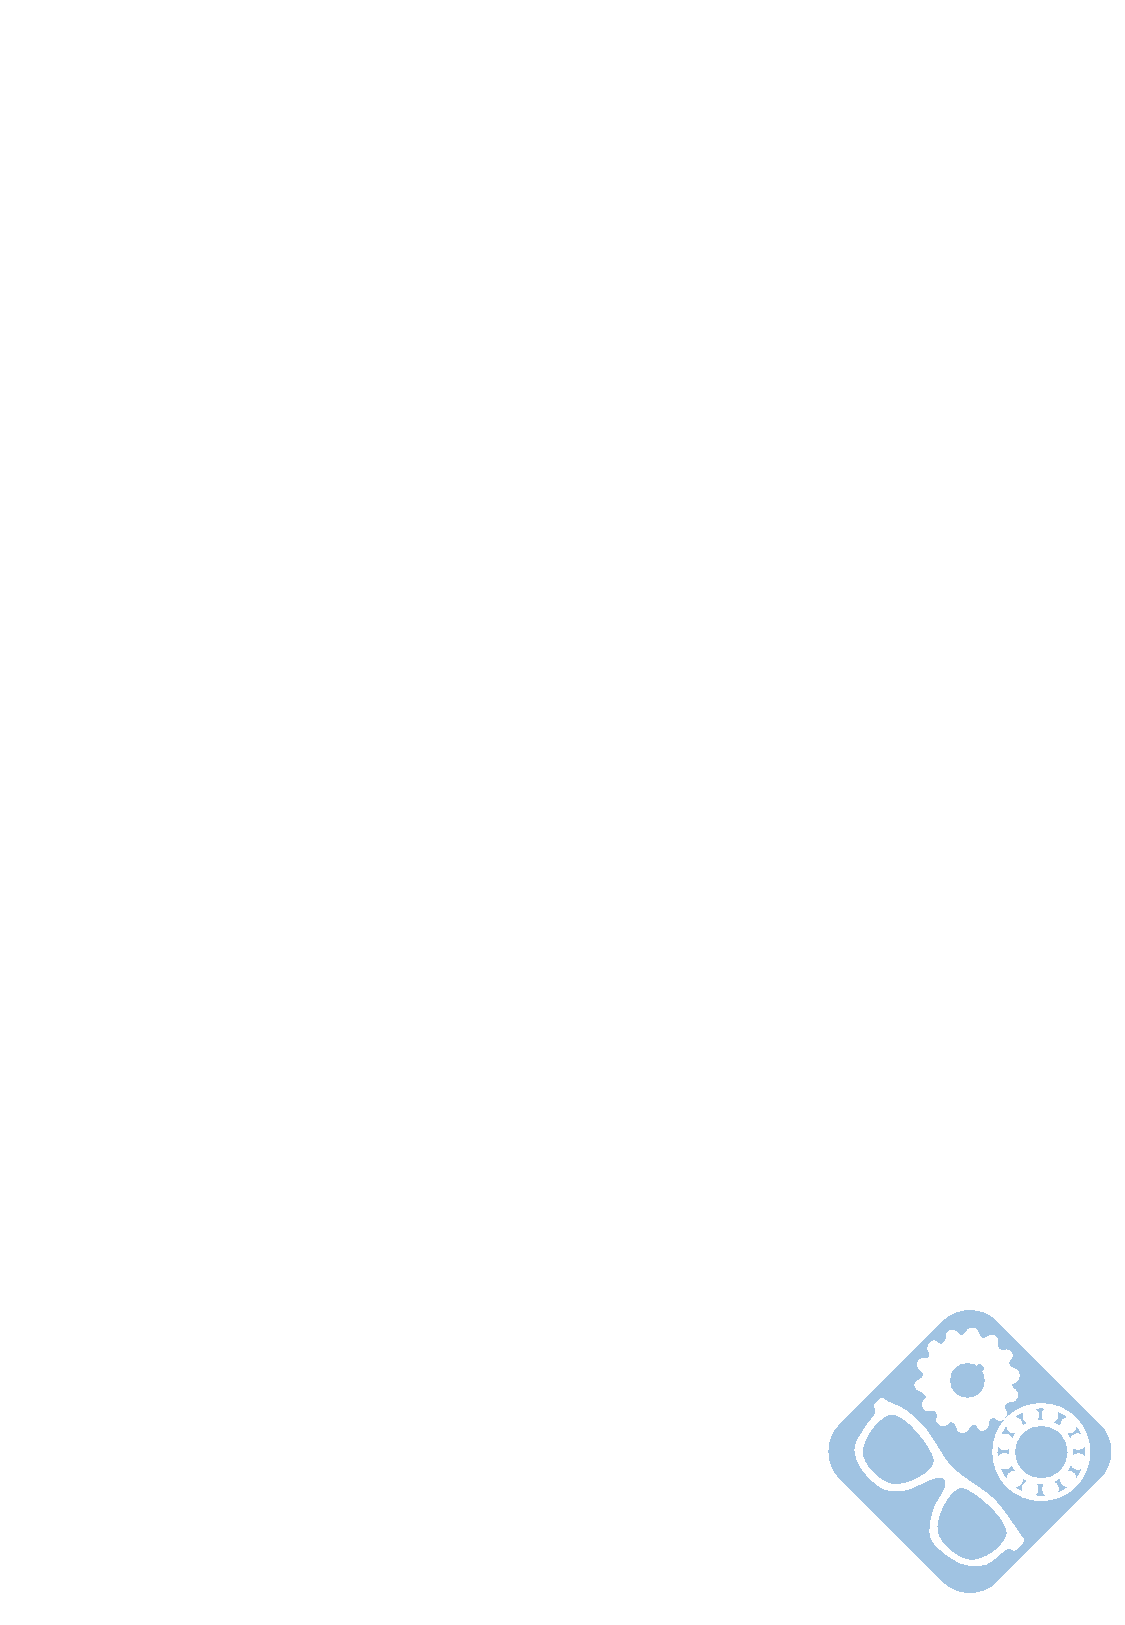
\includegraphics[width=\paperwidth,height=\paperheight,%
keepaspectratio]{../../../img/fond4}%
\end{center}
\vfill
}}}

\begin{document}

\pagestyle{empty}

\AddToShipoutPicture*{\BackgroundPic}


\includegraphics[width=2cm]{../../../img/logo}

\Huge{DS \numero - \sujet}

\vspace{1cm}

\ifdef{\prive}{\begin{center}\colorbox{danger}{\Huge{Avec Correction}}\end{center}}{}

\begin{center}
\centering\huge{PTSI}
\end{center}

\vspace{2cm}


\begin{center}
\centering\Large{\jour}
\end{center}

\vspace{2cm}

\normalsize

\tableofcontents

\newpage

\AddToShipoutPicture{\BackgroundPicdeux}

\pagestyle{fancy}

\begin{center}
\Huge \sujet
\end{center}


\normalsize


\section{Découverte du système (20 min)}

\subsection{Mise en situation}

Les treillis soudés sont utilisés en maçonnerie pour la réalisation d'ouvrages en béton armé.

~\

\begin{figure}[!h]
\centering
\begin{minipage}{0.35\linewidth}
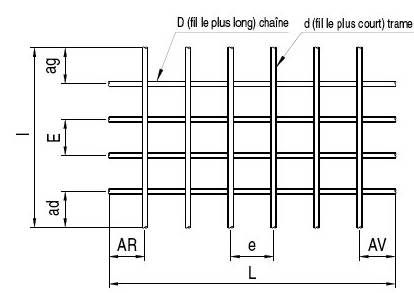
\includegraphics[width=\linewidth]{img/fig1}
\caption{Treillis}
\label{fig1}
\end{minipage}\hfill
\begin{minipage}{0.6\linewidth}
\begin{itemize}
 \item Largeur (l): 1200 mm,
 \item Longueur	(L): 6000 mm,
 \item Diamètre du fil longitudinal (chaine) (D): 7 mm,
 \item Diamètre du fil transversal (trame) (d): 7 mm,
 \item Pas transversal (E): 150 mm,
 \item Pas longitudinal	(e): 300 mm,
 \item Déports longitudinaux (AR), (AV): 150 mm,
 \item Déports transversaux	(ag), (ad): 75 mm.
\end{itemize}
\end{minipage}
\end{figure}

~\

Ces treillis sont fabriqués, à l'aide d'une soudeuse automatique, à partir de sections de « fils » métalliques : chaines et trames (voir figure \ref{fig1}). Après positionnement, une trame (diamètre d) est soudée simultanément en chaque point de contact avec les chaines (diamètre D). L'opération se répète sur la longueur, à chaque avance des chaines du pas e. En sortie de soudeuse, les extrémités des trames, composant le treillis, coulissent le long de 2 cornières.

\begin{figure}[!h]
\centering
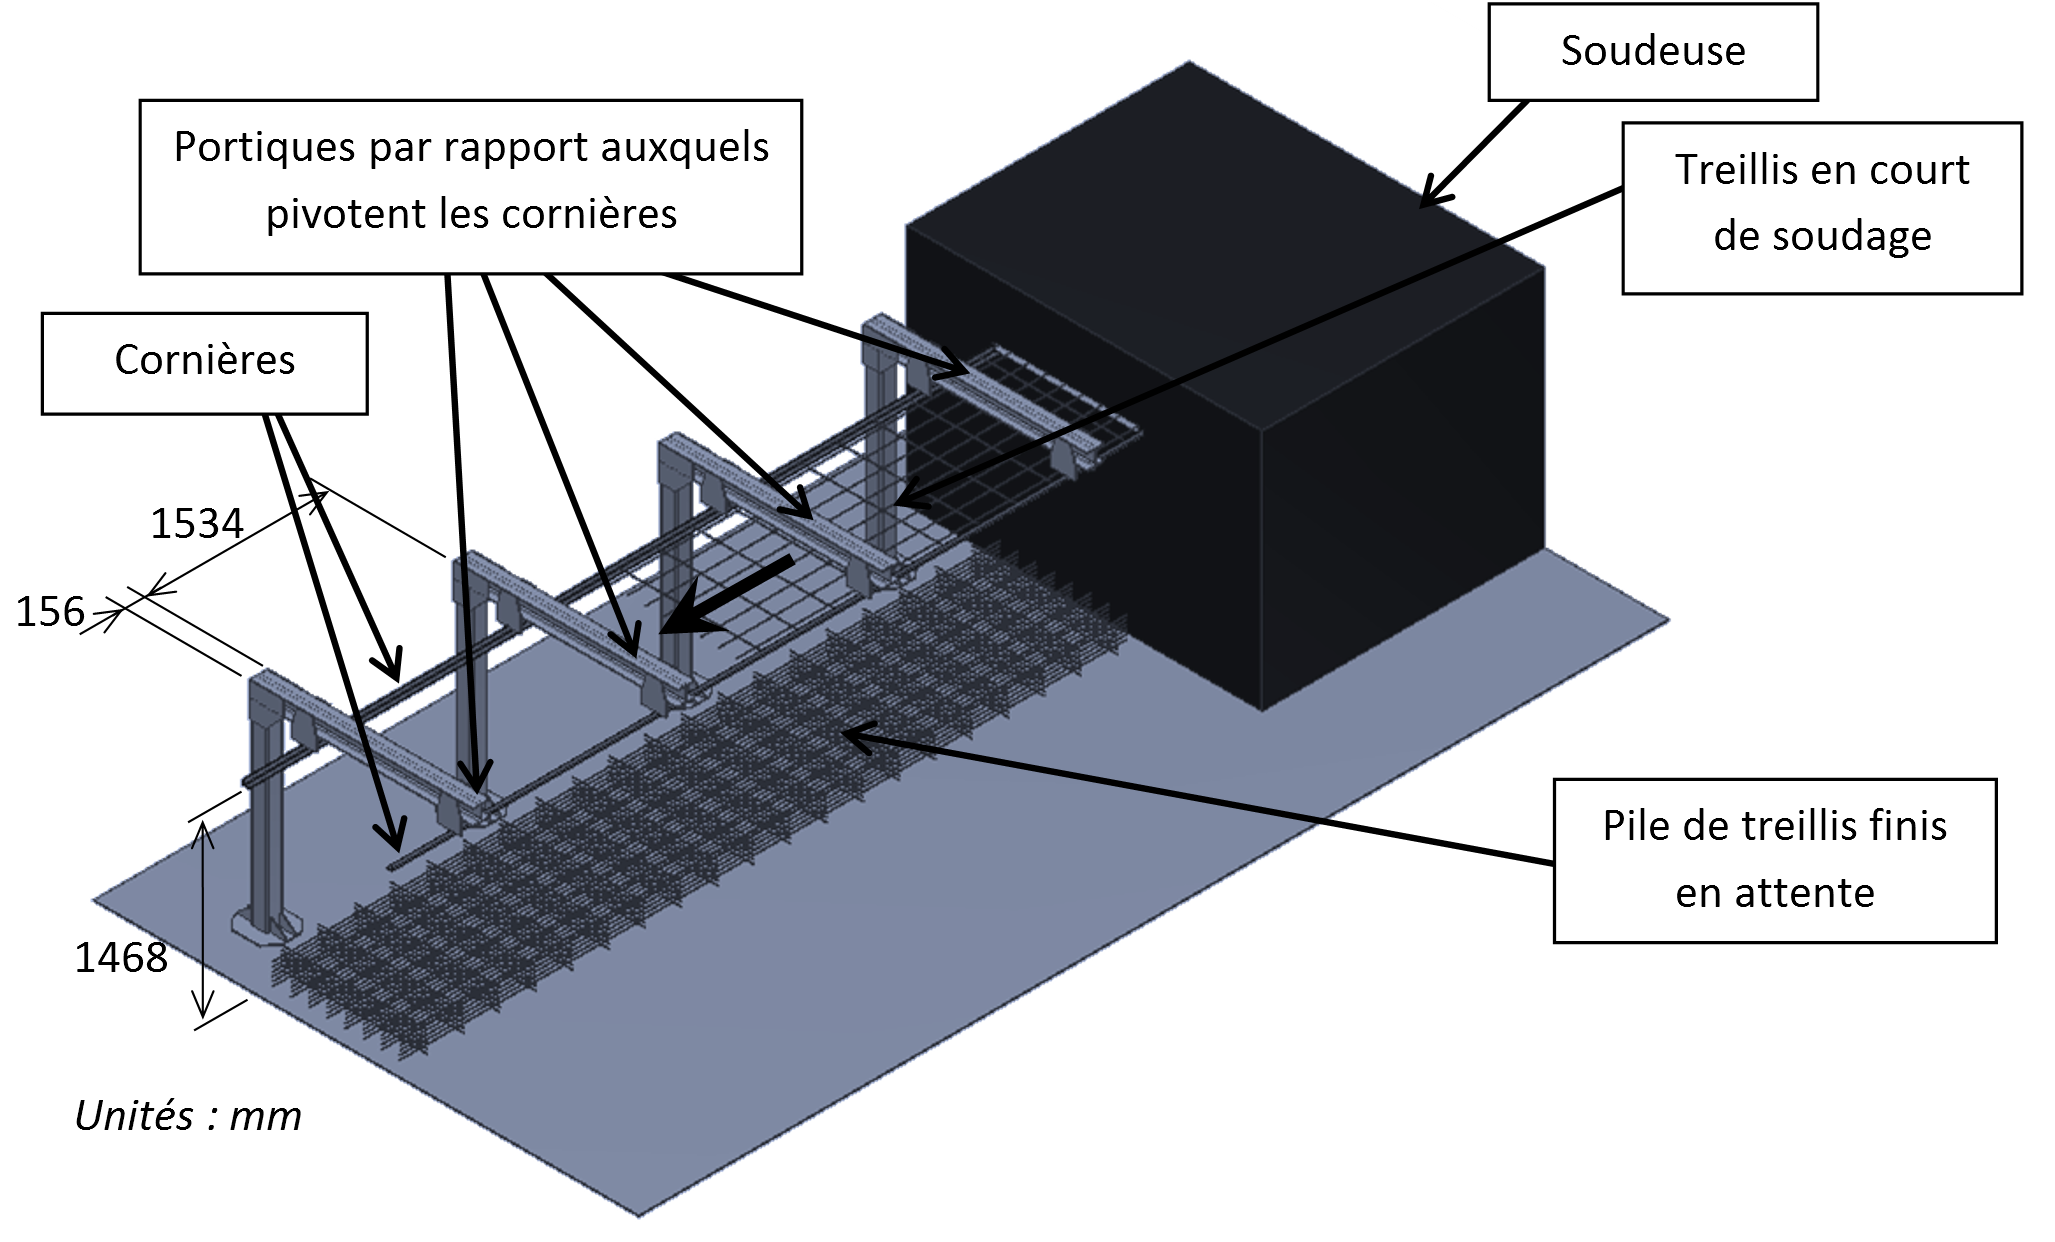
\includegraphics[width=0.6\linewidth]{img/fig2}
\caption{Poste de soudage}
\label{fig2}
\end{figure}

Une fois finis et après le pivotement des deux cornières (les cornières sont actionnées à l'aide d'un moto-réducteur par l'intermédiaire d'un mécanisme de renvoi qui n'est pas défini ici), les treillis tombent les uns sur les autres d'une hauteur  maximale de 1,4 m. Lorsque 60 treillis sont empilés, la soudeuse s'arrête, un opérateur cercle la pile de treillis et l'évacue à l'aide d'un chariot élévateur. Les opérations de cerclage et d'évacuation stoppent la production de treillis pendant 15 minutes.

\textbf{Un système automatique permettant la manutention des treillis en sortie de soudeuse a été préconçu pour limiter les nuisances sonores dues à la chute des treillis et pour optimiser la production.}

\subsection{Diagramme de contexte (incomplet)}

\begin{figure}[!h]
\centering
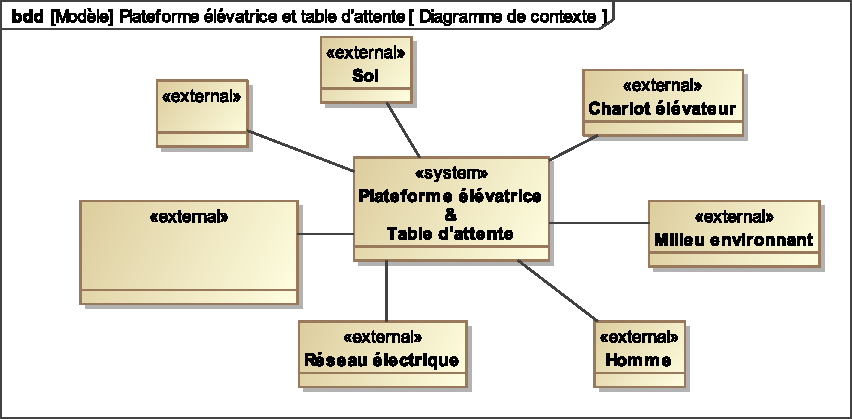
\includegraphics[width=0.7\linewidth]{img/Diagramme_de_contexte_vide}
\caption{Diagramme de contexte (incomplet)}
\label{Diagramme_de_contexte_vide}
\end{figure}


\subsection{Diagramme d'exigences}

\begin{figure}[!h]
\centering
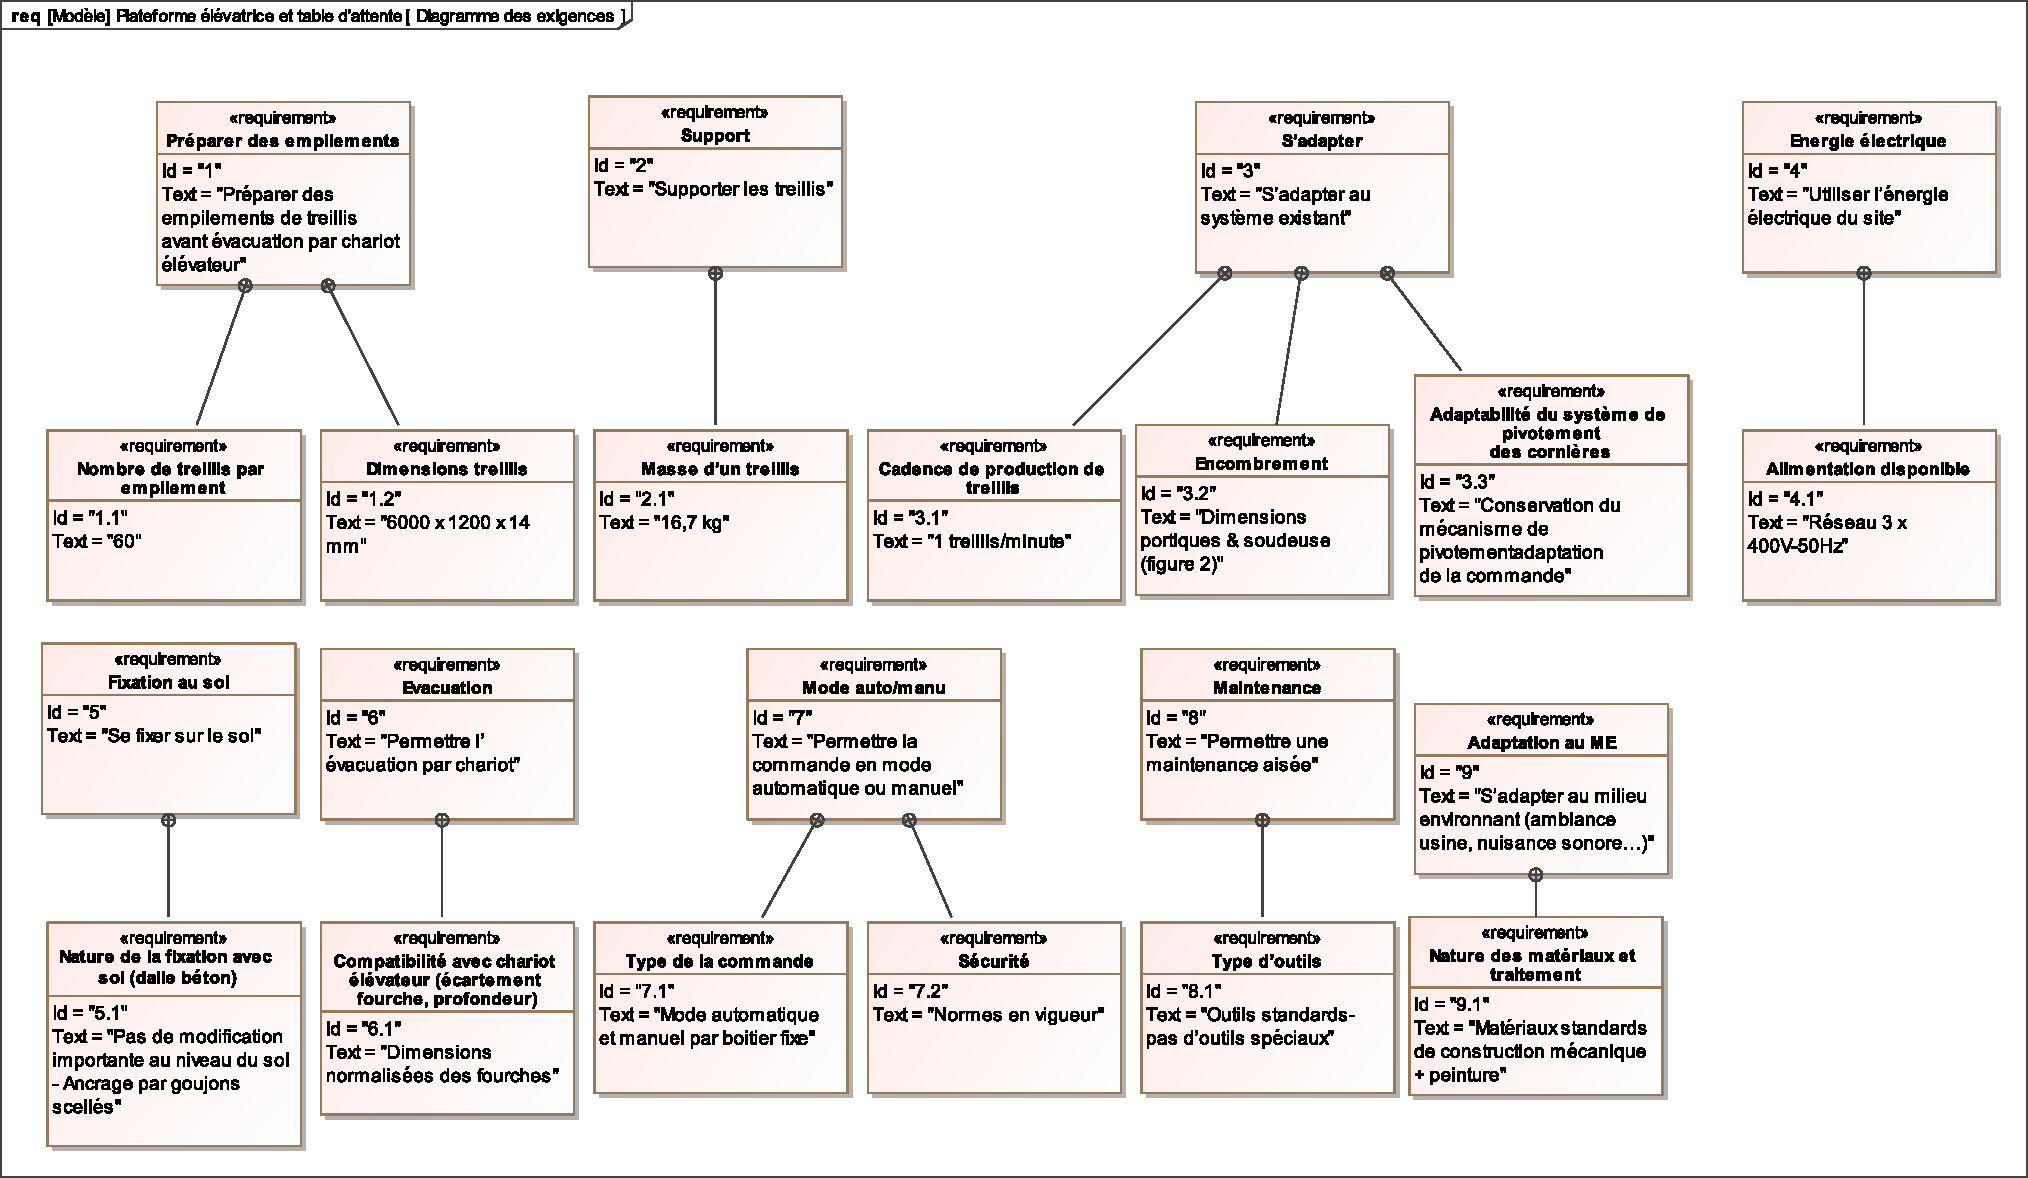
\includegraphics[width=\linewidth]{img/Diagramme_des_exigences}
\caption{Diagramme des exigences}
\label{Diagramme_des_exigences}
\end{figure}

\subsection{Présentation du système préconçu}

Le concepteur s'est orienté vers un système composé d'une table élévatrice et d'une table d'attente, et a conservé les portiques et les cornières.

La table élévatrice va permettre de réceptionner les treillis finis en limitant leur chute et d'évacuer la pile de 60 treillis sur la table d'attente. L'opérateur pourra ensuite cercler la pile de treillis sans arrêter la production de treillis.

La table élévatrice permet le déplacement suivant 2 axes :
\begin{itemize}
 \item un axe vertical motorisé par l'association d'un moteur à courant continu et de 3 vérins à vis ;
 \item un axe horizontal composé de 2 pousseurs entraînés par 2 dispositifs pignons chaine et motorisé par un moto-réducteur asynchrone.
\end{itemize}

\begin{figure}[!h]
\centering
\begin{minipage}{0.45\linewidth}
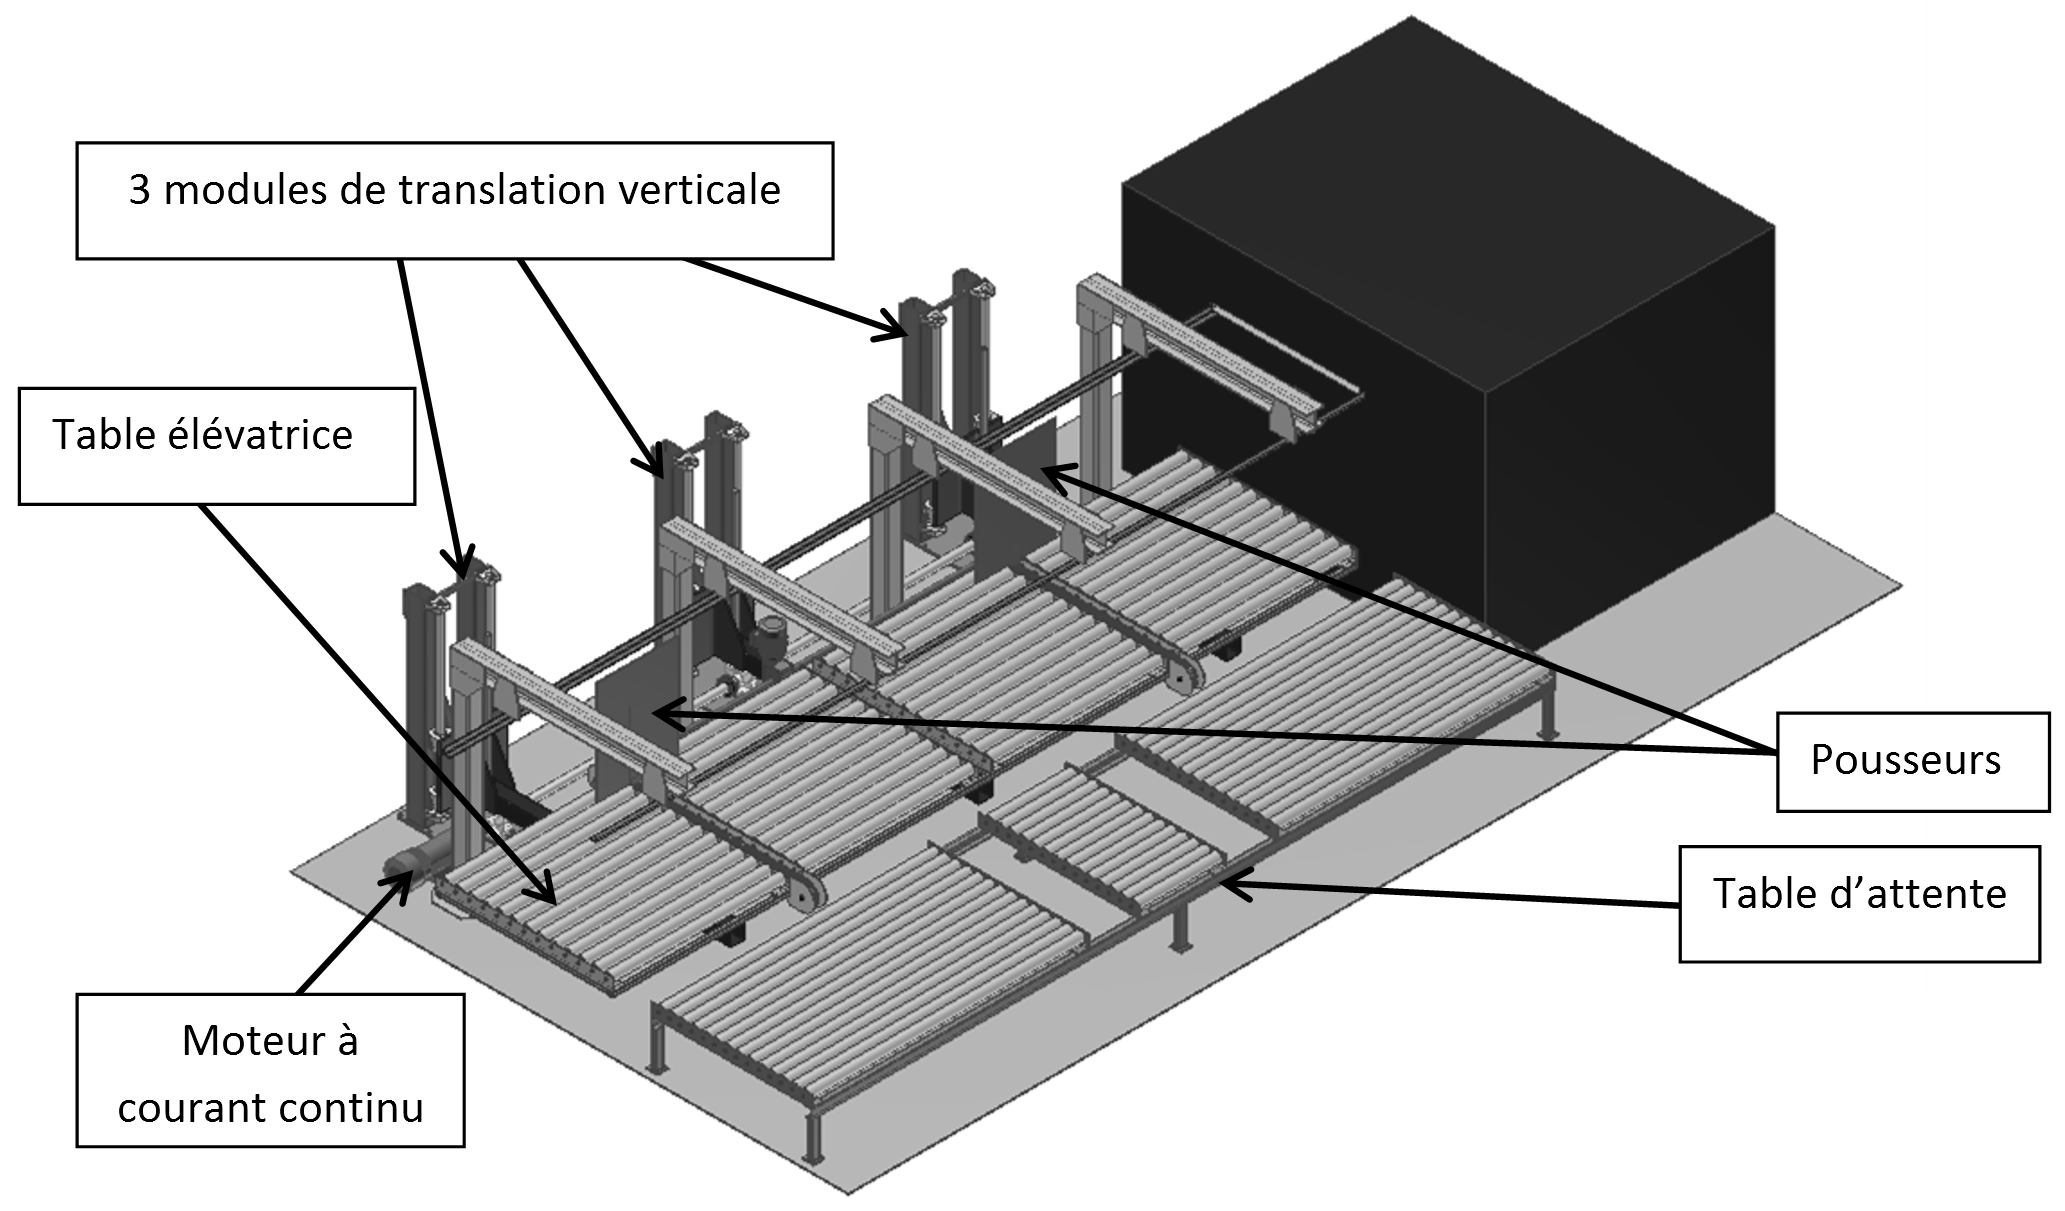
\includegraphics[width=\linewidth]{img/fig3}
\caption{Poste de soudage}
\label{fig3}
\end{minipage}\hfill
\begin{minipage}{0.45\linewidth}
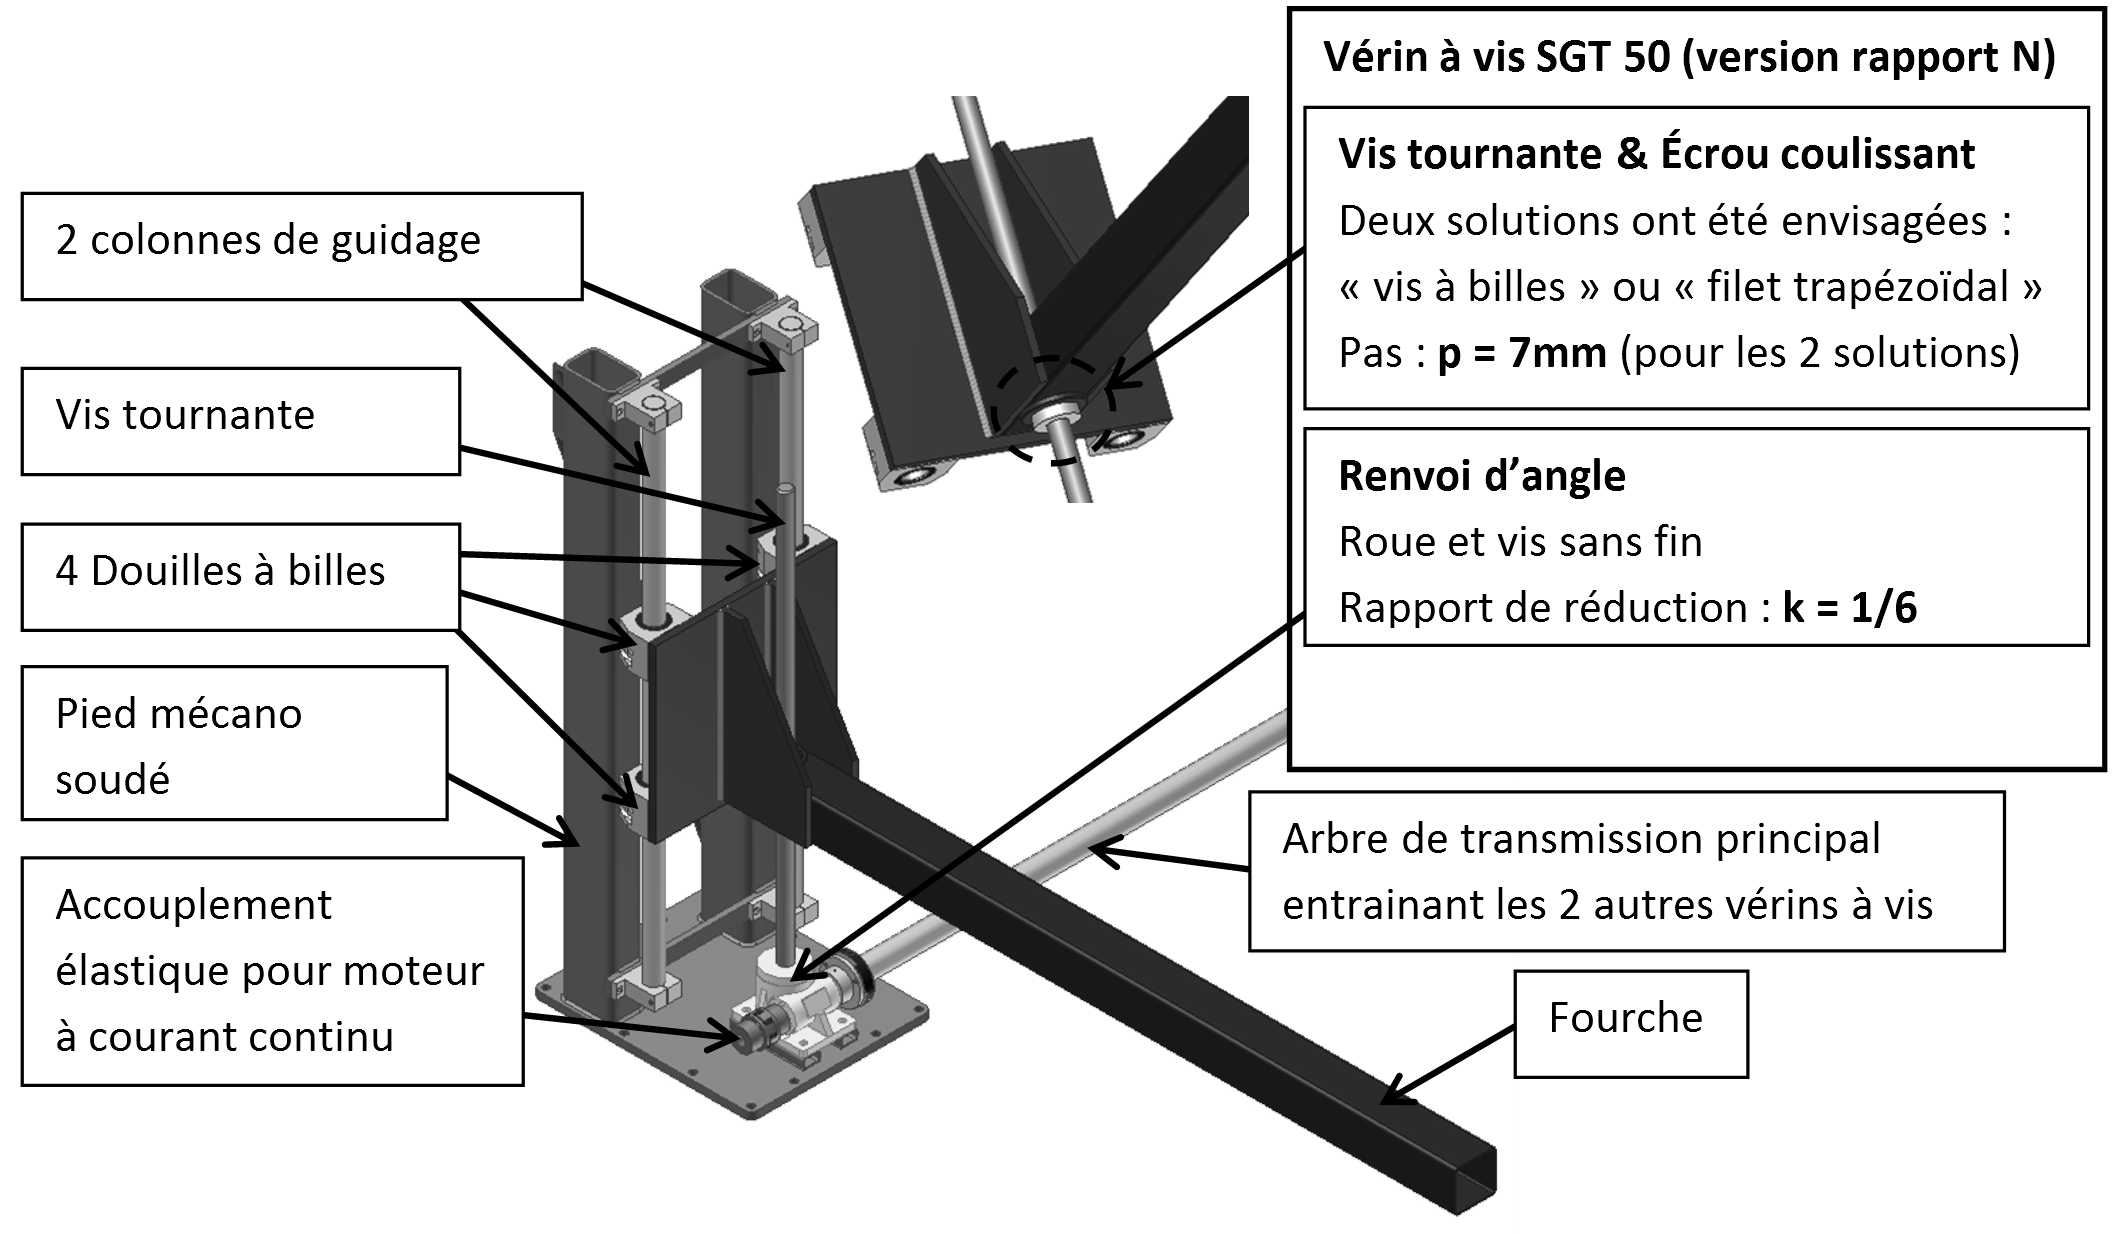
\includegraphics[width=\linewidth]{img/fig4}
\caption{Module de translation verticale}
\label{fig4}
\end{minipage}
\end{figure}

\begin{figure}[!h]
\centering
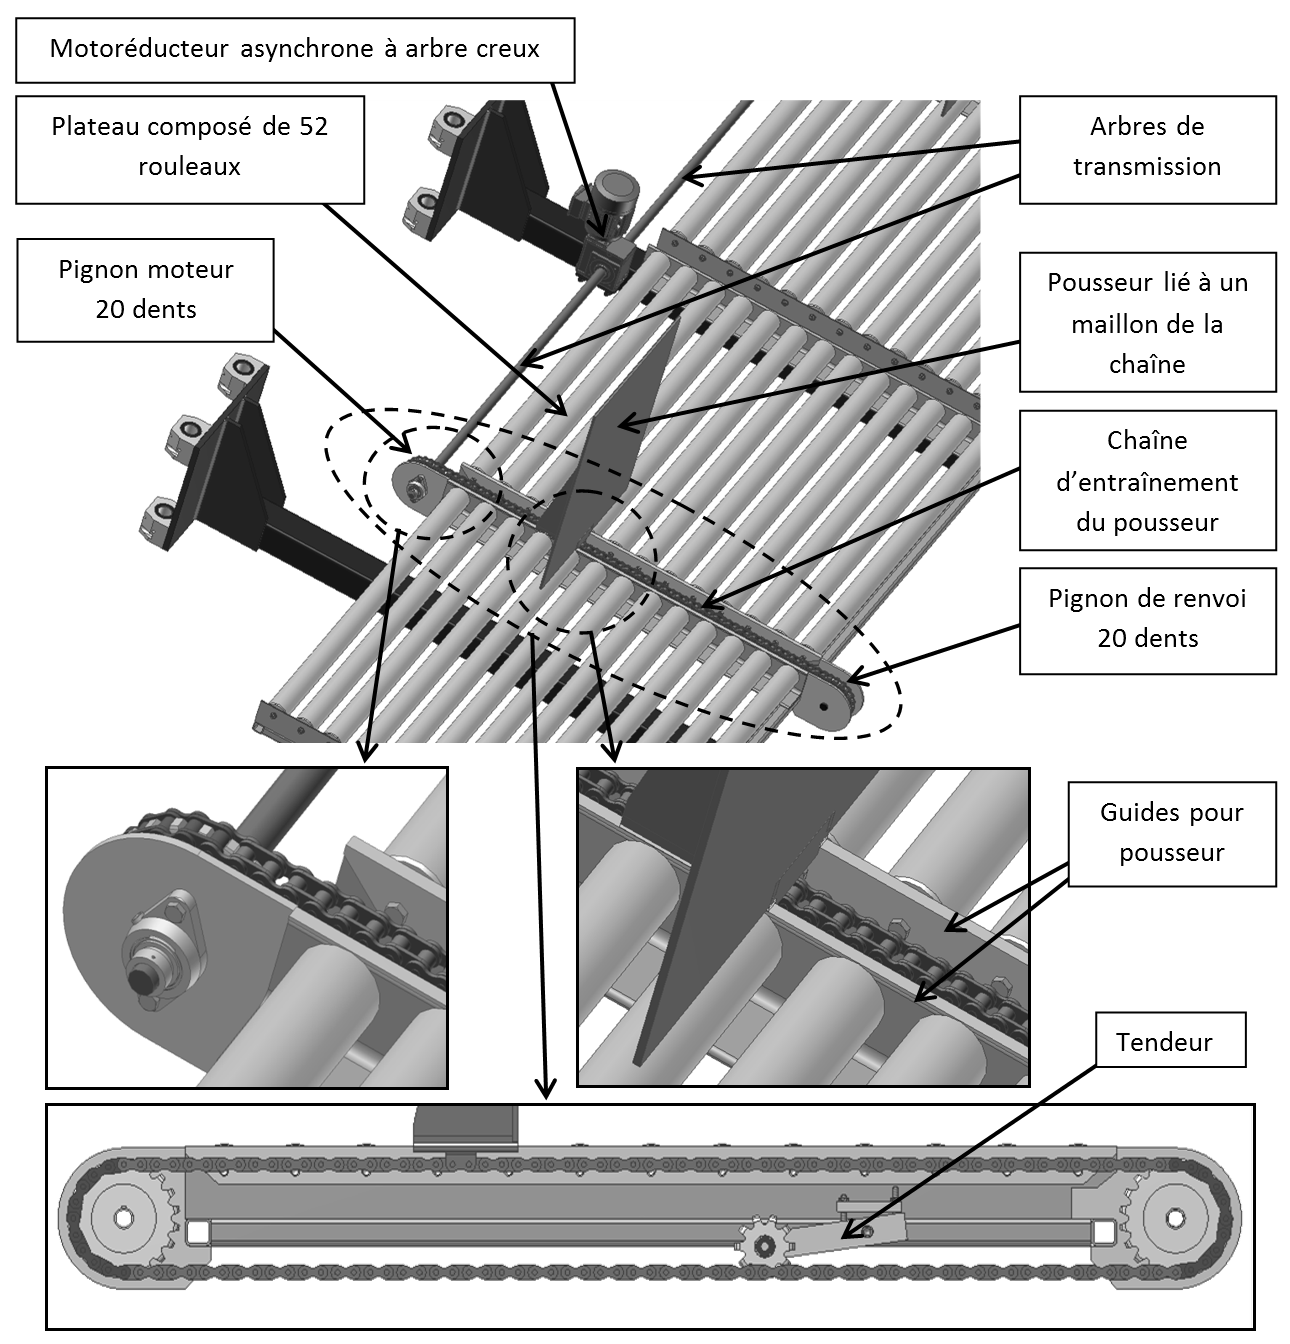
\includegraphics[width=0.6\linewidth]{img/fig5}
\caption{Pousseurs}
\label{fig5}
\end{figure}

\subsection{Problématique}

\textbf{L'objectif général de l'étude consiste à valider certaines solutions constructives et à définir des éléments de commande.}

Le concepteur a opté pour une solution électromécanique qui doit s'intégrer au système existant. Des choix ont été faits en termes d'architecture de mécanisme qu'il convient de vérifier.

Le moteur à courant continu, qui agit sur le déplacement vertical de la table élévatrice, sera sollicité avec des régimes très variés (montée à vide, descente en charge variable, montée en charge,...). Il faut vérifier la capacité du moteur pré-sélectionné et définir sa commande.

\section{Analyse du système (20 min)}

\paragraph{Question 1:} Compléter le diagramme de contexte du document réponse.

~\

Le système fonctionne 11h/24h, 5 jours/7, 44 semaines par an. Il est parfois arrêté à cause de pannes mais on considère qu'il n'est arrêté que 5\% du temps de fonctionnement.

\paragraph{Question 2:} Déterminer combien de treillis sont fabriqués par an.

\section{Étude de l'exigence \og Guider et Entrainer les treillis \fg (1h20min)}

\subsection{Étude de l'exigence \og Guider les treillis \fg}

L'objectif de cette partie est de valider l'architecture proposée au niveau du guidage en translation de la table élévatrice par rapport au bâti et de spécifier les contraintes liées à cette solution.

\paragraph{Question 3:} Évaluer le degré d'hyperstatisme du mécanisme dans la boucle A d'après le schéma cinématique minimal de la figure \ref{fig8}.

\paragraph{Question 4:}	Quelle(s) préconisation(s) peuvent être proposée(s) au montage pour contourner cet hyperstatisme.

\paragraph{Question 5:} La liaison glissière est réalisée par 4 douilles à billes et 2 colonnes de guidage. Évaluer le degré d'hyperstatisme propre à la réalisation de cette liaison glissière d'après le schéma architectural de la figure \ref{fig10}.

On souhaite vérifier le bon dimensionnement du vérin à vis SGT50 pour cette application. Lorsque l'écrou est en position haute, il a parcouru un peu moins de 0,9 m. Le poids de la fourche sera négligé.

\paragraph{Question 6:} D'après le tableau de la figure \ref{fig6}, justifier que le pas de la vis est bien égal à $7mm$.

L'objectif de cette partie est de vérifier la capacité de charge des douilles à billes. Les douilles seront le plus sollicitées quand le chargement sera maximal (pile de treillis complète). Les accélérations de la table étant faibles lors des déplacements, on pourra, dans ce cas, négliger les composantes dynamiques et se ramener à un problème statique. Le raisonnement portera \textbf{sur un module de translation verticale}.

Le problème étant hyperstatique, il sera traité en 2 temps :
\begin{itemize}
 \item dans un premier temps, à l'aide du schéma cinématique minimal figure \ref{fig8}, déterminer complètement l'action mécanique exercée par le bâti (0) sur la fourche(1),
 \item dans un second temps, à l'aide des documents constructeurs figure \ref{fig11}, déterminer les charges radiales supportées par chaque douille à billes.
\end{itemize}

Hypothèses et données :
\begin{itemize}
 \item la liaison glissière est supposée parfaite,
 \item on suppose que chaque fourche d'un module de translation verticale reprend la même charge, l'action mécanique exercée par la pesanteur sur la fourche (1) avec son chargement est donc représentée par un glisseur d'axe $(C,\overrightarrow{Y})$ de module 5000 N (figure \ref{fig8}),
 \item l'action mécanique exercée par la vis (2) sur la fourche (1) est supposée pouvoir s'exprimer, d'après les dispositions constructives, par le torseur suivant :
$\left\{T_{2\rightarrow 1}\right\}=\left\{\begin{array}{cc}0 & 0 \\ Y_{B 2\rightarrow 1} & M_{B 2\rightarrow 1} \\ 0 & 0\end{array}\right\}_{B,(\overrightarrow{X},\overrightarrow{Y},\overrightarrow{Z})}$
Les documents constructeurs permettent de connaître les caractéristiques suivantes :
\begin{itemize}
 \item $M_{B 2\rightarrow 1}=0,0035.Y_{B 2\rightarrow 1}$, pour une \og vis trapézoïdale \fg,
 \item $M_{B 2\rightarrow 1}=0,0012.Y_{B 2\rightarrow 1}$, pour une \og vis à billes \fg, avec $M_{2\rightarrow1}$ en N.m et $Y_{2\rightarrow1}$ en N.
\end{itemize}
 \item capacité de charge statique d'une douille : $C_0=8,28kN$.
\end{itemize}

\paragraph{Question 7:} Effectuer le bilan des actions mécaniques extérieures exercées sur la fourche (1) avec son chargement. Les actions seront représentées par des torseurs sous la forme suivante :

$\left\{T_{i\rightarrow j}\right\}=\left\{\begin{array}{cc} X_{O i\rightarrow j} & L_{O i\rightarrow j} \\ Y_{O i\rightarrow j} & M_{O i\rightarrow j} \\ Z_{O i\rightarrow j} & N_{O i\rightarrow j} \end{array}\right\}_{O,(\overrightarrow{X},\overrightarrow{Y},\overrightarrow{Z})}$

\paragraph{Question 8:} Appliquer le principe fondamental de la statique à la fourche (1) avec son chargement, et en déduire les équations scalaires utiles à la résolution.

\paragraph{Question 9:} Déterminer les composantes du torseur représentant l'action mécanique exercée par le bâti (0) sur la fourche (1) dans les 2 configurations : « vis à billes » et « vis trapézoïdale ».

\paragraph{Question 10:} En exploitant la figure \ref{fig11}, déterminer les charges normales et transversales supportées par chaque douille dans le cas le plus défavorable et vérifier la capacité de charge des douilles en statique.

\section{Étude de l'exigence: \og Entrainer les treillis \fg (1h)}

L'objectif de cette partie est d'étudier le dimensionnement du moteur d'entrainement du treillis en terme de couple.

Attention, dans cette partie, le raisonnement portera sur l'ensemble de la table élévatrice.

Hypothèses et données :
\begin{itemize}
 \item les liaisons des différents éléments avec le bâti (0) sont supposées parfaites,
 \item la masse M de l'ensemble mobile verticalement noté \{A\}=\{fourches, plateau avec son chargement,...\} varie de 500 kg (sans treillis)  à 1500 kg (avec les 60 treillis),
 \item on prendra $g=10m/s^2$ pour l'accélération de la pesanteur,
 \item on donne le torseur des actions mécaniques exercées par la pesanteur sur l'ensemble mobile \{A\}: \\
$\left\{T_{pes\rightarrow \{A\}}\right\}=\left\{\begin{array}{cc} 0 & 0 \\ -M.g & 0 \\ 0 & 0 \end{array}\right\}_{G,(\overrightarrow{X},\overrightarrow{Y},\overrightarrow{Z})}$, G est le centre de gravité de l'ensemble mobile \{A\},
 \item on donne le torseur cinématique de l'ensemble mobile \{A\} dans son mouvement :
 $\left\{V_{\{A\}/R_0}\right\}=\left\{\begin{array}{cc} 0 & 0 \\ 0 & V \\ 0 & 0 \end{array}\right\}_{P,(\overrightarrow{X},\overrightarrow{Y},\overrightarrow{Z})}$, P est un point quelconque de l'ensemble mobile \{A\},
 \item caractéristiques des vérins à vis :
 \begin{itemize}
  \item Pas (p): $7mm$,
  \item Rapport de réduction (k): $\frac{1}{6}$,
  \item Rendement $\eta_v=0,5$ (dispositif avec vis à billes).
   \end{itemize}
 \item le moteur fournit un couple $Cm_m$ pour la montée et un couple $Cm_d$ pour la descente,
 \item l'étude s'effectuera dans le pire des cas,
 \item la vitesse angulaire du moteur sera notée $\omega_m$ et l'accélération angulaire sera notée $\dot{\omega}_m$,
 \item l'inertie équivalente ramenée sur l'arbre moteur est $J_{eq}=5.42*10^{-2}kg.m^2$.
\end{itemize}

On donne le théorème du moment du principe fondamental de la dynamique appliqué sur l'arbre moteur: $J_{eq}.\frac{d\omega_m(t)}{dt}=C_m(t)-C_P(t)$, avec $C_P(t)$ couple lié au poids ramené à l'arbre moteur, déterminé par l'équation $C_P(t)=\frac{\eta.M.g.p.k}{2.\pi}$.

Le profil de vitesse souhaité est présenté à la figure \ref{profil}, il permet en théorie un déplacement de 0,9m.

\begin{figure}[!h]
\centering
 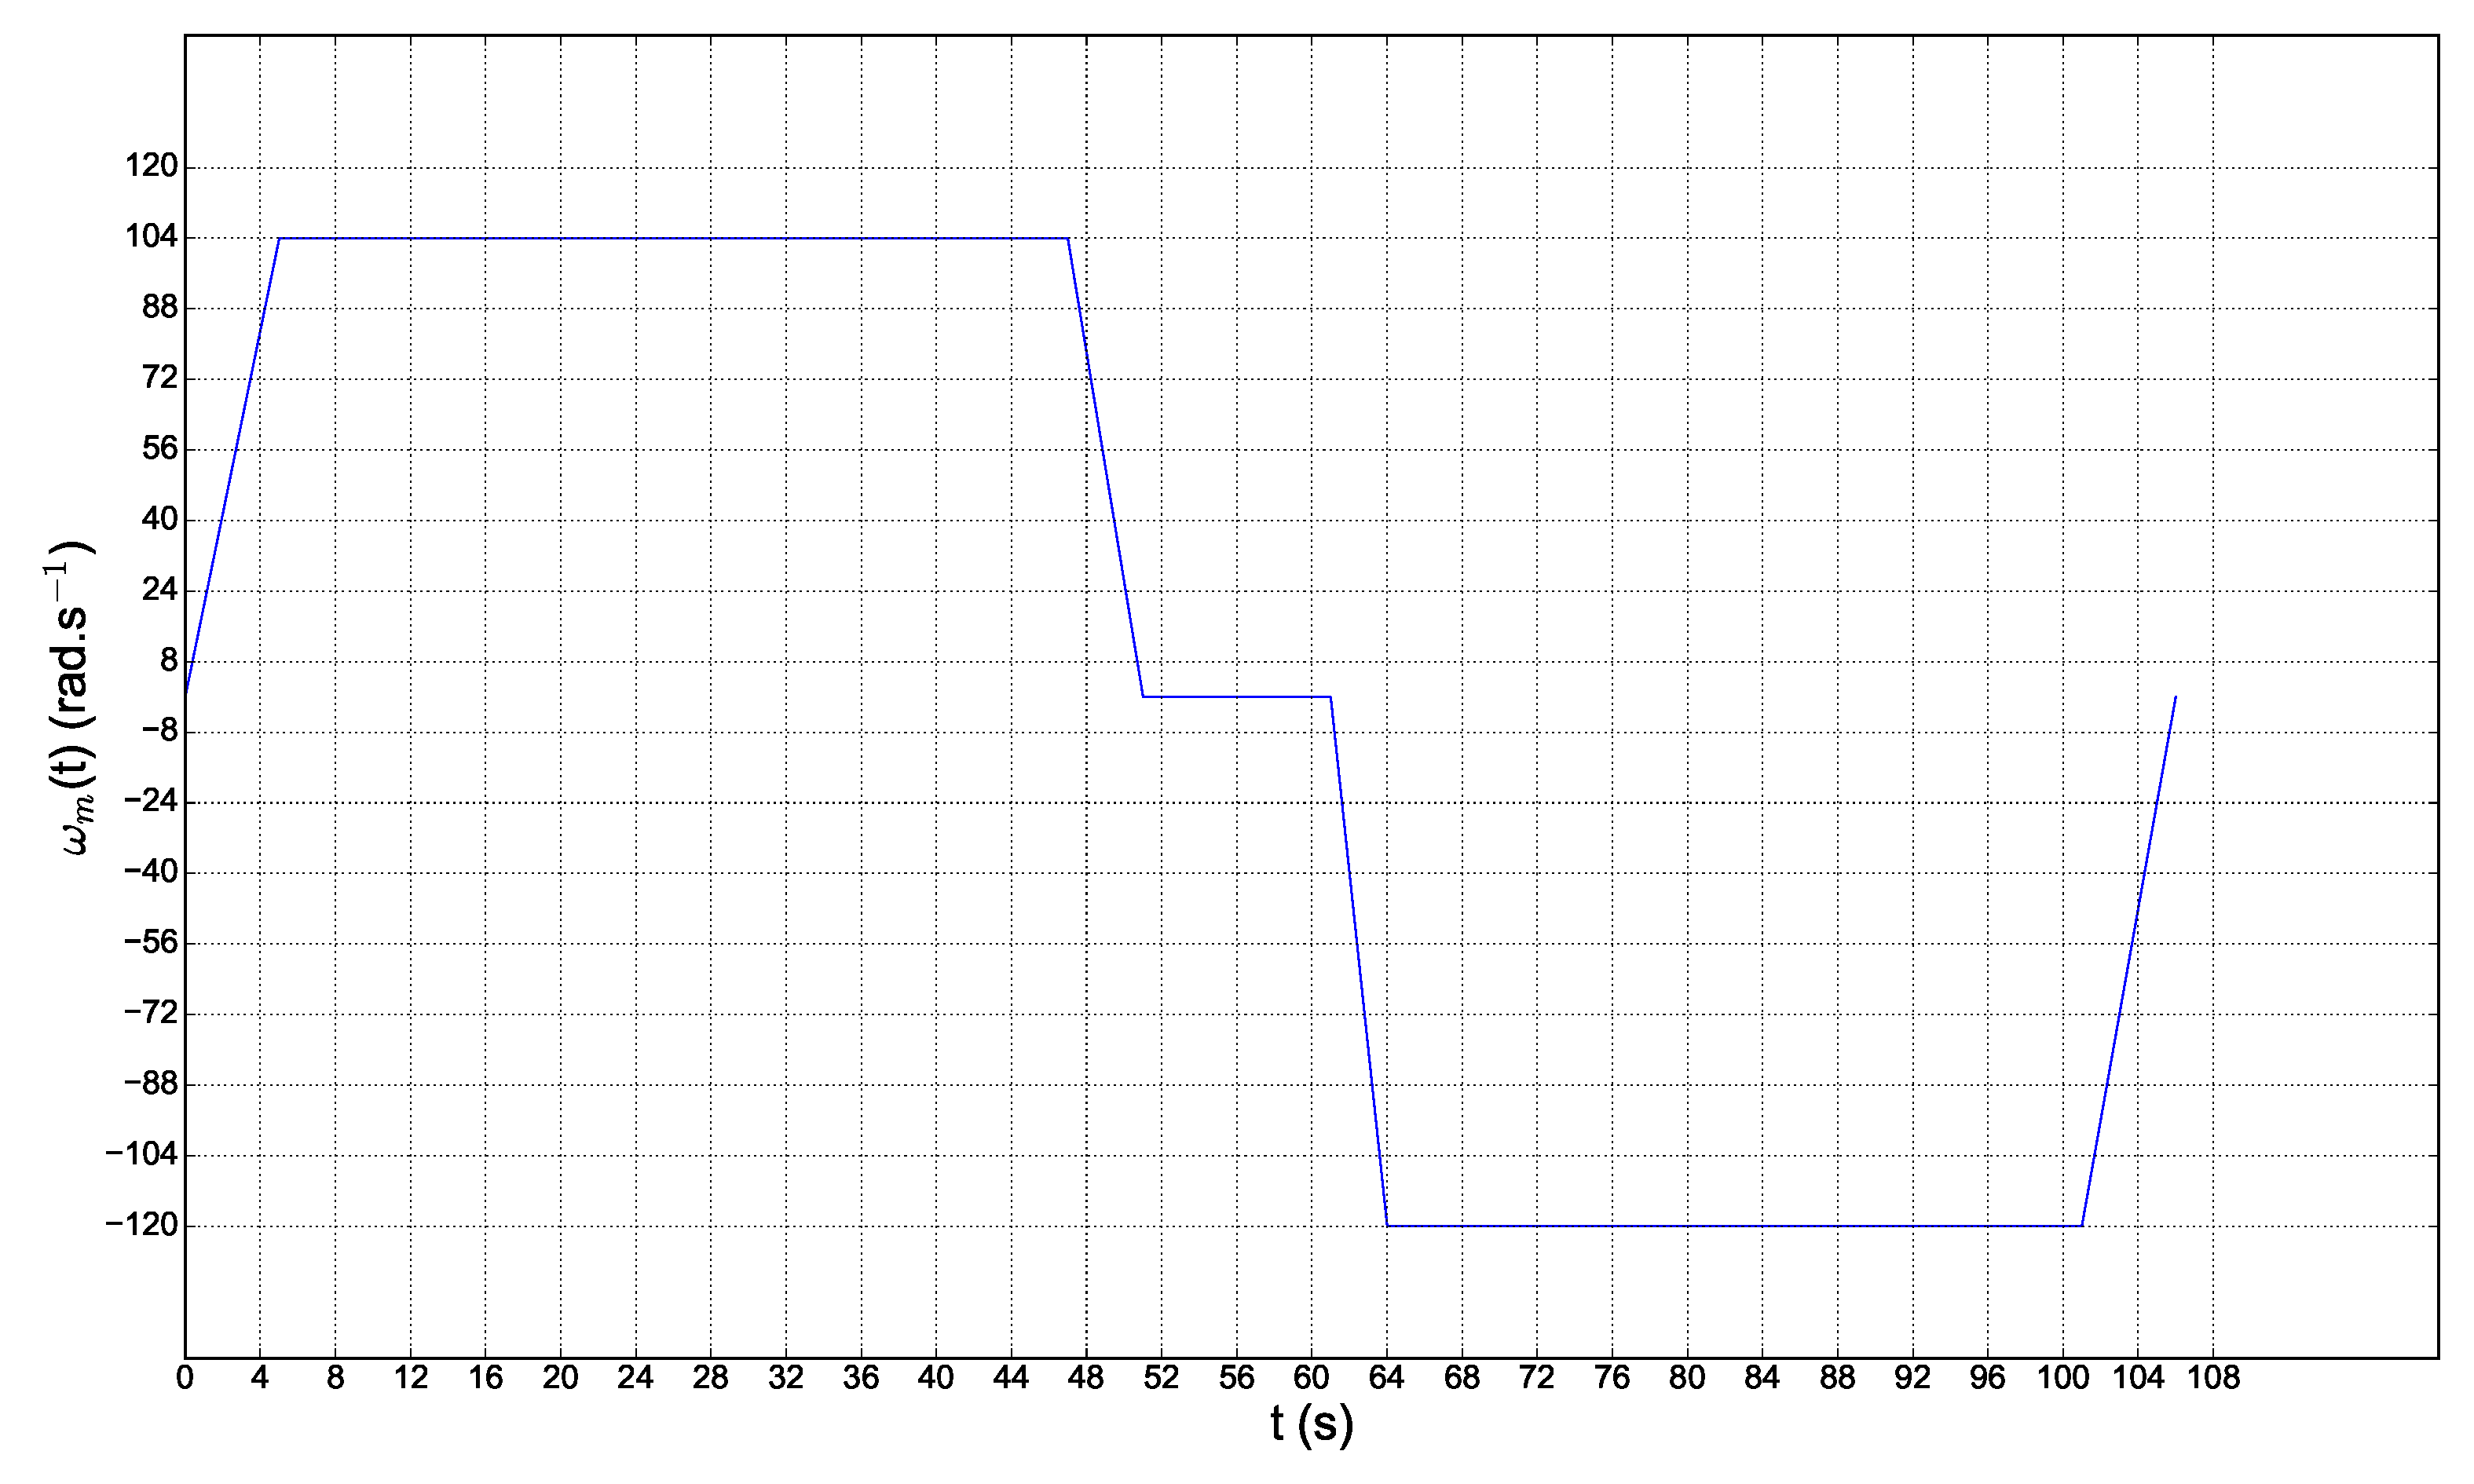
\includegraphics[width=0.9\linewidth]{img/profil}
\caption{Profil de vitesse}
\label{profil}
\end{figure}

\paragraph{Question 11:} Tracer sur le document réponse le profil d'accélération correspondant à celui de vitesse de la figure \ref{profil}.

\paragraph{Question 12:} En utilisant le théorème du moment du principe fondamental de la dynamique, tracer sur le document réponse l'allure du couple moteur $C_m(t)$. Justifier la réponse.

Les caractéristiques nominales du moteur à courant continu choisi sont répertoriées dans le tableau \ref{moteur}.

\begin{table}[!h]
\centering
\begin{tabular}{|c|c|c|c|c|c|c|}
\hline
P ($kW$) & N ($tr.min^{-1}$) & C ($N.m$) & U ($V$) & I ($A$) & R ($\Omega$) & Ke ($V.rad^{-1}.s$)\\
\hline
0,73 & 1080 & 6,46 & 230 & 4 & 5,22 & 1,6 \\
\hline
\end{tabular}
\caption{Caractéristiques du moteur électrique}
\label{moteur}
\end{table}

\paragraph{Question 13:} Justifier que le moteur choisi correspond aux performances attendues.

\paragraph{Question 14:} Tracer sur le document réponse le profil du déplacement de la table $d_t(t)$. La position initiale sera nulle $d_t(0)=0$.

\paragraph{Question 15:} Justifier que le déplacement correspond à celui du cahier des charges.

\section{Pilotage du moteur à courant continu (1h)}

L'objectif de cette partie est de déterminer le profil de tension à soumettre au moteur électrique afin de générer le mouvement souhaité.

\paragraph{Question 16:} Déterminer les équations électriques du moteur liant, $u_m(t)$, $i(t)$, $e(t)$, $C_m(t)$ et $\omega_m(t)$ en fonction de $R$, $L$, $K_e$ et $K_c$.

\paragraph{Question 17:} En déduire $u(t)$ en fonction de $C_m(t)$ et $\omega_m(t)$ et des caractéristiques électriques du moteur. 

Pour la suite, on va considérer la valeur de l'inductance $L$ comme négligeable.

\paragraph{Question 18:} Donner la nouvelle équation de $u(t)$.

\paragraph{Question 19:} Tracer $u(t)$ sur le document réponse.

\paragraph{Question 20:} Cette valeur est-elle compatible avec les caractéristiques nominales du moteur ?

\paragraph{Question 21:} Les questions 18 et 19 auraient-elles été possibles sans l'hypothèse de l'inductance nulle $L=0$ ?

\paragraph{Question 22:} Critiquer alors le modèle du profil donné sur la figure \ref{profil}.

\newpage

\section{Annexes}

~\

\begin{figure}[!h]
\centering
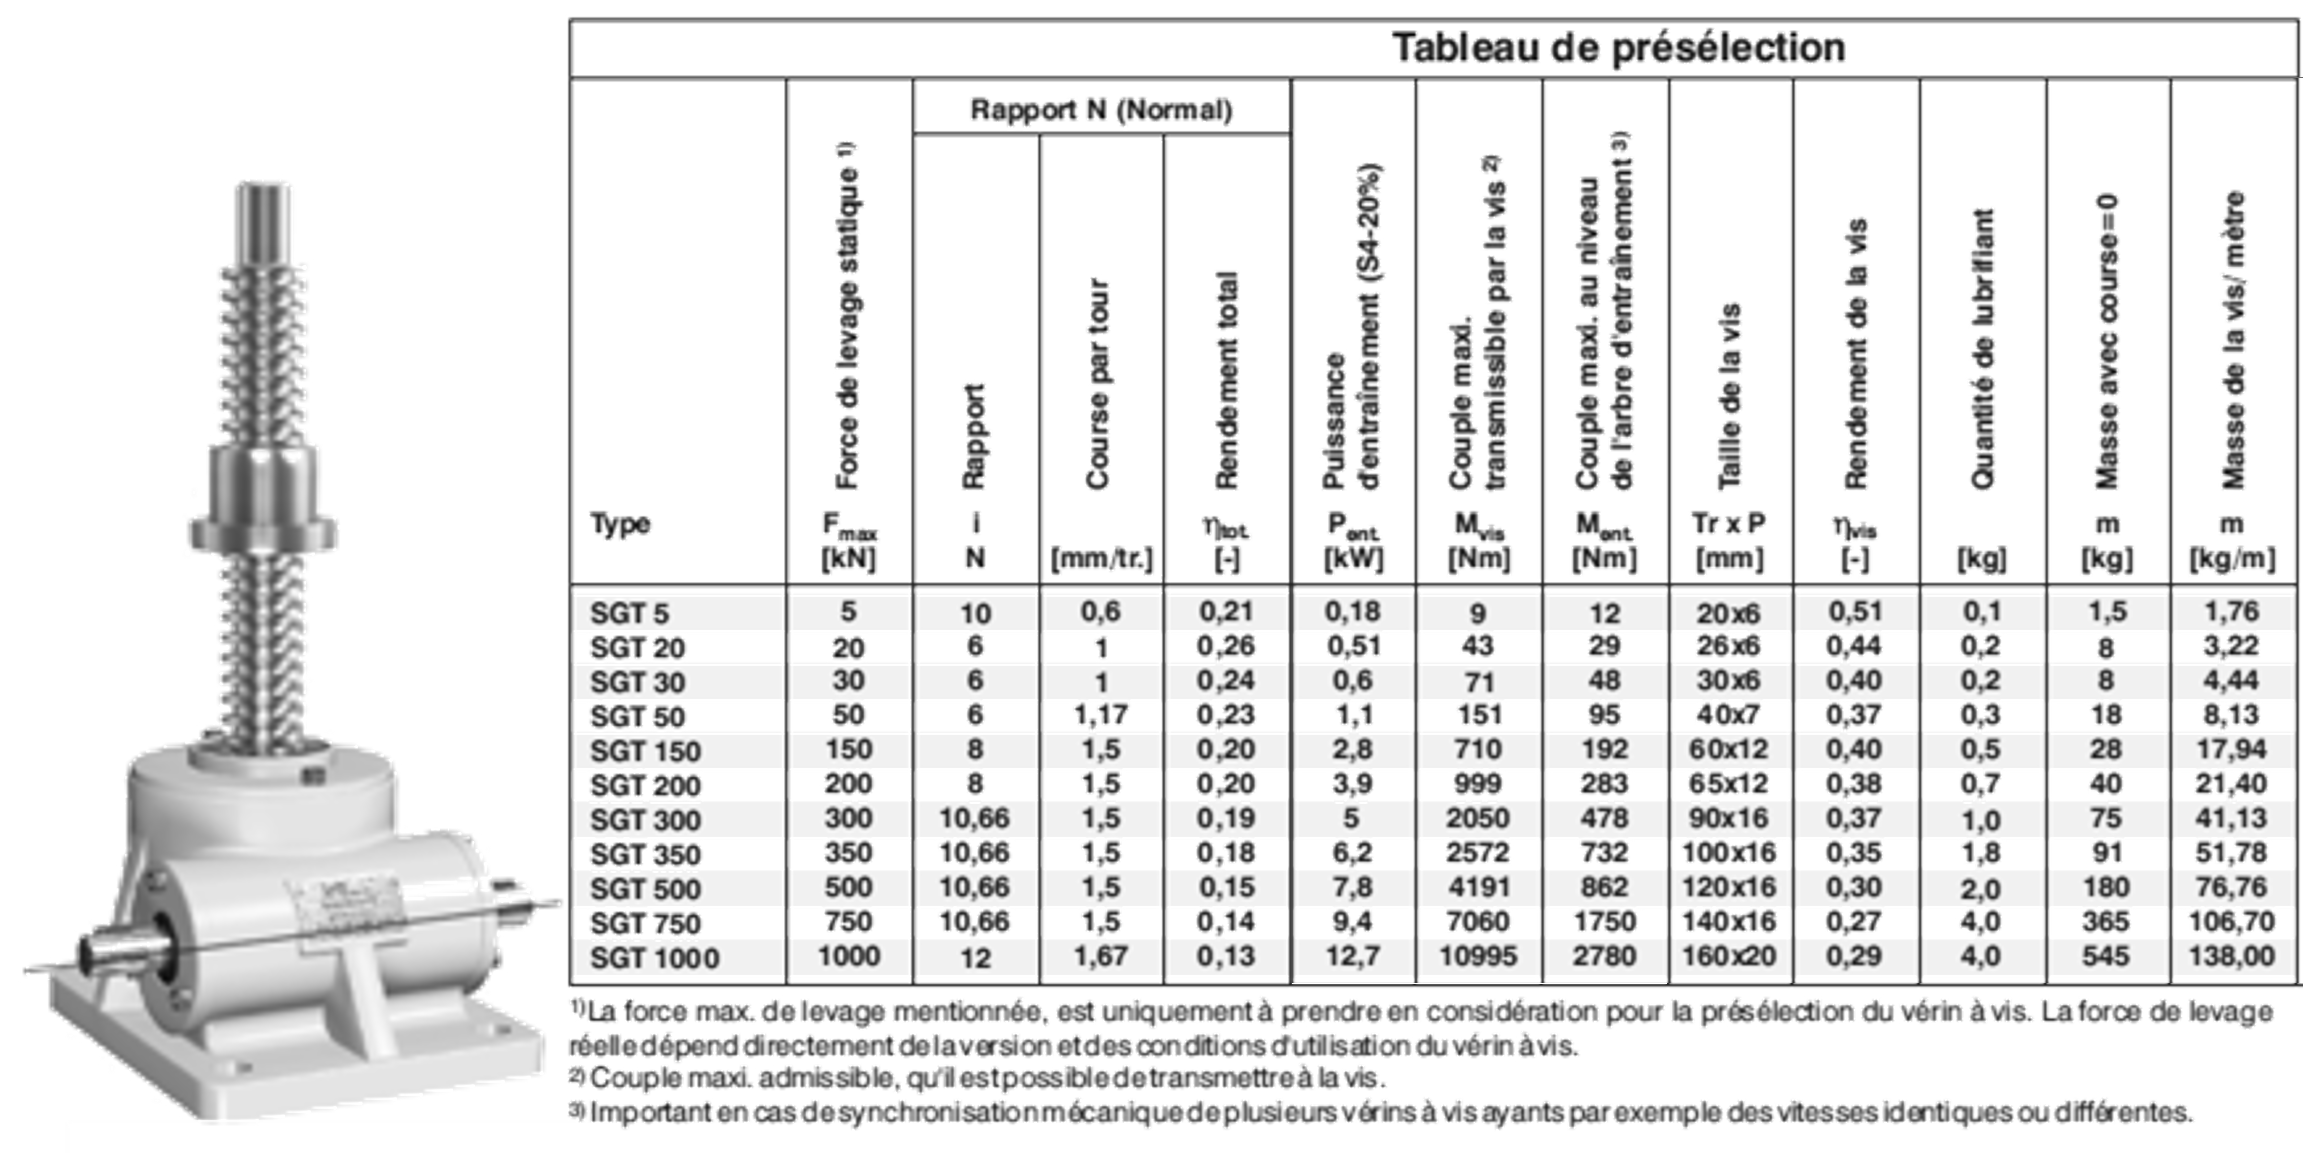
\includegraphics[width=0.8\linewidth]{img/fig6}
\caption{Vérins électriques}
\label{fig6}
\end{figure}

~\

\begin{figure}[!h]
\centering
\begin{minipage}{0.5\linewidth}
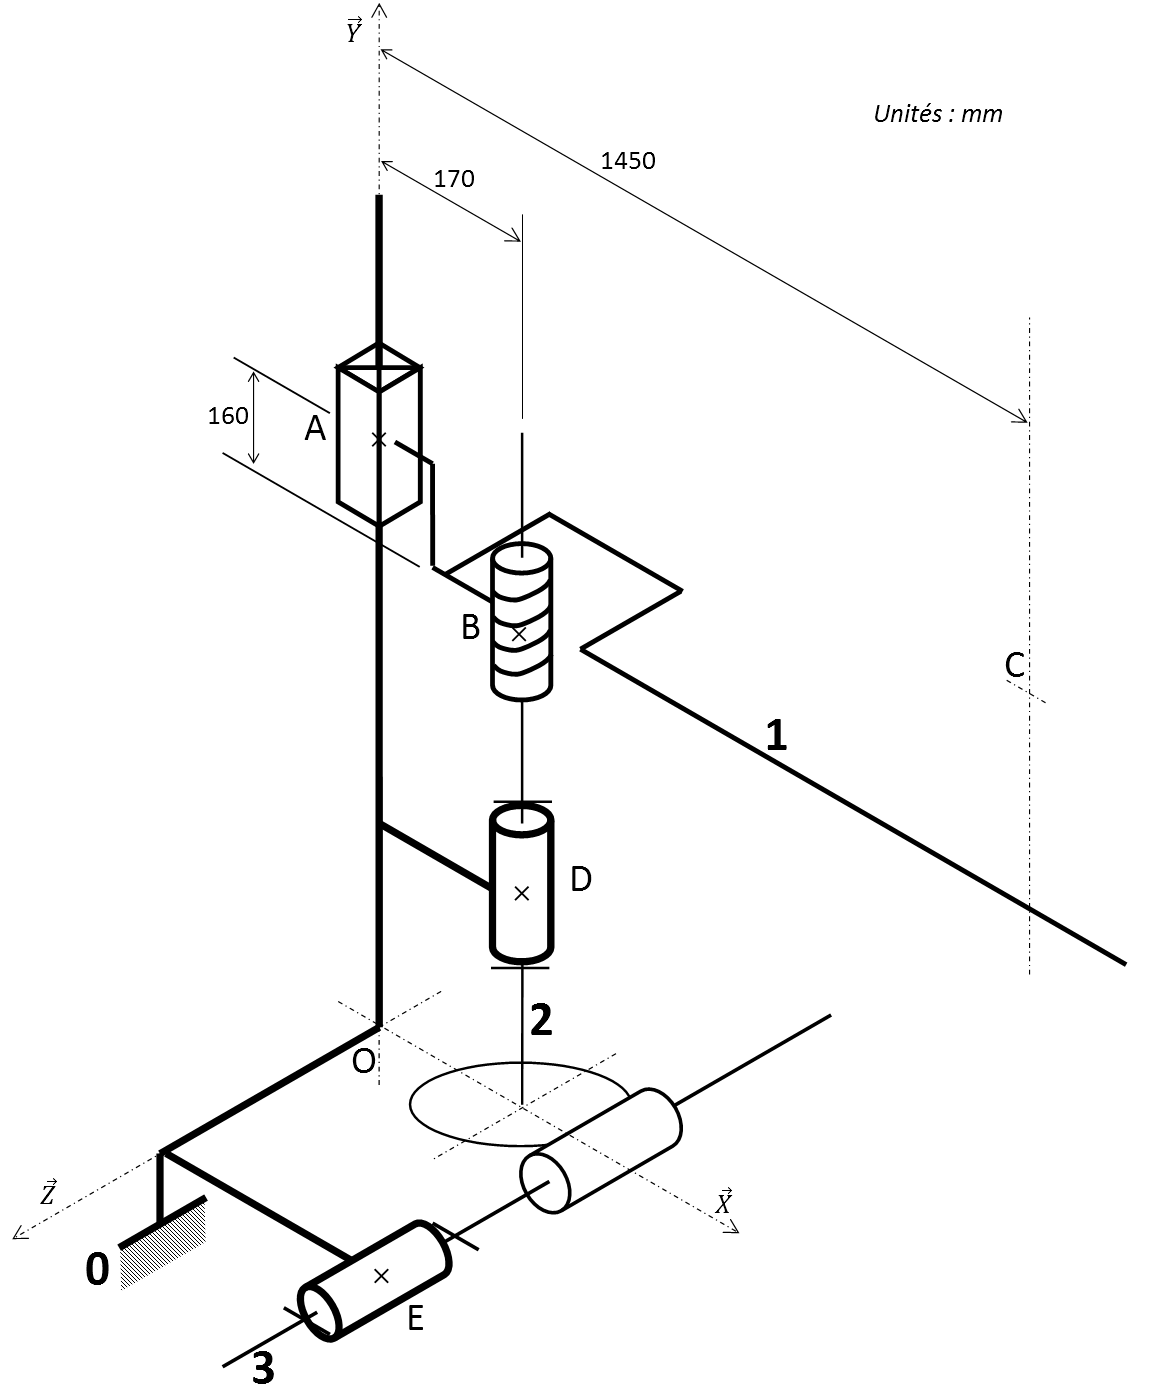
\includegraphics[width=0.8\linewidth]{img/fig8}
\caption{Schéma cinématique}
\label{fig8}
\end{minipage}\hfill
\begin{minipage}{0.45\linewidth}
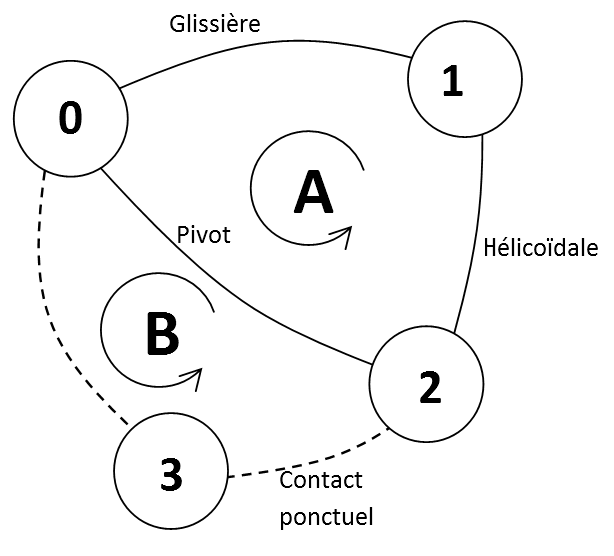
\includegraphics[width=\linewidth]{img/fig9}
\caption{Graphe des liaisons}
\label{fig9}
\end{minipage}
\end{figure}

~\

\begin{figure}[!h]
\centering
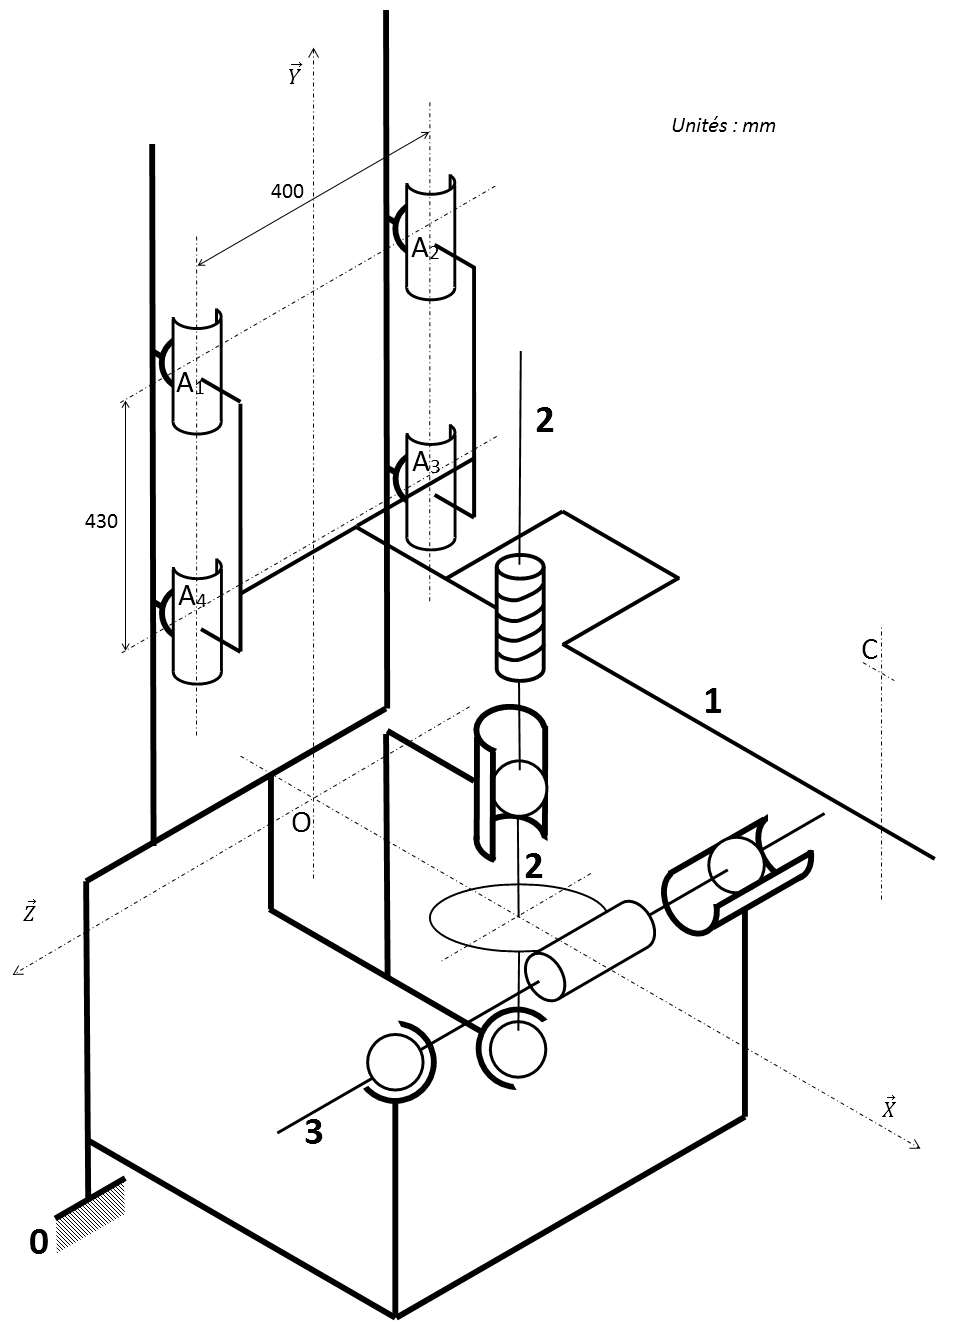
\includegraphics[width=0.55\linewidth]{img/fig10}
\caption{Schéma architectural}
\label{fig10}
\end{figure}

\newpage

Action transmissible dans la liaison glissière d'axe $(O,\overrightarrow{Y})$ réalisée par 4 douilles à billes:
\begin{center}
$\left\{T_{0\rightarrow 1}\right\}=\left\{\begin{array}{cc}X & L \\ 0 & M \\ Z & N\end{array}\right\}_{O,(\overrightarrow{X},\overrightarrow{Y},\overrightarrow{Z})}$
\end{center}

Chaque douille à billes est modélisable par une liaison sphère cylindre, soit
\begin{center}
$\left\{T_{0\rightarrow 1}\right\}_1=\left\{\begin{array}{cc}O_{1X} & 0 \\ 0 & 0 \\ O_{1Z} & 0\end{array}\right\}_{O_1,(\overrightarrow{X},\overrightarrow{Y},\overrightarrow{Z})}$,$\left\{T_{0\rightarrow 1}\right\}_2=\left\{\begin{array}{cc}O_{2X} & 0 \\ 0 & 0 \\ O_{2Z} & 0\end{array}\right\}_{O_2,(\overrightarrow{X},\overrightarrow{Y},\overrightarrow{Z})},$
\end{center}

\begin{center}
$\left\{T_{0\rightarrow 1}\right\}_3=\left\{\begin{array}{cc}O_{3X} & 0 \\ 0 & 0 \\ O_{3Z} & 0\end{array}\right\}_{O_3,(\overrightarrow{X},\overrightarrow{Y},\overrightarrow{Z})},\left\{T_{0\rightarrow 1}\right\}_4=\left\{\begin{array}{cc}O_{4X} & 0 \\ 0 & 0 \\ O_{4Z} & 0\end{array}\right\}_{O_4,(\overrightarrow{X},\overrightarrow{Y},\overrightarrow{Z})}$
\end{center}


\begin{figure}[!h]
\centering
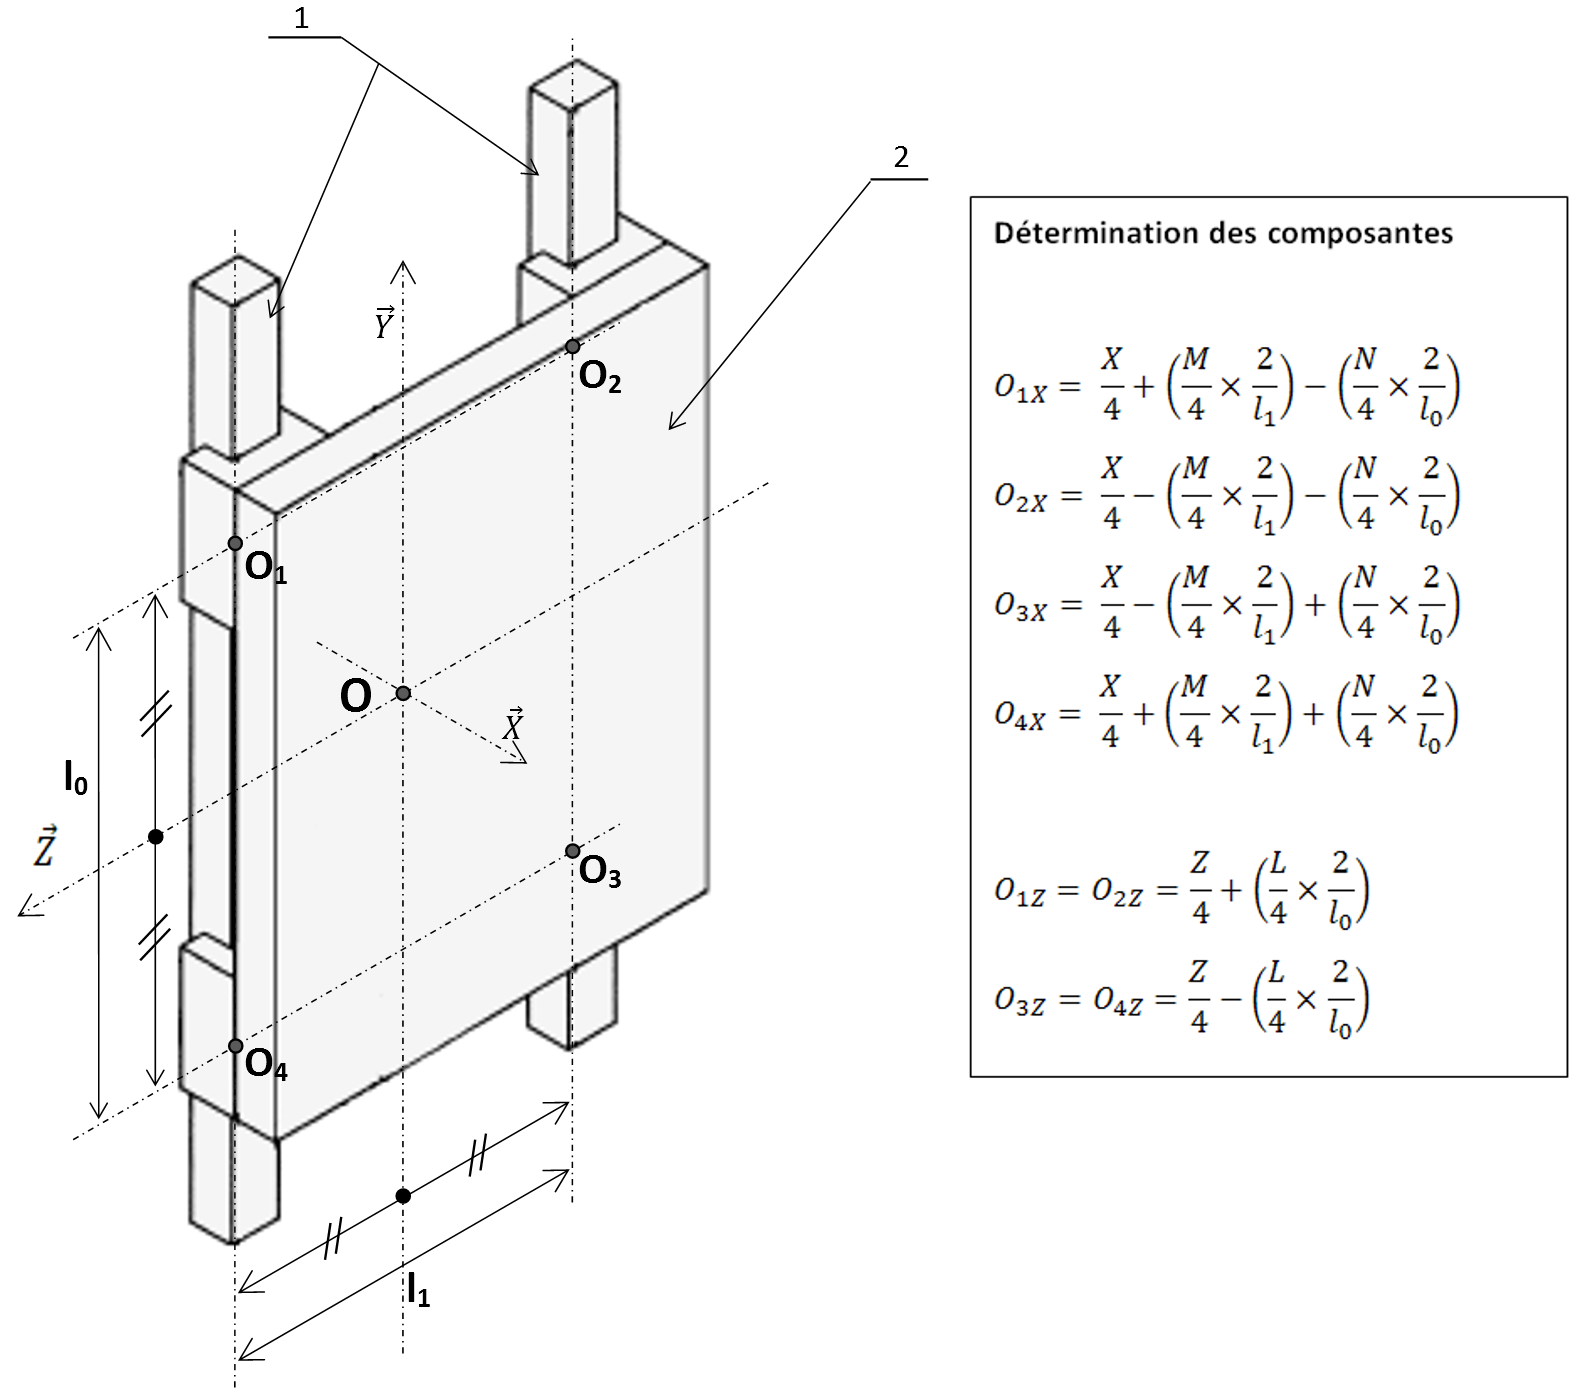
\includegraphics[width=0.6\linewidth]{img/fig11}
\caption{Détermination des charges radiales dans les douilles à billes}
\label{fig11}
\end{figure}

\cleardoublepage

\section{Document réponse}

\lhead{Nom:................. Prénom:...............}

\reponse{1}{0}

\begin{center}
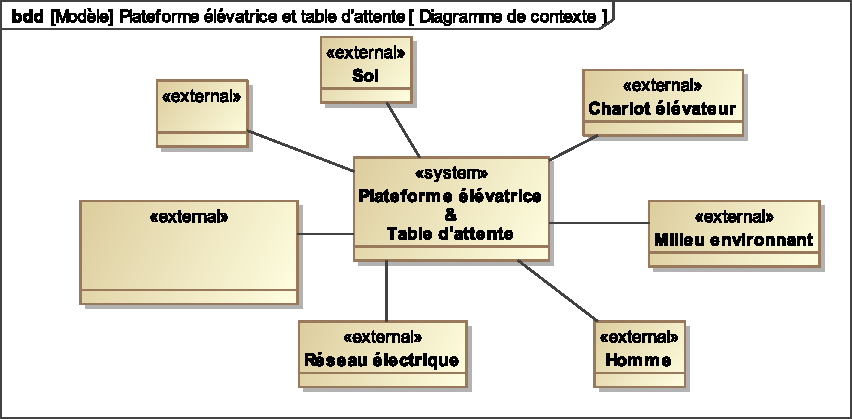
\includegraphics[width=0.95\linewidth]{img/Diagramme_de_contexte_vide}
\end{center}

\reponse{2}{4}

\reponse{3}{6}

\reponse{4}{3}

\reponse{5}{6}

\reponse{6}{12}

\reponse{7}{12}

\reponse{8}{12}

\reponse{9}{14}

\reponse{10}{13}

\cleardoublepage

\reponse{11}{1}

\begin{center}
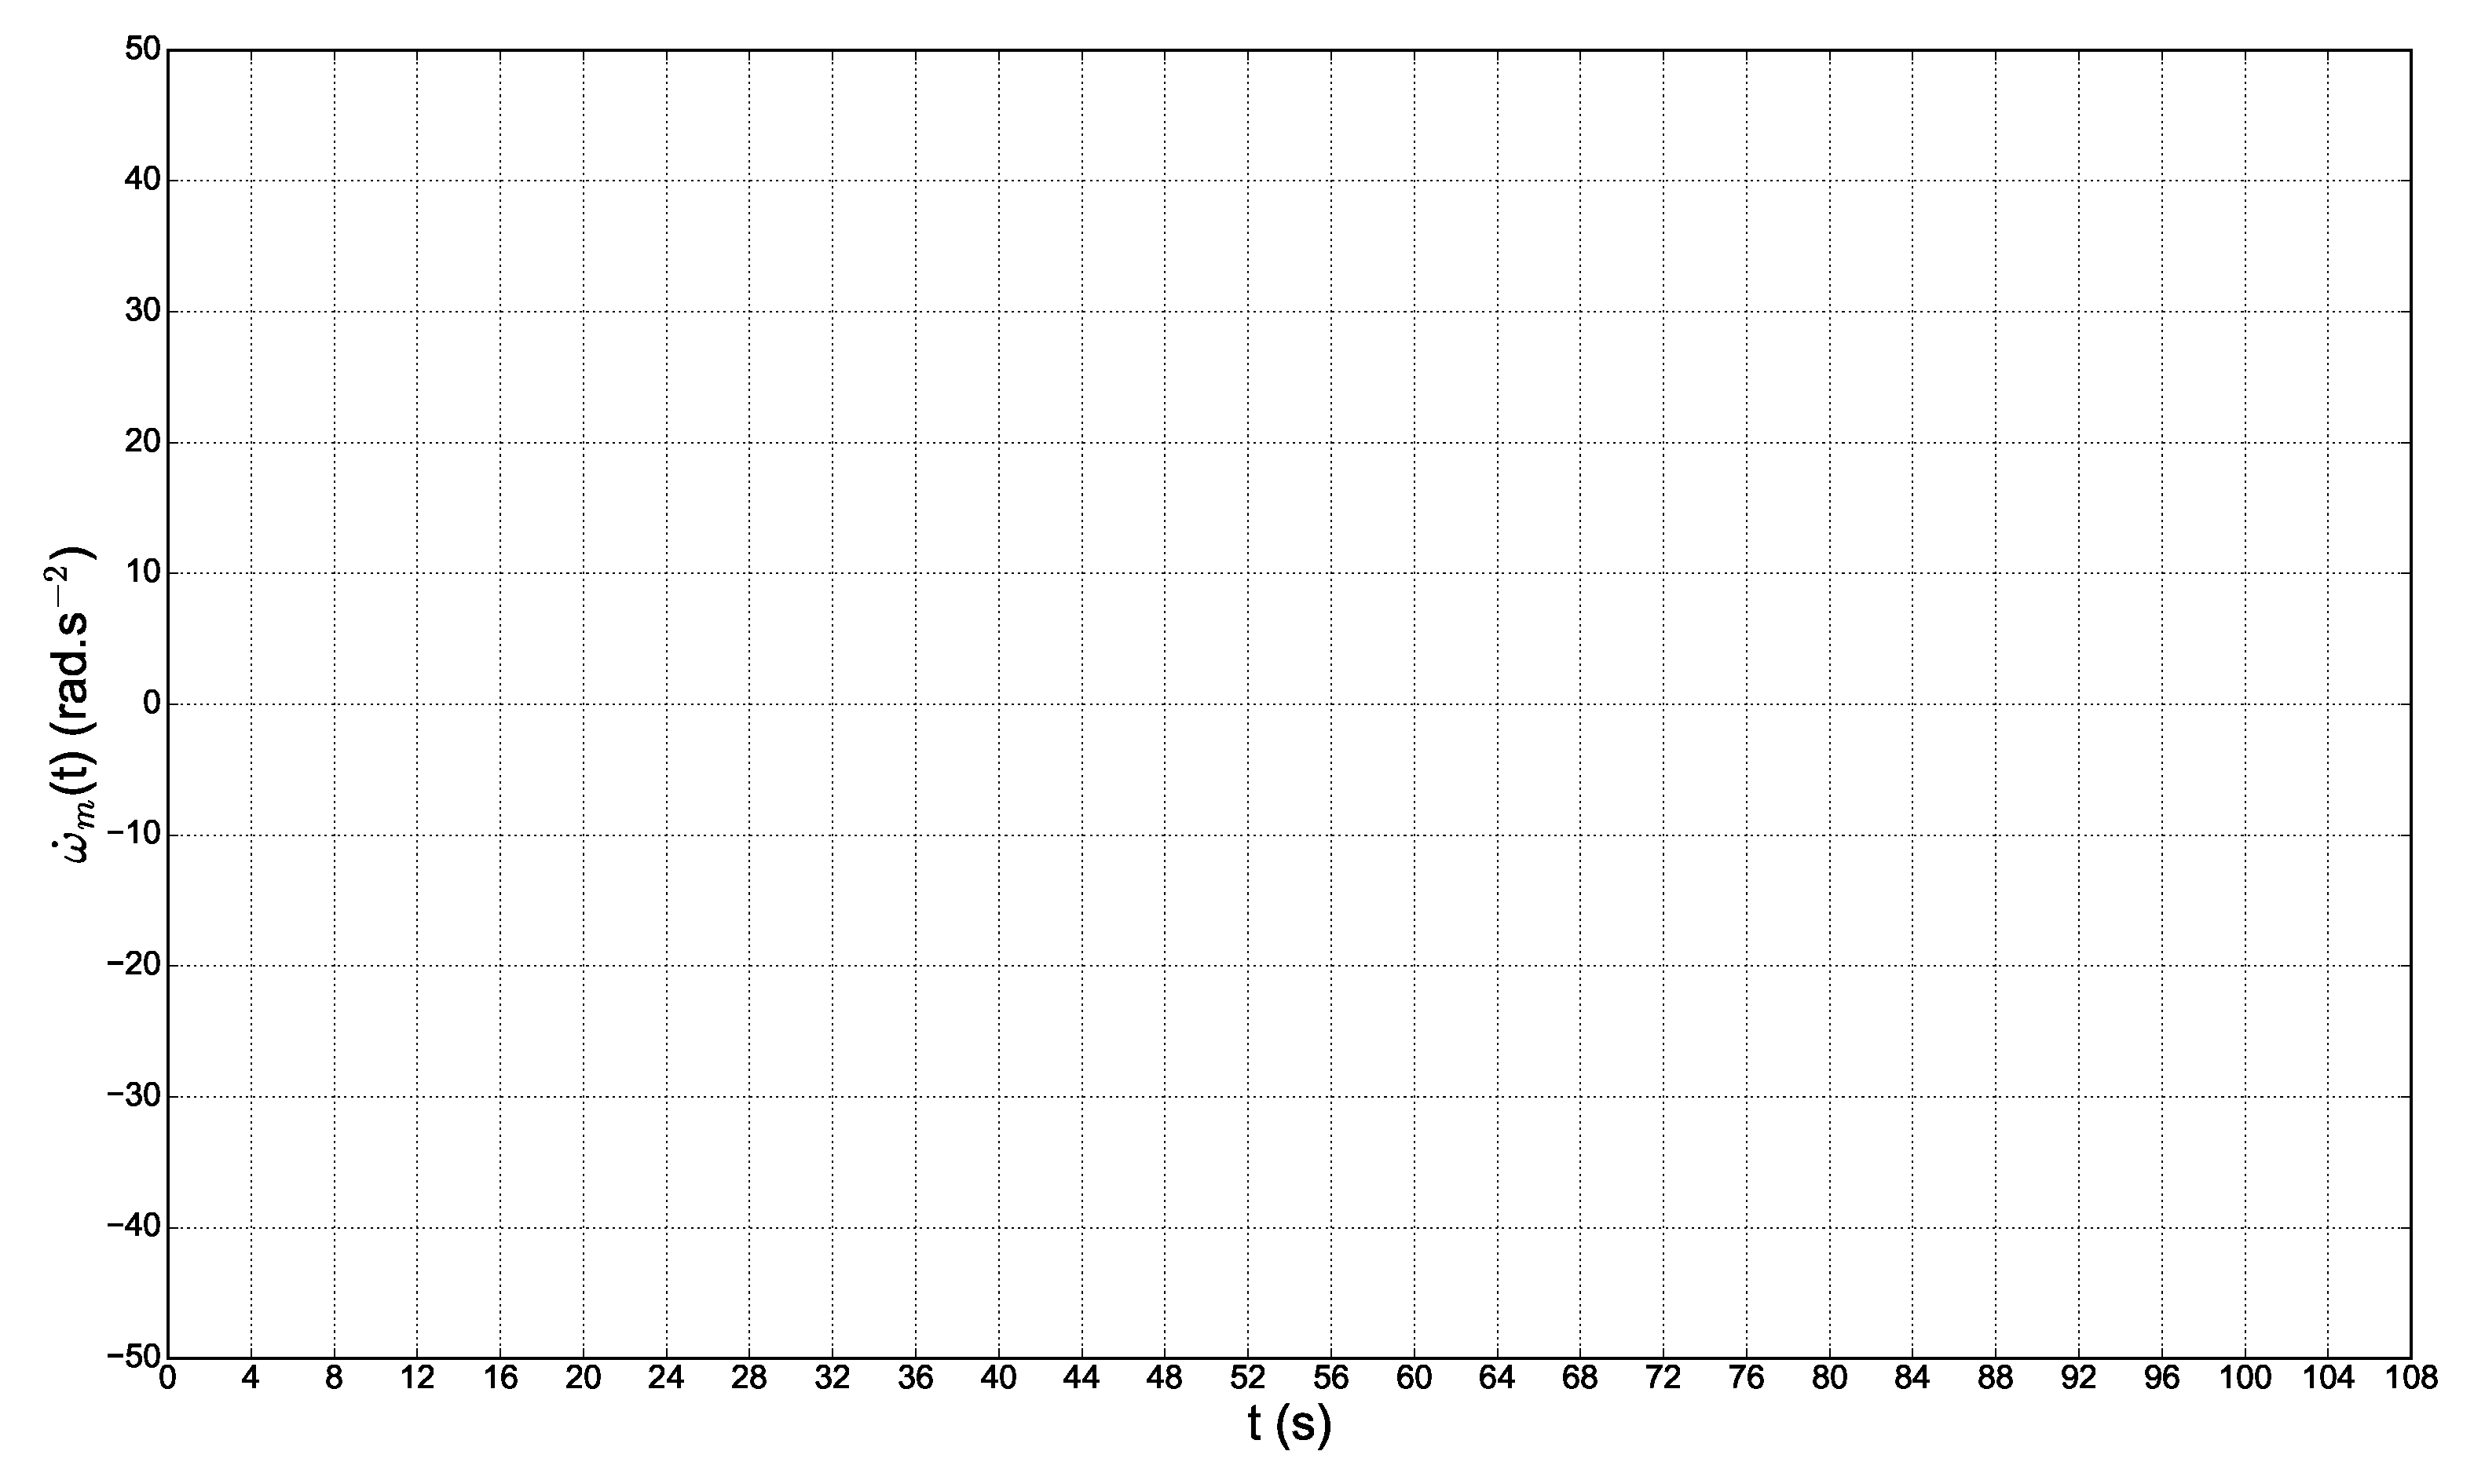
\includegraphics[width=0.95\linewidth]{img/accel}
\end{center}

\reponse{12}{1}

\begin{center}
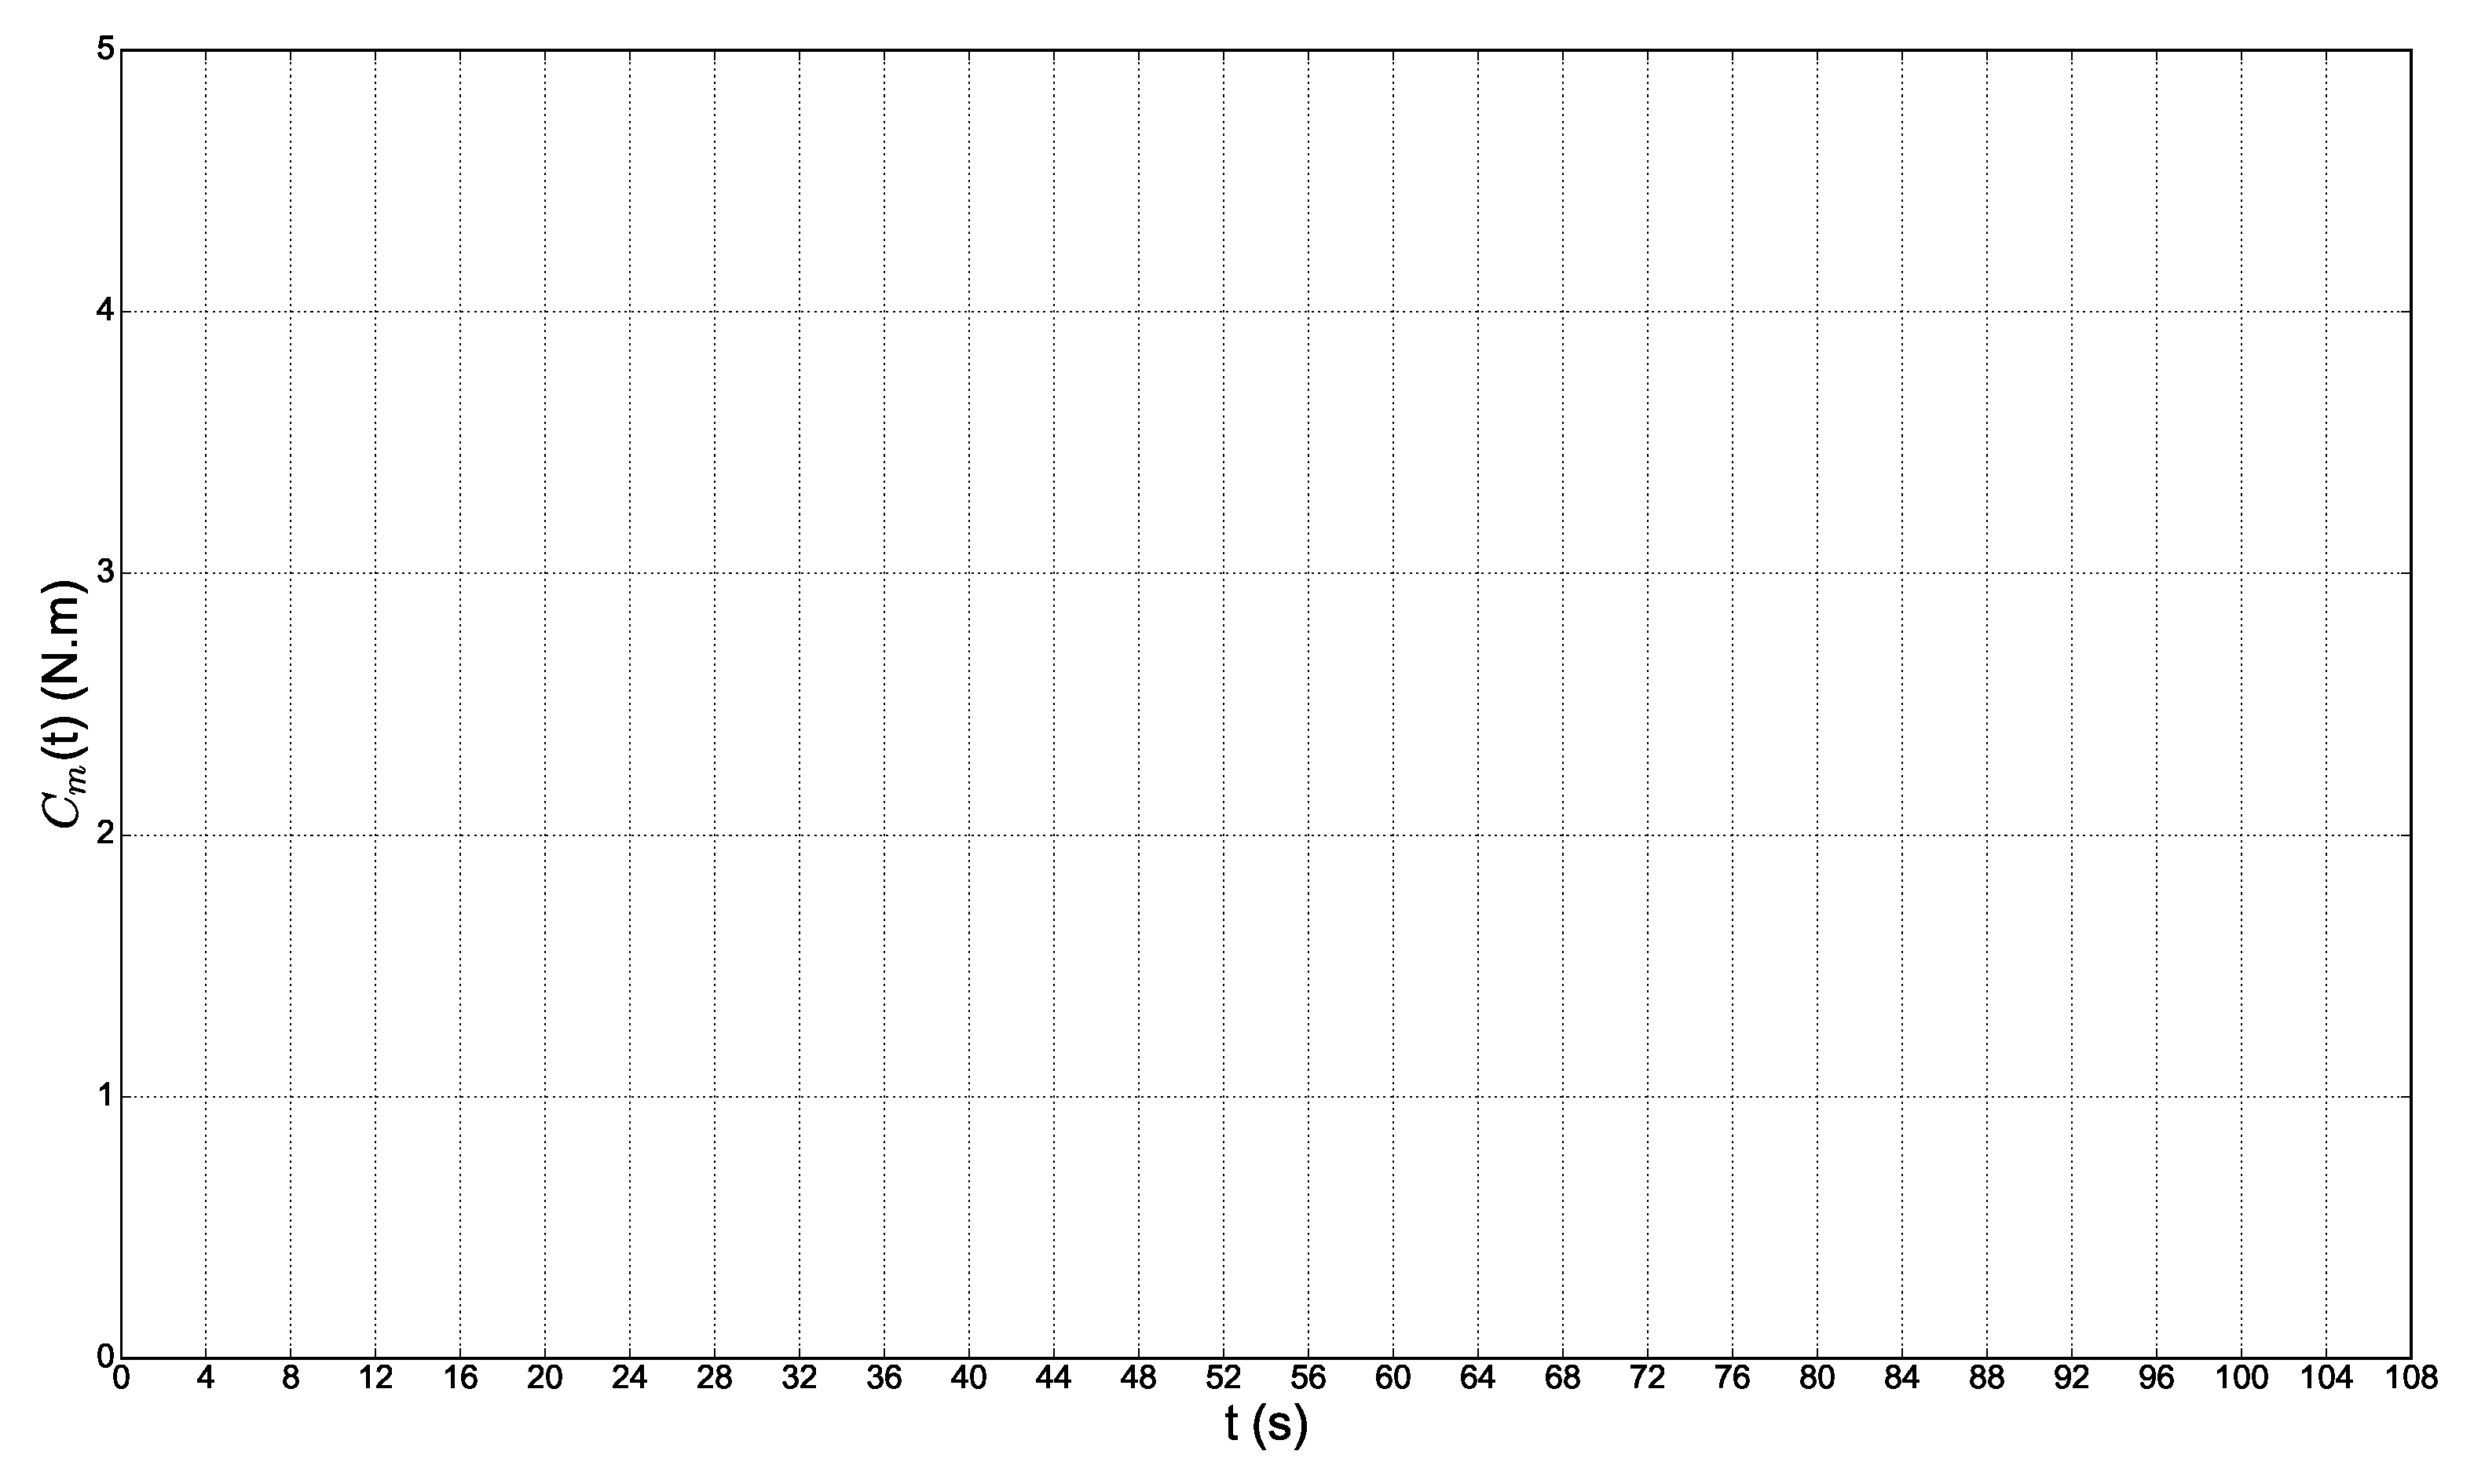
\includegraphics[width=0.95\linewidth]{img/couple}
\end{center}

\reponse{13}{5}

\reponse{14}{1}

\begin{center}
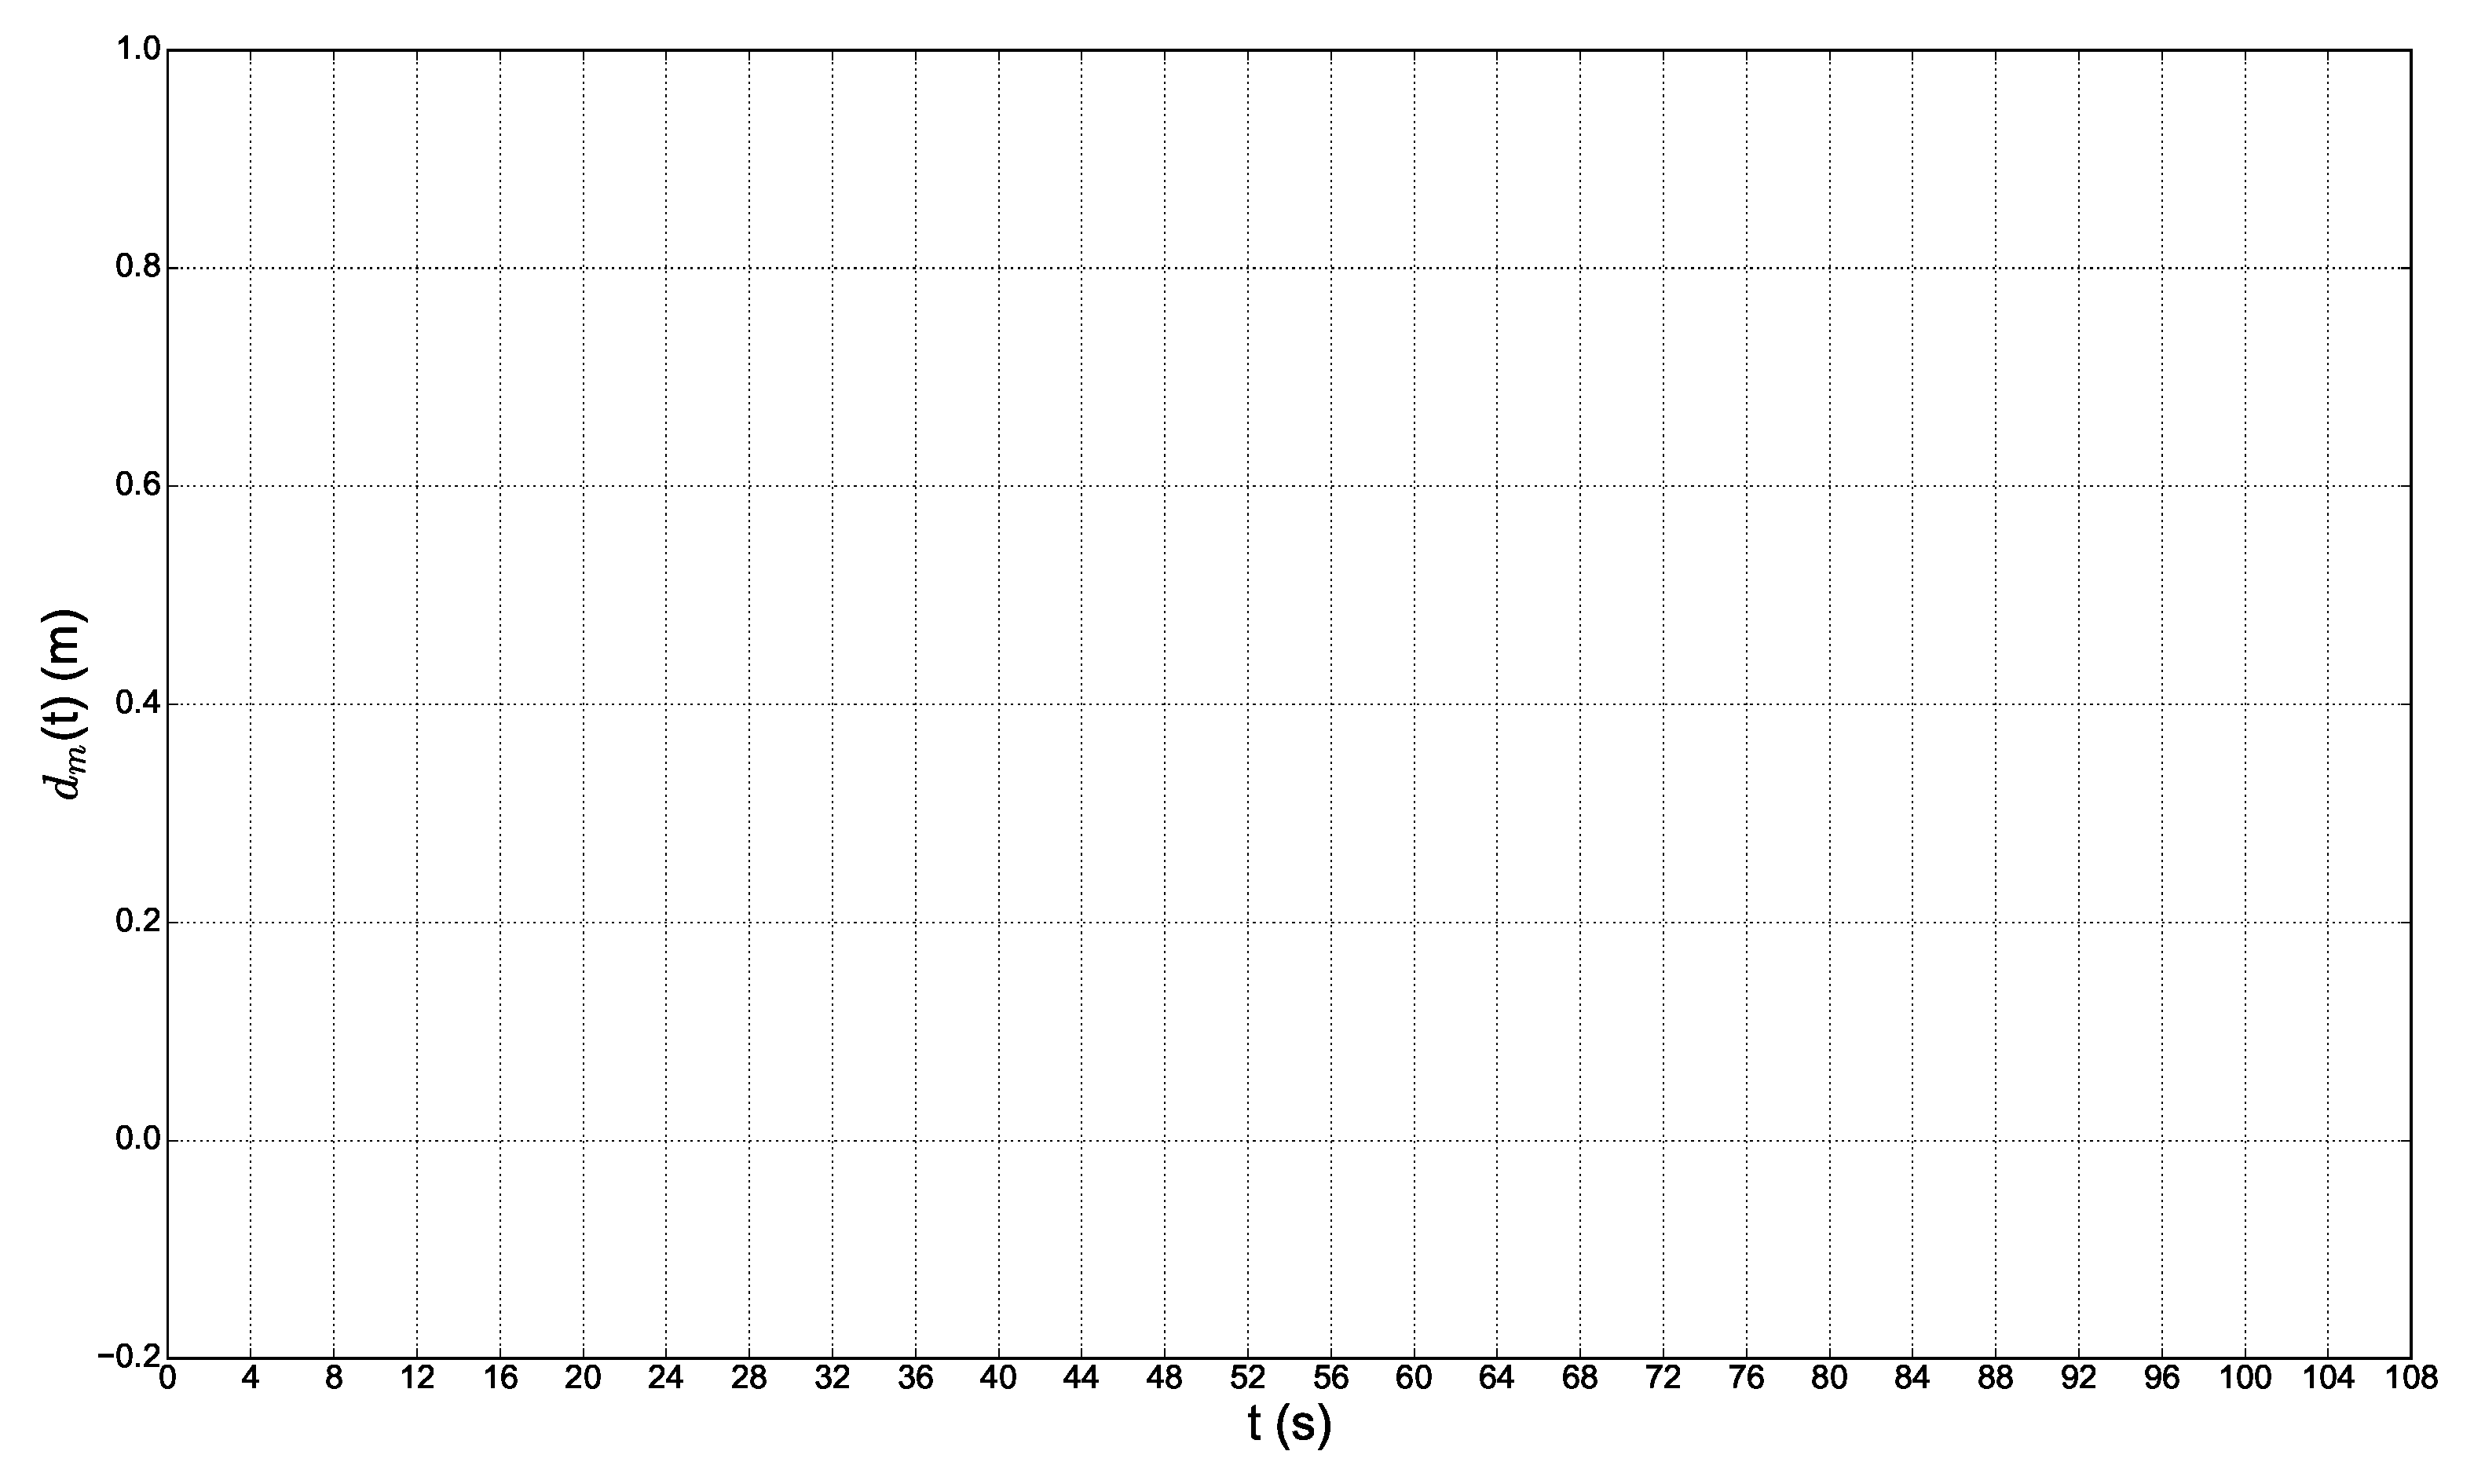
\includegraphics[width=0.95\linewidth]{img/deplacement}
\end{center}

\reponse{15}{5}

\reponse{16}{6}

\reponse{17}{5}

\reponse{18}{5}

\reponse{19}{2}

\begin{center}
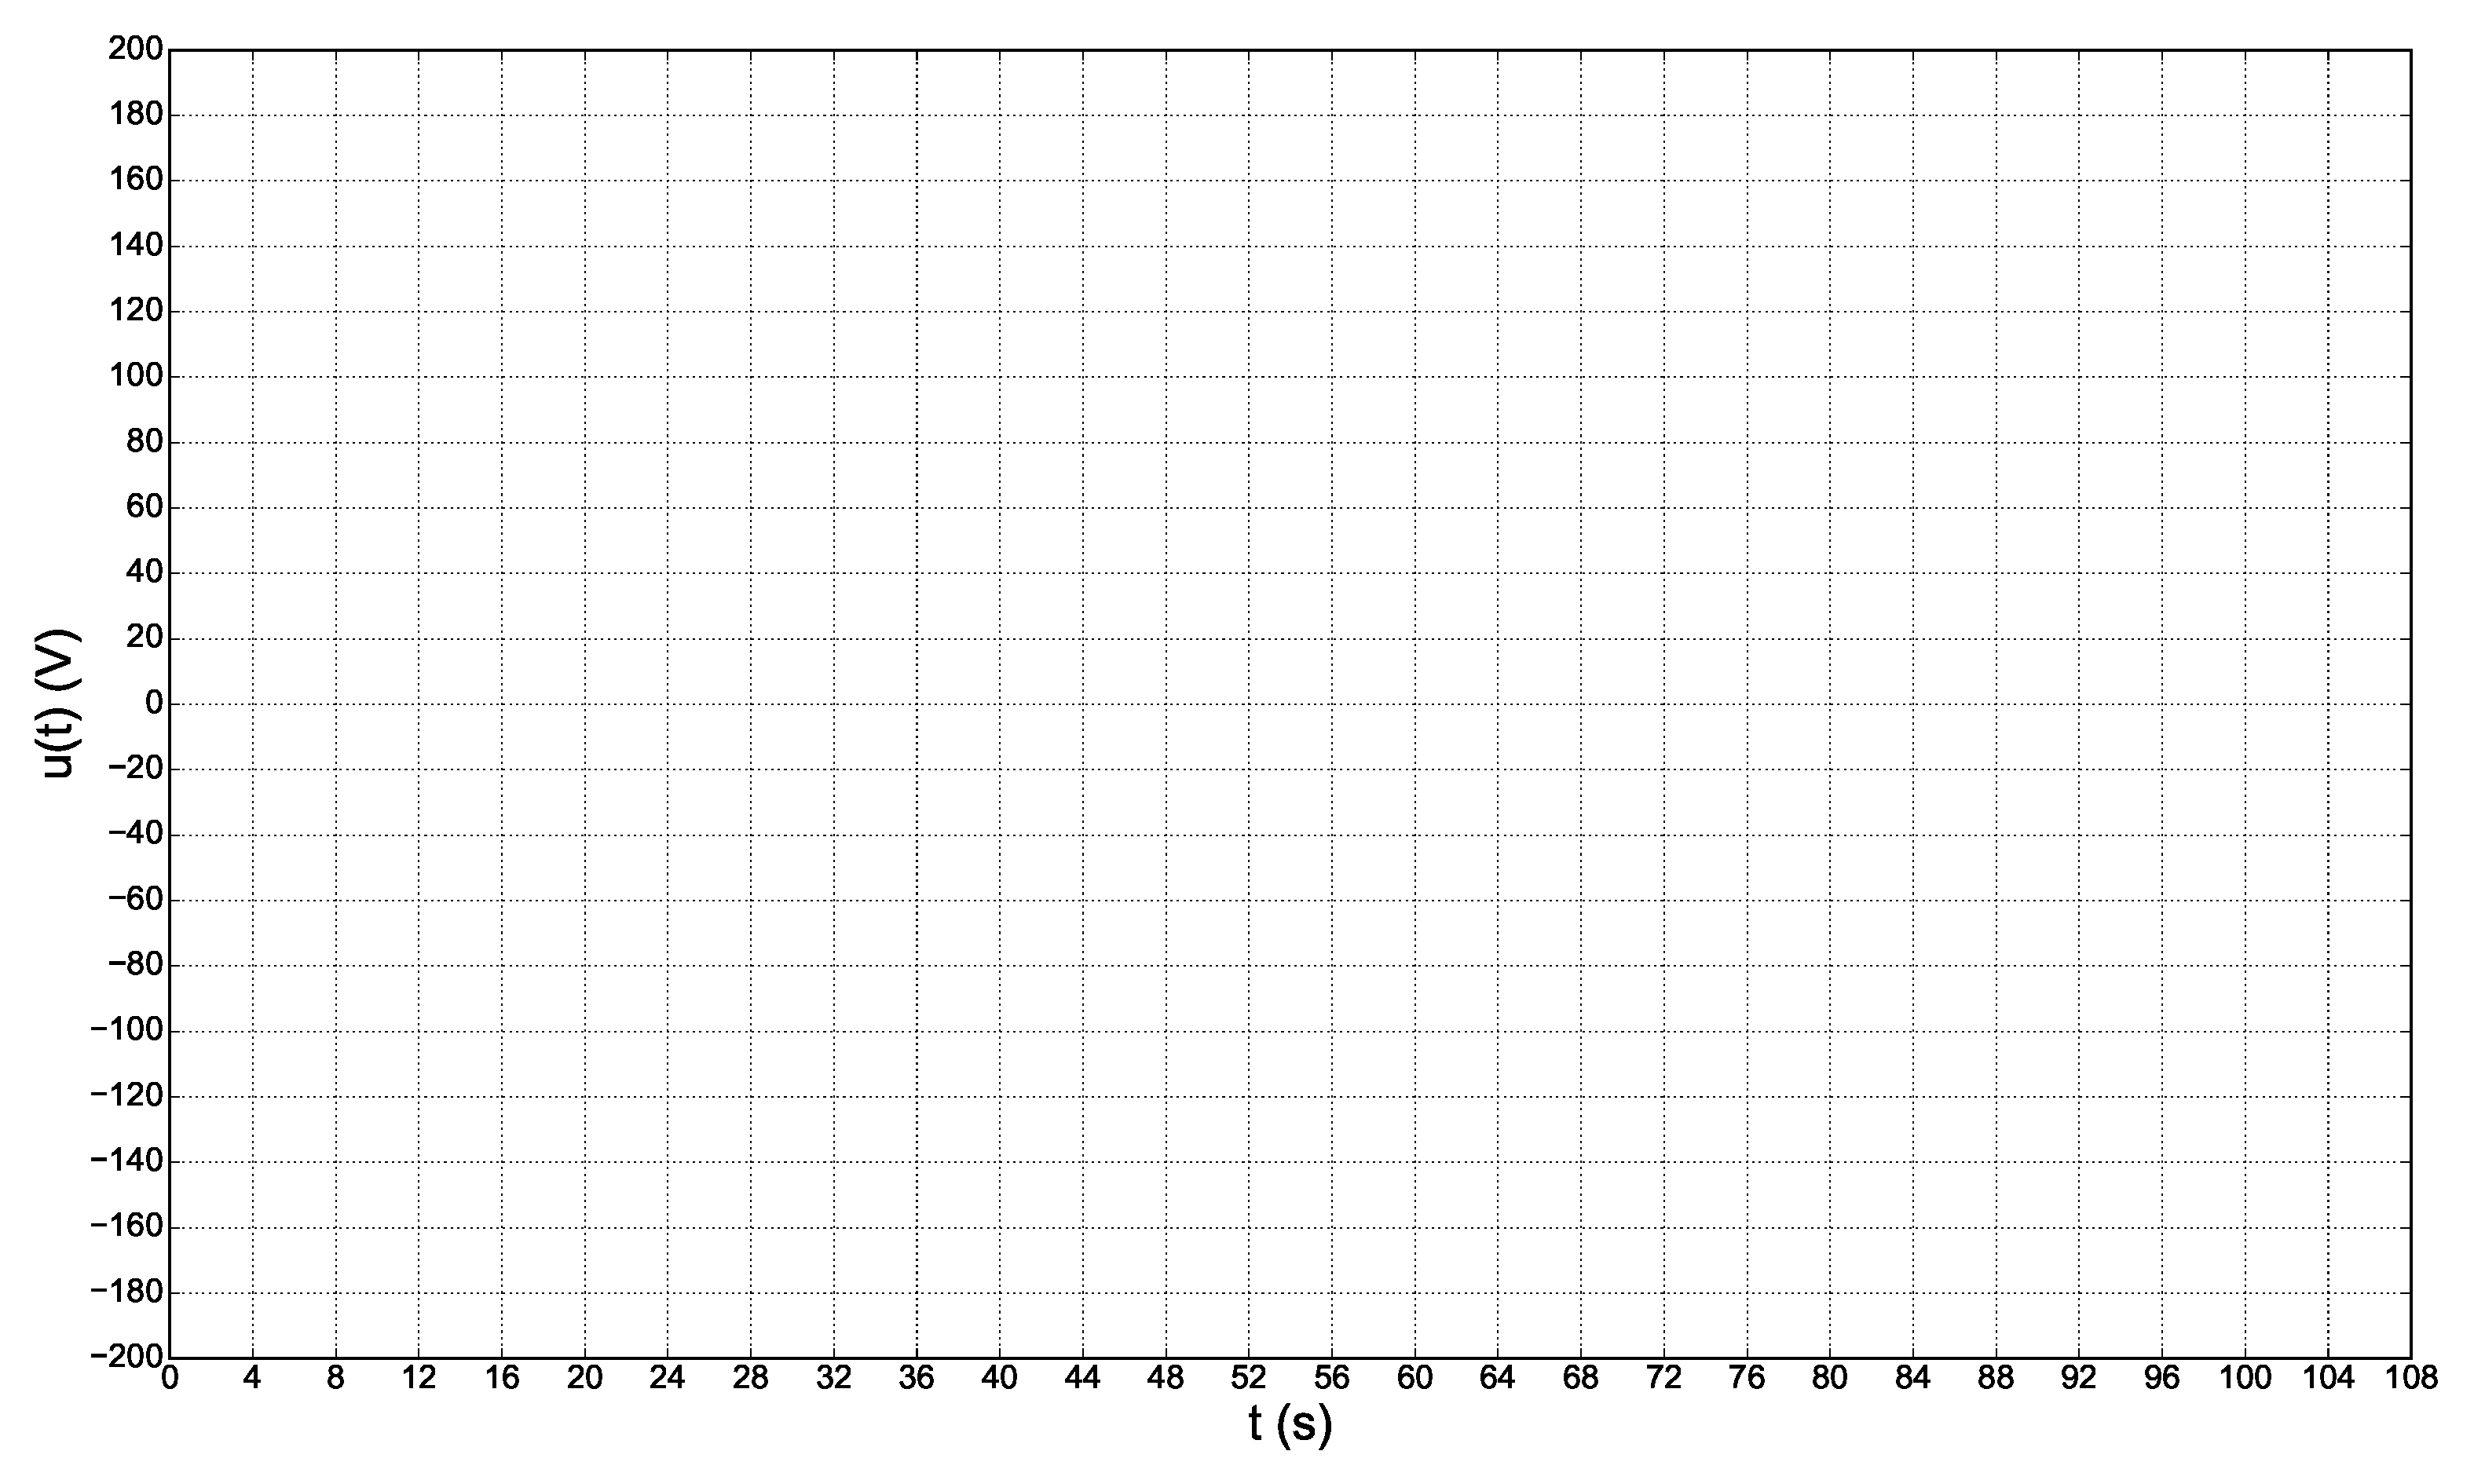
\includegraphics[width=0.95\linewidth]{img/tension}
\end{center}

\reponse{20}{5}

\reponse{21}{5}

\reponse{22}{5}


\ifdef{\public}{\end{document}}{}

\newpage
\cleardoublepage

\pagestyle{correction}

\section{Correction}

\reponse{1}{0}

\begin{center}
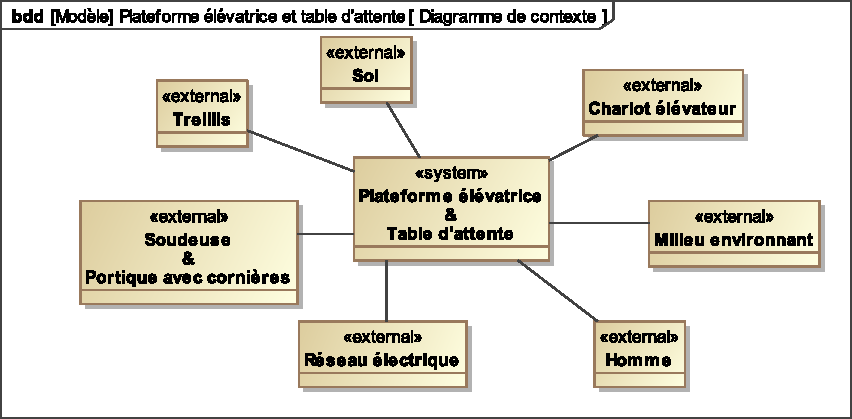
\includegraphics[width=0.95\linewidth]{img/Diagramme_de_contexte}
\end{center}

\reponse{2}{0}

$nb=5\times11\times44\times0,95\times60=137940$ treillis par an.

\reponse{3}{0}

$\left\{\begin{array}{l}
r_s = 6.(p-1)- m_c \\
r_s = 6\times 2 - 1 = 11 \\
I_s = 5 + 5 + 5 = 15 \\
h=I_s-r_s = 4\end{array}\right. \rightarrow$ hyperstatique de degré 4.

\reponse{4}{0}

On peut mettre du jeu dans la liaison hélicoïdale ou mettre un système de réglage.

\reponse{5}{0}

On veut réaliser une glissière (5 inconnues statiques) par 4 linéaires annulaires (2 inconnues
statiques / liaison).

$\left\{\begin{array}{l}
r_s = 6.(p-1)- m_c = 11 \\
r_s = 6\times 1 - 1 = 5 \\
I_s = 4\times 2 = 8 \\
h=I_s-r_s = 3\end{array}\right. \rightarrow$ hyperstatique de degré 3.

\reponse{6}{0}

Le rapport est de $6$ et la course par tour est de $1,17mm/tr$, on a donc un pas de $6*1,17=7mm$.

\reponse{7}{0}

Bilan des actions :

\begin{itemize}
 \item Action du poids: $\left\{T_{g\rightarrow 1}\right\}=\left\{\begin{array}{cc}0 & 0 \\ Y_{Cg\rightarrow 1} & 0 \\ 0 & 0\end{array}\right\}_{C,(\overrightarrow{X},\overrightarrow{Y},\overrightarrow{Z})}$, avec $Y_{Cg\rightarrow 1}=-5000N$,
 \item Action de la vis (2): $\left\{T_{2\rightarrow 1}\right\}=\left\{\begin{array}{cc}0 & 0 \\ Y_{B2\rightarrow 1} & M_{B2\rightarrow 1} \\ 0 & 0\end{array}\right\}_{B,(\overrightarrow{X},\overrightarrow{Y},\overrightarrow{Z})}$,
  \item Action du bâti (0): $\left\{T_{0\rightarrow 1}\right\}=\left\{\begin{array}{cc}X_{A0\rightarrow 1} & L_{A0\rightarrow 1} \\ 0 & M_{A0\rightarrow 1} \\ Z_{A0\rightarrow 1} & N_{A0\rightarrow 1}\end{array}\right\}_{A	,(\overrightarrow{X},\overrightarrow{Y},\overrightarrow{Z})}$.
 \end{itemize}

\reponse{8}{0}

Écriture des torseurs en A

\begin{itemize}
 \item Action du poids: $\left\{T_{g\rightarrow 1}\right\}=\left\{\begin{array}{cc}0 & 0 \\ Y_{Cg\rightarrow 1} & 0 \\ 0 & 1450.Y_{Cg\rightarrow 1}\end{array}\right\}_{A,(\overrightarrow{X},\overrightarrow{Y},\overrightarrow{Z})}$, avec $Y_{Cg\rightarrow 1}=-5000N$,
 \item Action de la vis (2): $\left\{T_{2\rightarrow 1}\right\}=\left\{\begin{array}{cc}0 & 0 \\ Y_{B2\rightarrow 1} & M_{B2\rightarrow 1} \\ 0 & 170.Y_{B2\rightarrow 1}\end{array}\right\}_{A,(\overrightarrow{X},\overrightarrow{Y},\overrightarrow{Z})}$.
 \end{itemize}

$\left\{\begin{array}{l}
X_{A0\rightarrow 1}+0+0=0 \\
0+Y_{Cg\rightarrow 1}+Y_{B2\rightarrow 1}=0 \\
Z_{A0\rightarrow 1}+0+0=0 \\
L_{A0\rightarrow 1}+0+0=0 \\
M_{A0\rightarrow 1}+M_{B2\rightarrow 1}+0=0 \\
X_{A0\rightarrow 1}+1450.Y_{Cg\rightarrow 1}+170.Y_{B2\rightarrow 1}=0
\end{array}\right.$, avec $M_{B2\rightarrow 1}=0,0035(ou\ 0,0012).Y_{B2\rightarrow 1}$

\reponse{9}{0}

Ainsi,

$\left\{\begin{array}{l}
Y_{B2\rightarrow 1}=-Y_{Cg\rightarrow 1}=5000N \\
M_{B2\rightarrow 1}=0,0035.5000=17,5N.m \text{ vis trapézoïdale}\\
M_{B2\rightarrow 1}=0,0012.5000=6N.m \text{ vis à billes}\\
X_{A0\rightarrow 1}=0 \\
Z_{A0\rightarrow 1}=0 \\
L_{A0\rightarrow 1}=0 \\
M_{A0\rightarrow 1}=-M_{B2\rightarrow 1} \\
N_{A0\rightarrow 1}=1450.Y_{Cg\rightarrow 1}-170.Y_{B2\rightarrow 1}=(170-1450).5000=6400N.m
\end{array}\right.$

Conclusion
\begin{itemize}
  \item Action du bâti (vis trapézoïdale): $\left\{T_{0\rightarrow 1}\right\}=\left\{\begin{array}{cc}0 & 0 \\ 0 & -17,5 \\ 0 & 6400\end{array}\right\}_{A	,(\overrightarrow{X},\overrightarrow{Y},\overrightarrow{Z})}$,
  \item Action du bâti (vis à billes): $\left\{T_{0\rightarrow 1}\right\}=\left\{\begin{array}{cc}0 & 0 \\ 0 & -6 \\ 0 & 6400\end{array}\right\}_{A	,(\overrightarrow{X},\overrightarrow{Y},\overrightarrow{Z})}$.
 \end{itemize}
 
\reponse{10}{0}

D'après le document 3 : $l_0=0,43m$ et $l_1=0,4m$.

En utilisant le document 4, on déduit :
\begin{itemize}
 \item Pour une vis trapézoïdale:
 \begin{itemize}
  \item $O_{1X}=\left(\frac{-17,5}{4}\times\frac{2}{0,4}\right)-\left(\frac{6400}{4}\times\frac{2}{0,43}\right)=-7464N$,
  \item $O_{2X}=-\left(\frac{-17,5}{4}\times\frac{2}{0,4}\right)-\left(\frac{6400}{4}\times\frac{2}{0,43}\right)=-7420N$,
  \item $O_{3X}=-\left(\frac{-17,5}{4}\times\frac{2}{0,4}\right)+\left(\frac{6400}{4}\times\frac{2}{0,43}\right)=7464N$,
  \item $O_{4X}=\left(\frac{-17,5}{4}\times\frac{2}{0,4}\right)+\left(\frac{6400}{4}\times\frac{2}{0,43}\right)=7420N$,
  \item $O_{1Z}=O_{2Z}=O_{3Z}=O_{4Z}=0$.
 \end{itemize}
 \item Pour une vis à billes:
 \begin{itemize}
  \item $O_{1X}=\left(\frac{-6}{4}\times\frac{2}{0,4}\right)-\left(\frac{6400}{4}\times\frac{2}{0,43}\right)=-7449N$,
  \item $O_{2X}=-\left(\frac{-6}{4}\times\frac{2}{0,4}\right)-\left(\frac{6400}{4}\times\frac{2}{0,43}\right)=-7449N$,
  \item $O_{3X}=-\left(\frac{-6}{4}\times\frac{2}{0,4}\right)+\left(\frac{6400}{4}\times\frac{2}{0,43}\right)=7449N$,
  \item $O_{4X}=\left(\frac{-6}{4}\times\frac{2}{0,4}\right)+\left(\frac{6400}{4}\times\frac{2}{0,43}\right)=7434N$,
  \item $O_{1Z}=O_{2Z}=O_{3Z}=O_{4Z}=0$.
 \end{itemize}
\end{itemize}

Dans tous les cas on a : $\sqrt{O_{iX}^2+O_{iZ}^2}<C_0$. Les douilles sont donc bien dimensionnées d'un point de vue statique.

\reponse{11}{0}

\begin{center}
 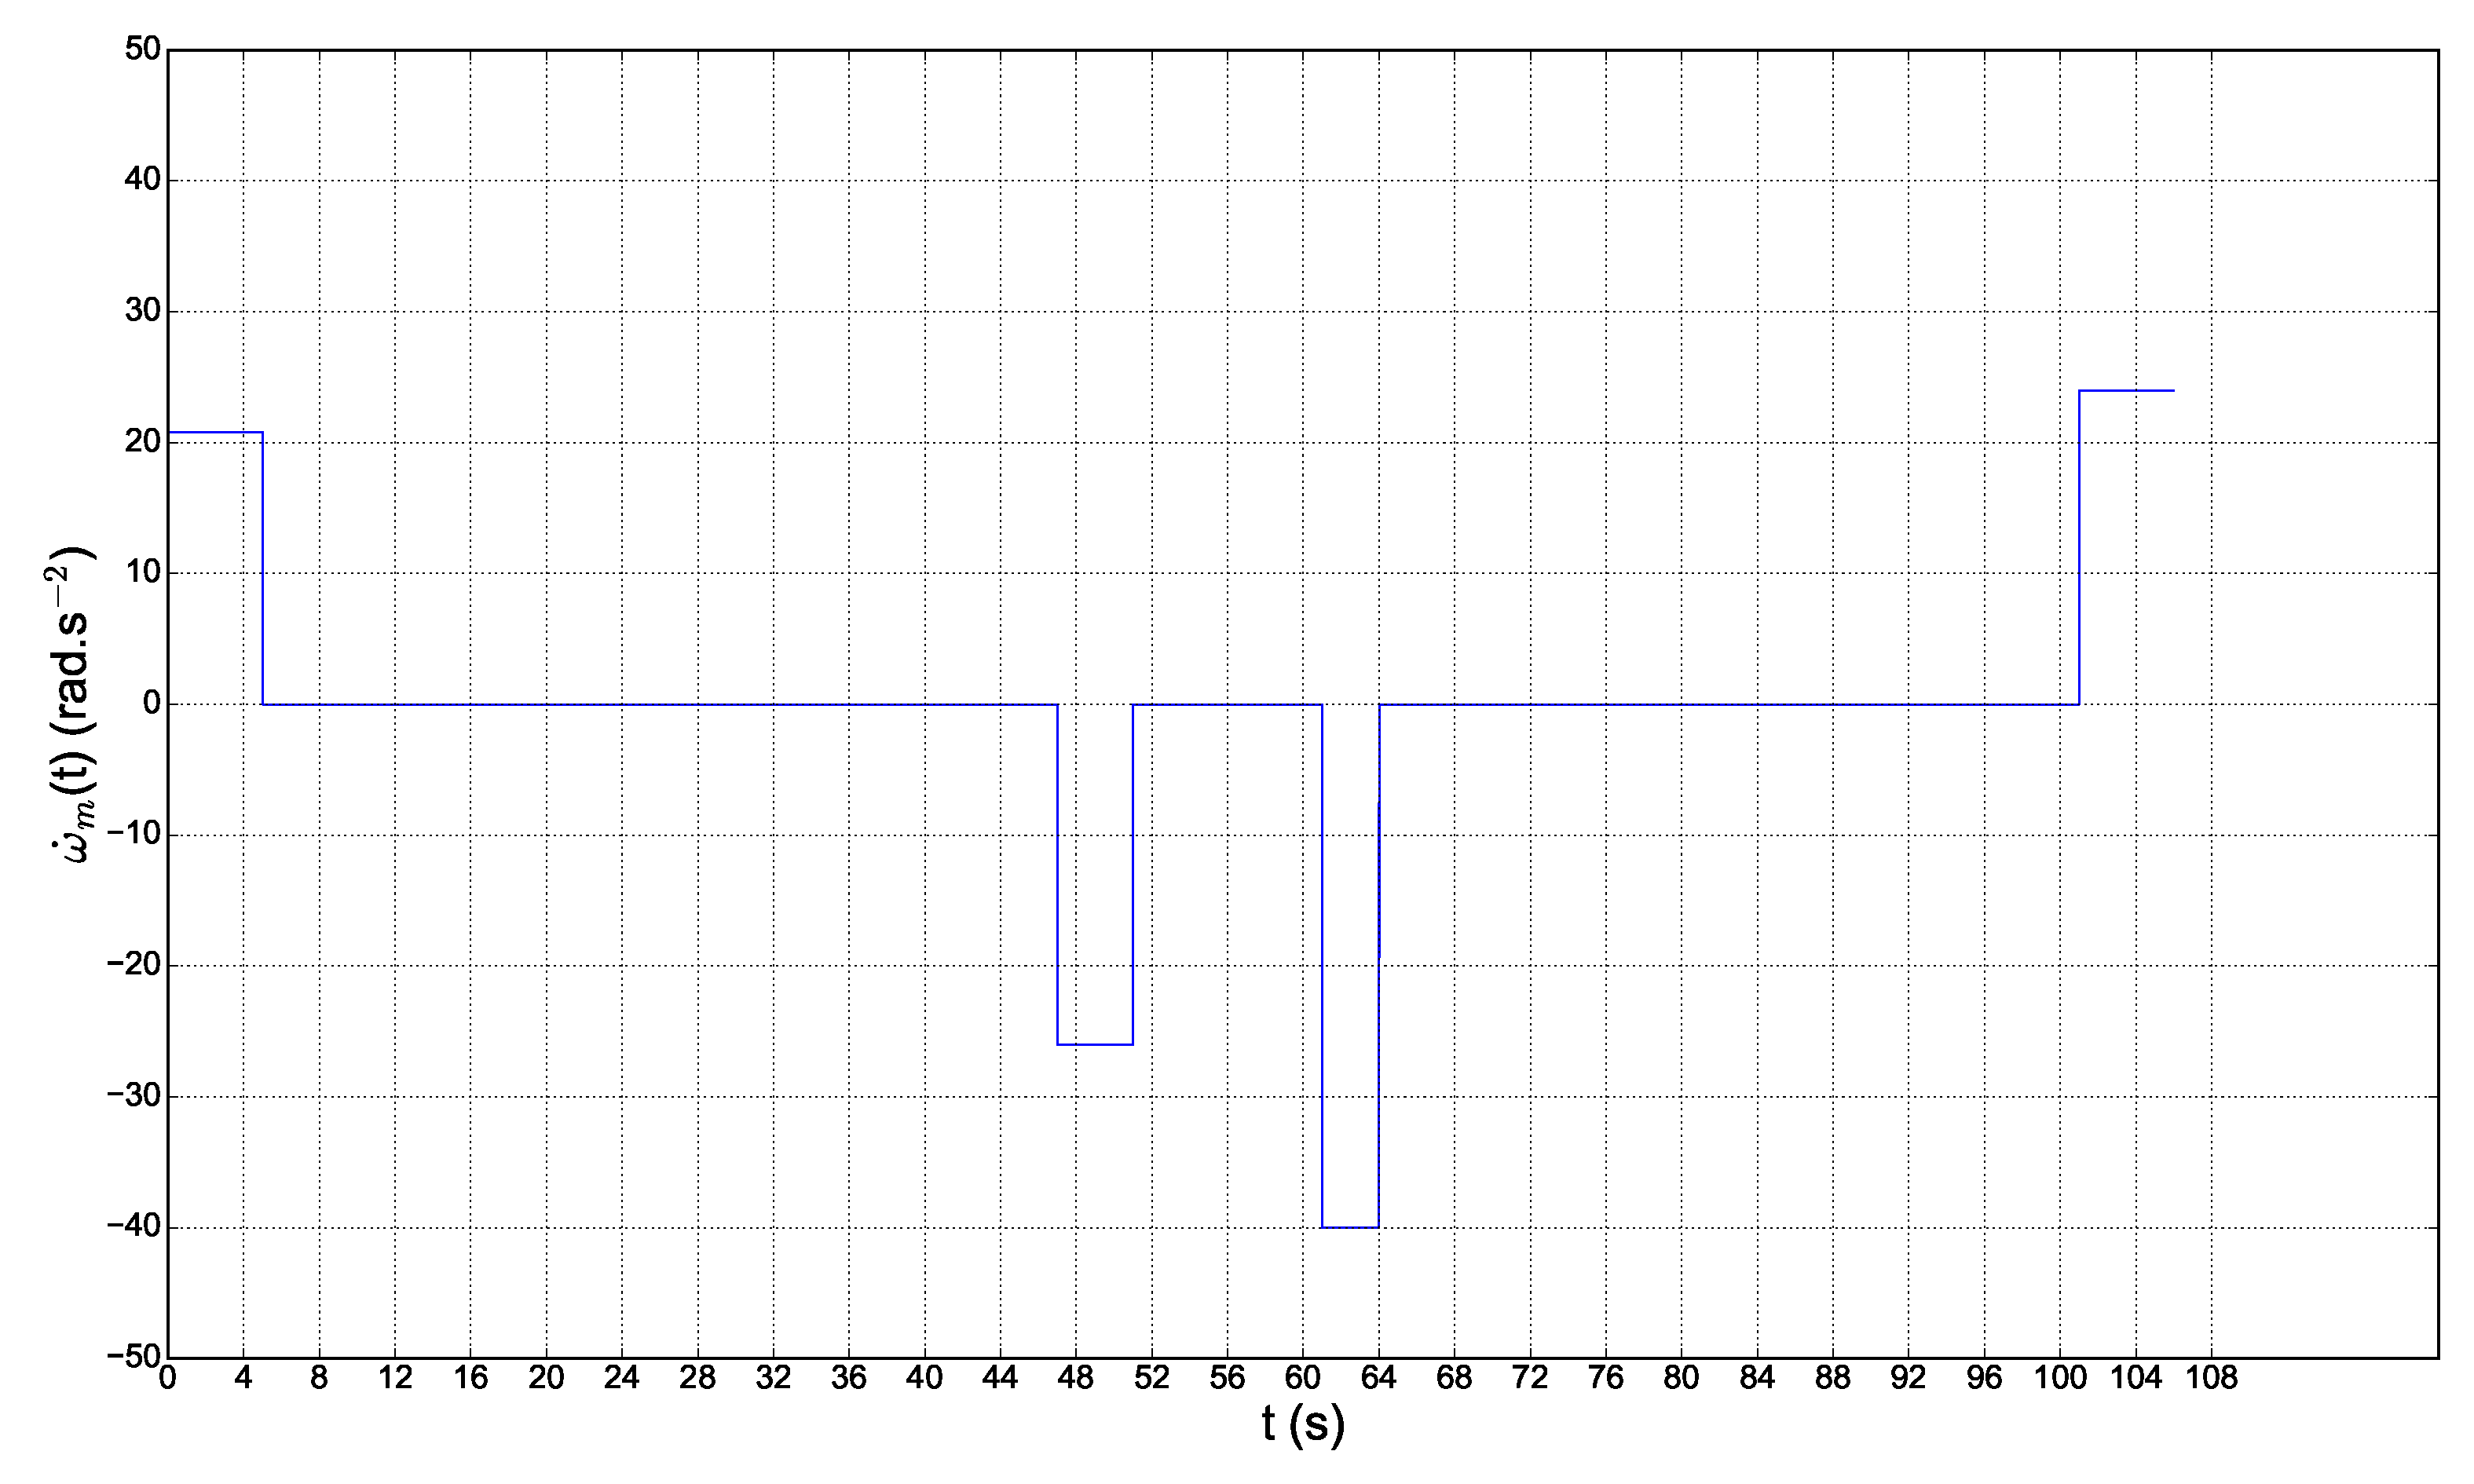
\includegraphics[width=0.9\linewidth]{img/accel_cor}
\end{center}

\reponse{12}{0}

$C_m(t)=J_{eq}.\frac{d\omega_m(t)}{dt}+\frac{\eta.M.g.p.k}{2.\pi}$

\begin{center}
 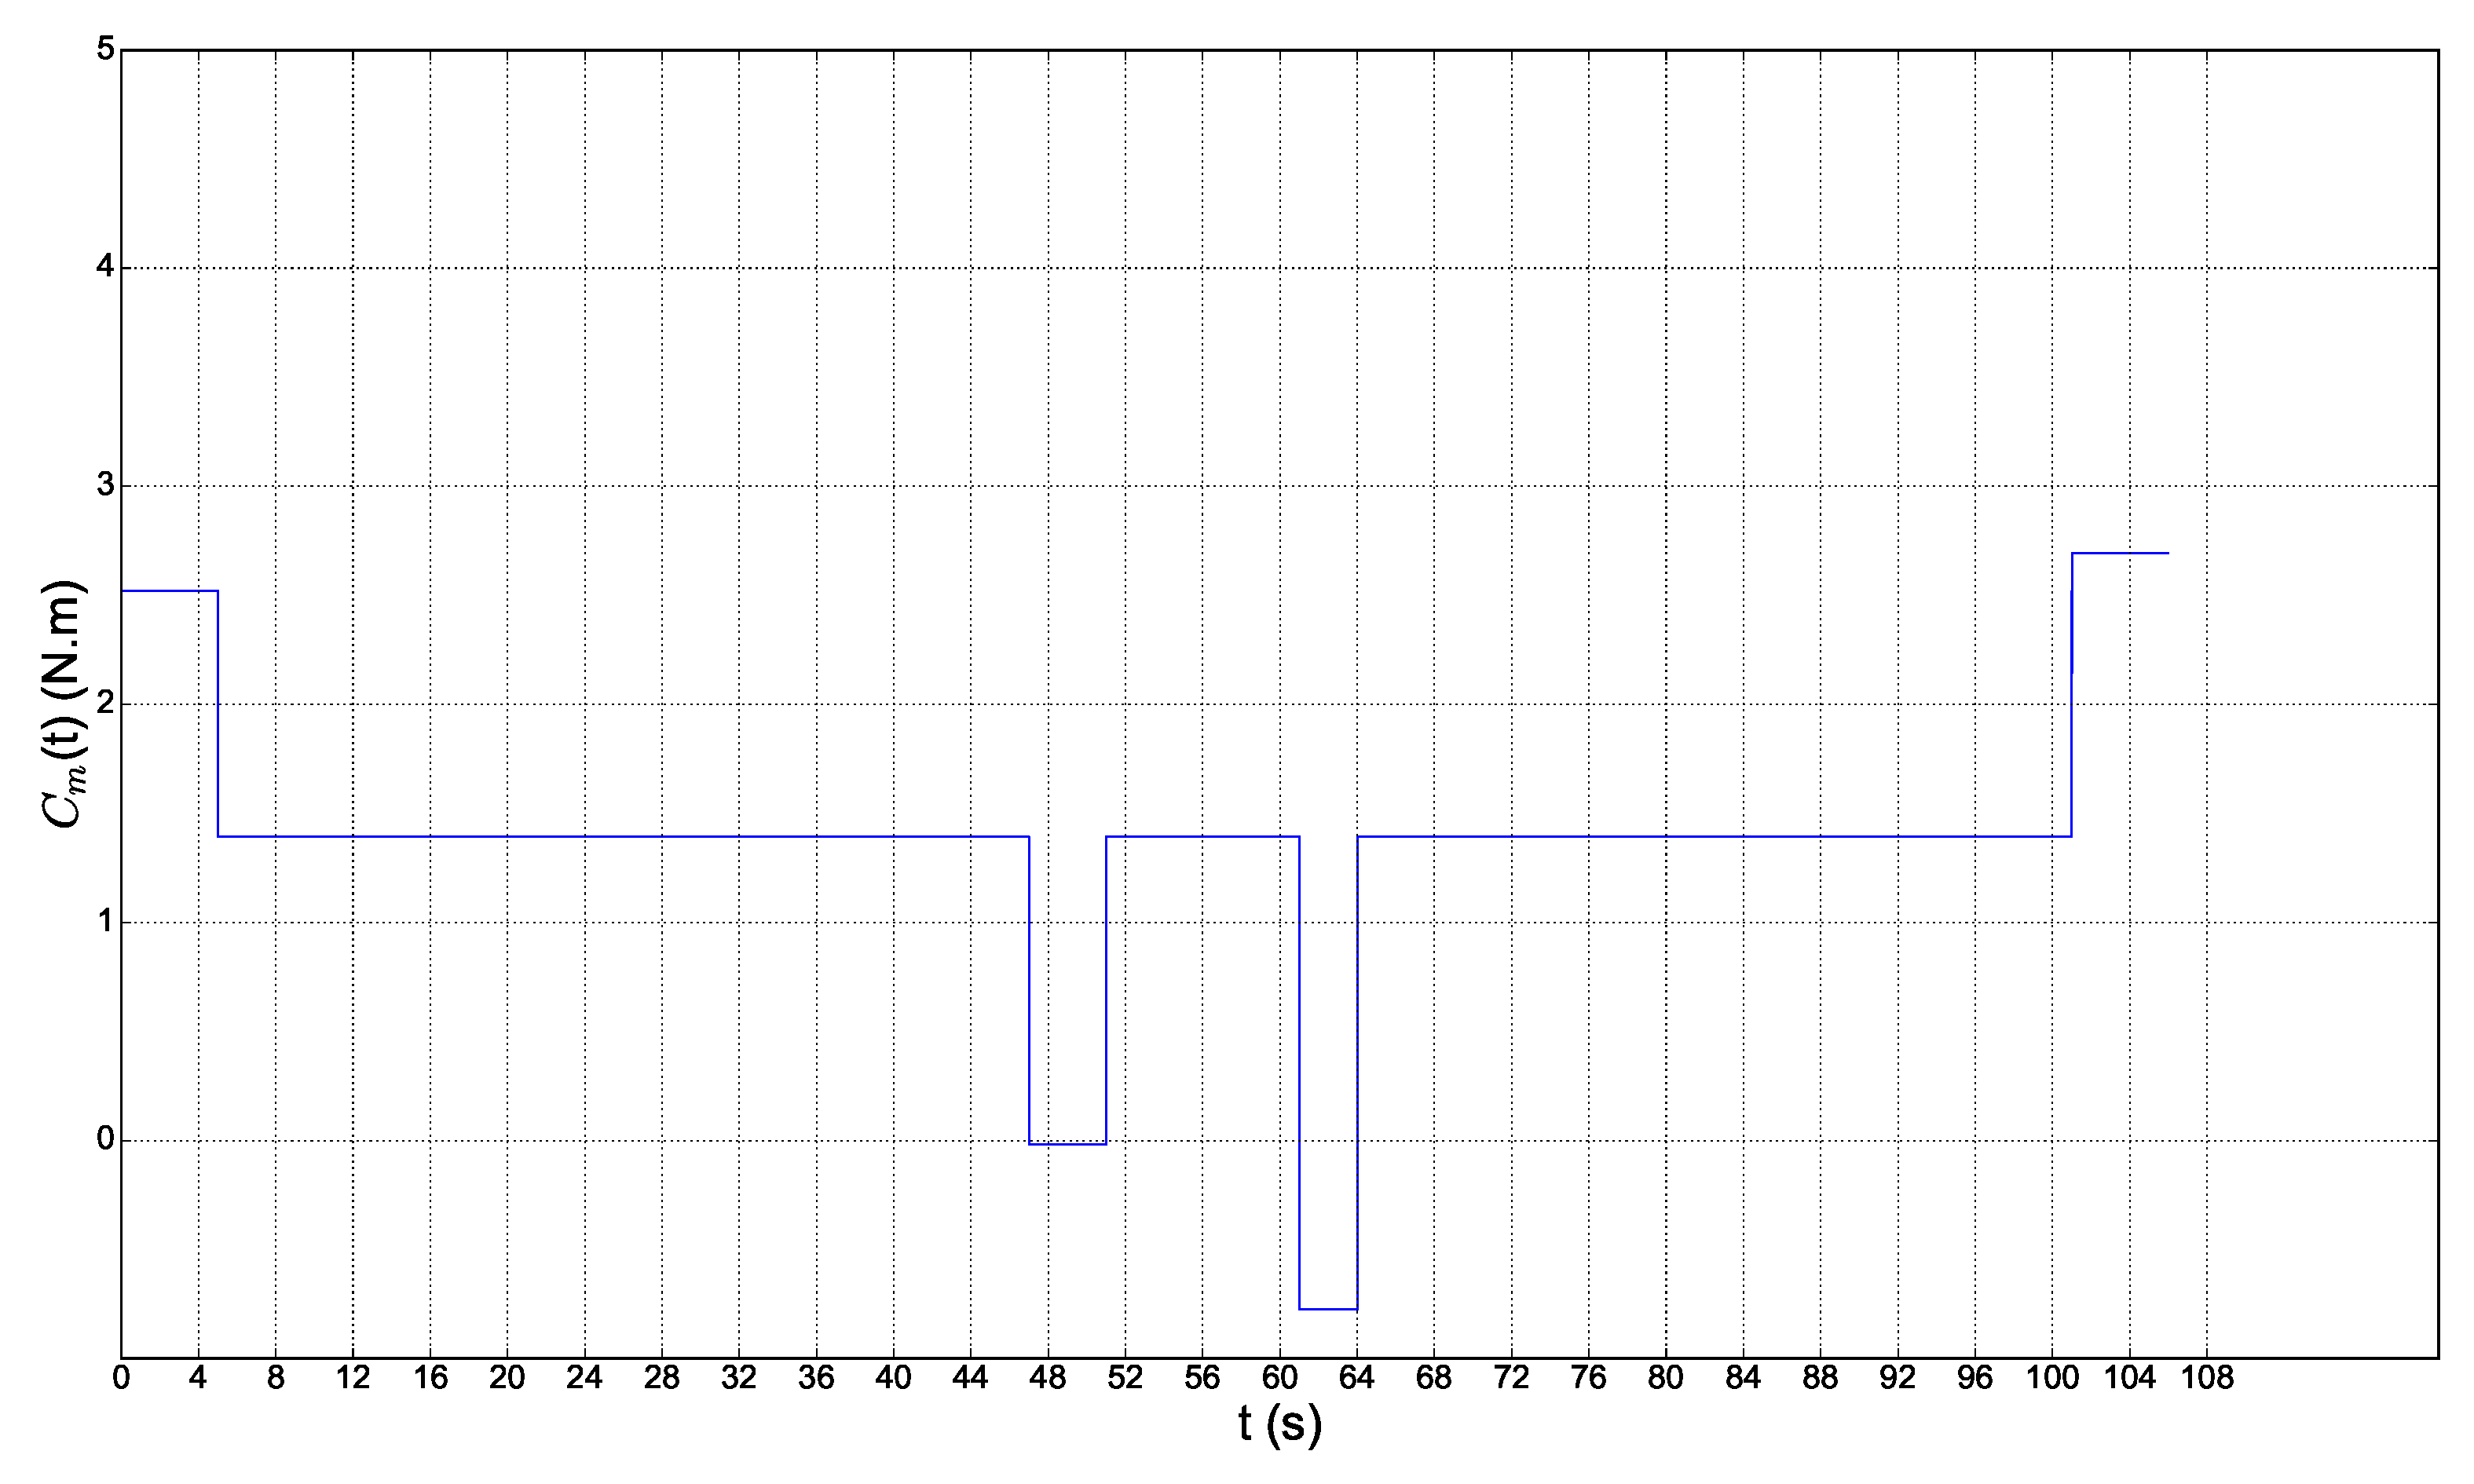
\includegraphics[width=0.9\linewidth]{img/couple_cor}
\end{center}

\reponse{13}{0}

La vitesse de rotation est inférieure à $1080tr.min^{-1}=113rad.s^{-1}$, le couple est inférieur à $6,46N.m$, le moteur correspond donc aux performances attendues.

\reponse{14}{0}

\begin{center}
 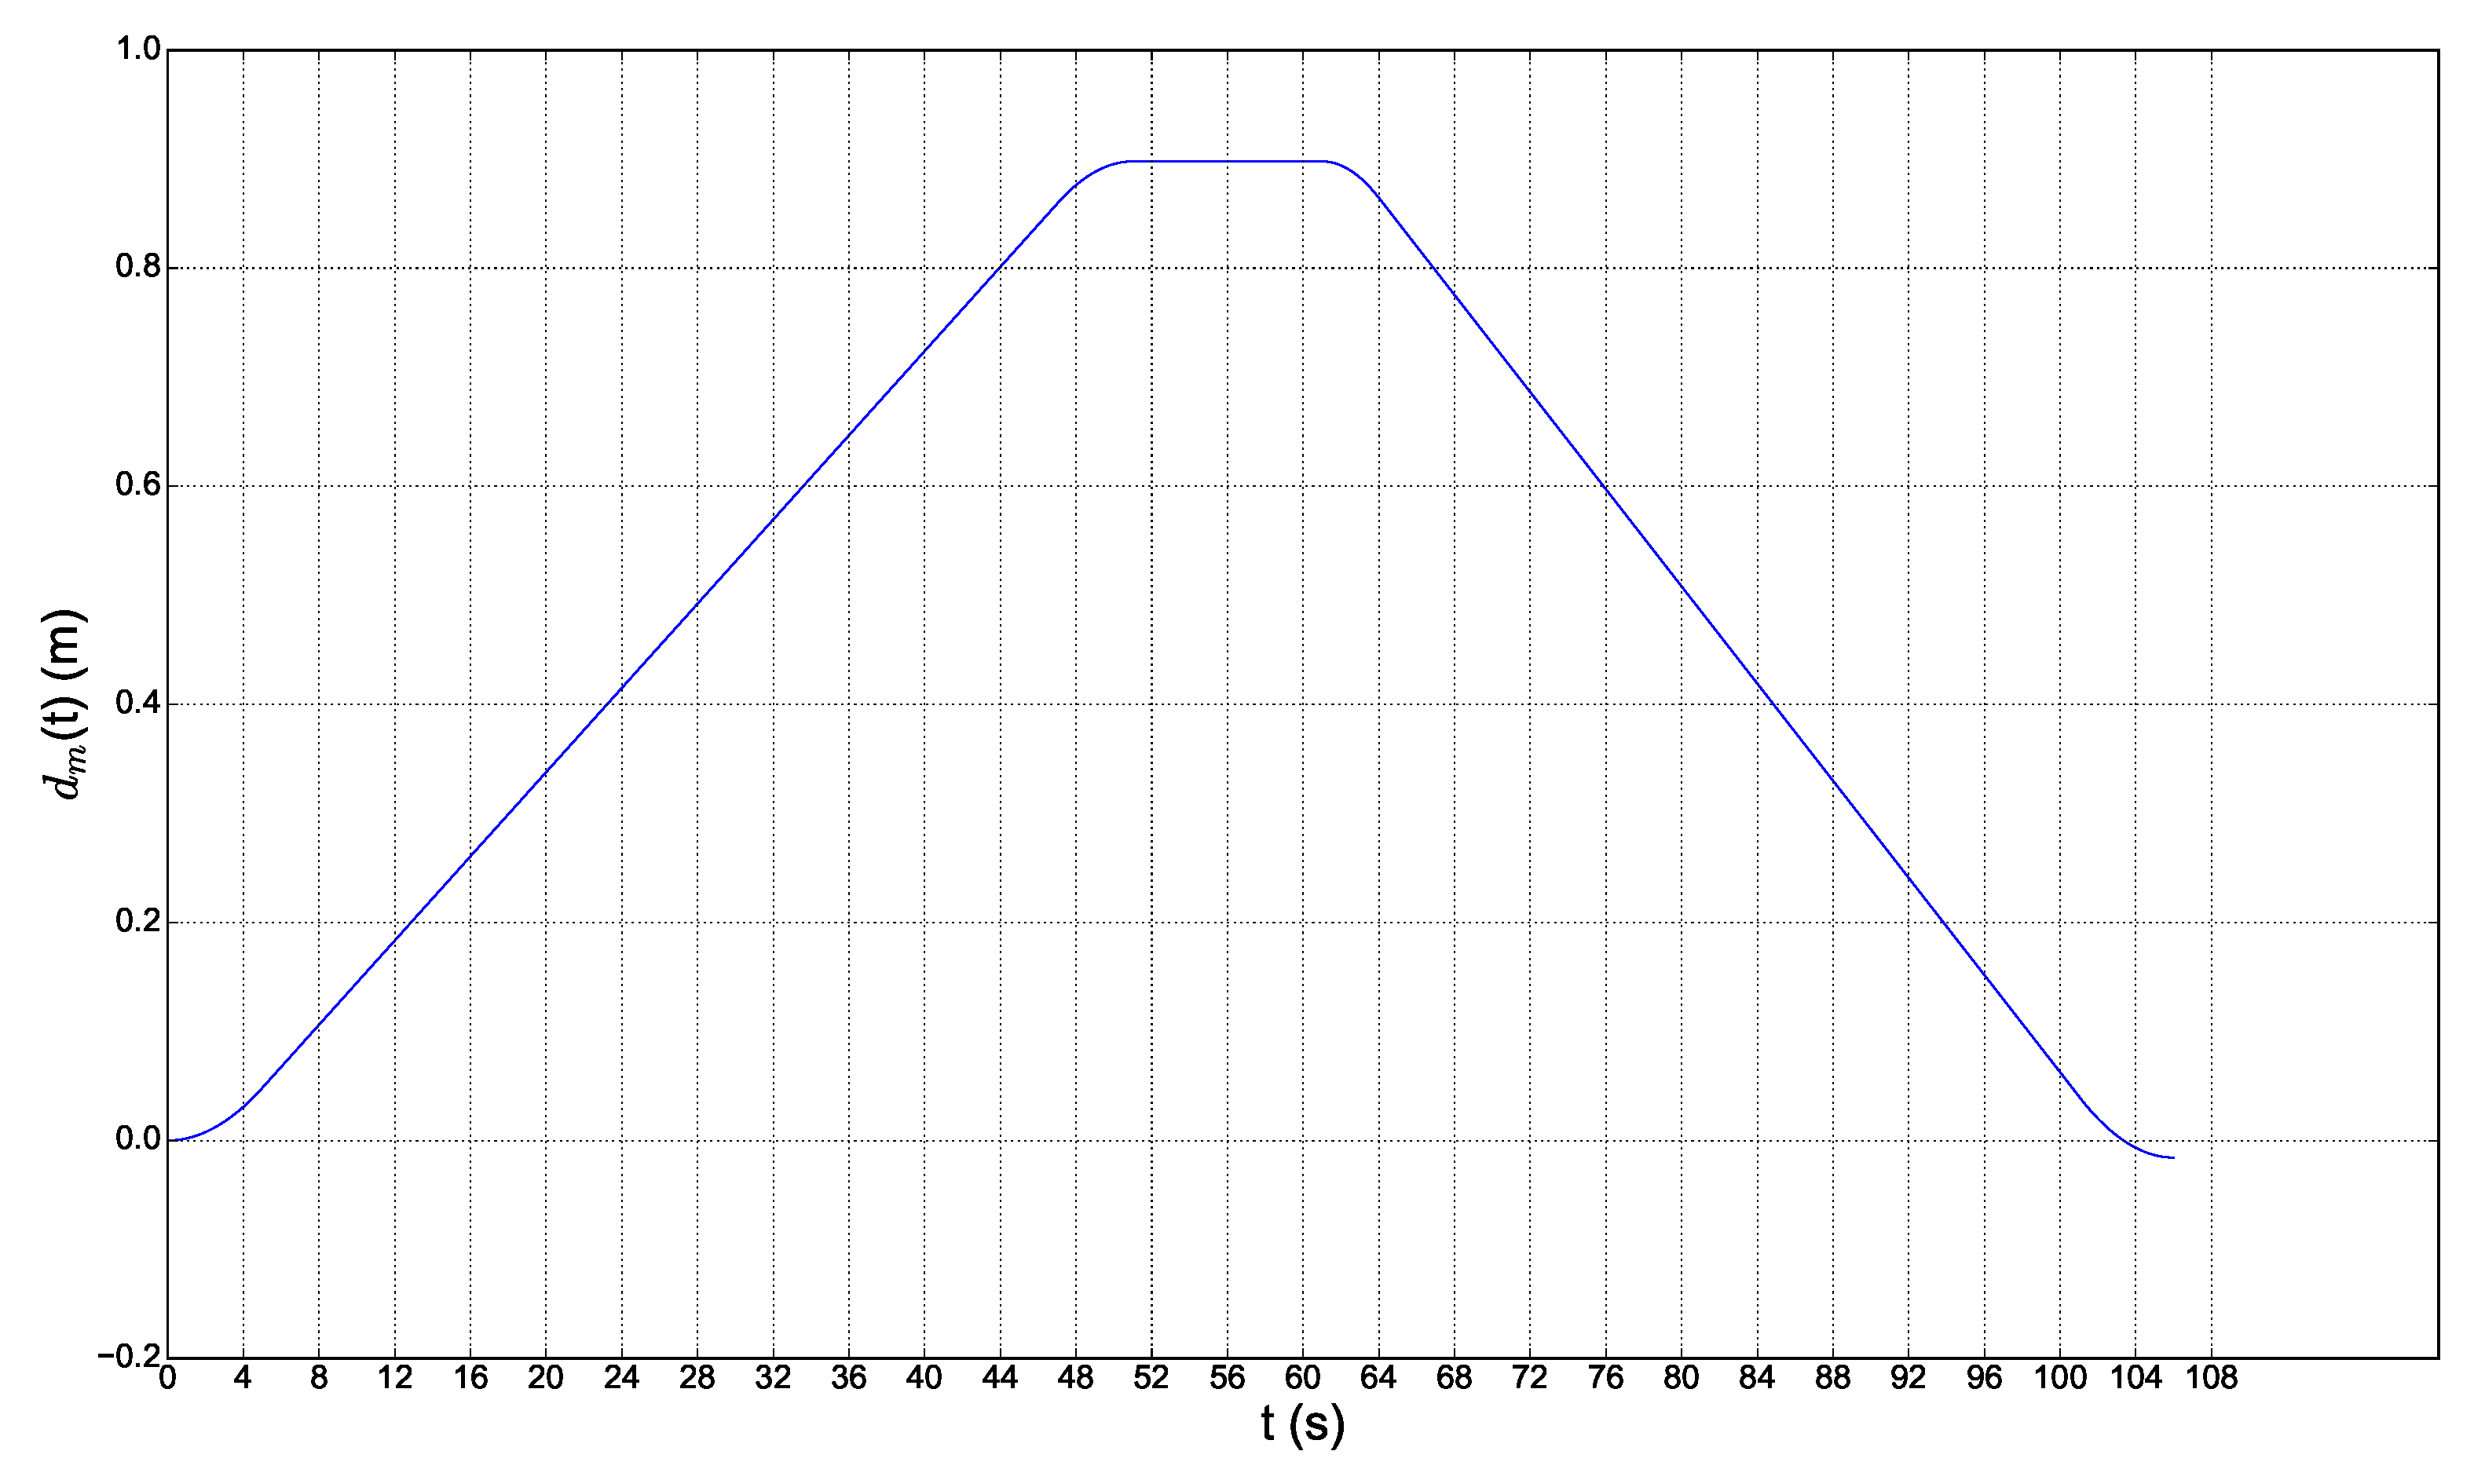
\includegraphics[width=0.9\linewidth]{img/deplacement_cor}
\end{center}

\reponse{15}{0}

Le déplacement de 0,9m correspond à celui du cahier des charges.

\reponse{16}{0}

$\left\{\begin{array}{l}
u(t)=R.i(t)+L.\frac{di(t)}{dt}+e(t) \\
e(t)=K_e.\omega_m(t) \\
C_m=K_c.i(t)
\end{array}\right.$

\reponse{17}{0}

$u(t)=\frac{R}{K_c}.C_m(t)+\frac{L}{K_c}.\frac{dC_m(t)}{dt}+K_e.\omega_m(t)$

\reponse{18}{0}

$u(t)=\frac{R}{K_c}.C_m(t)+K_e.\omega_m(t)$

\reponse{19}{0}

\begin{center}
 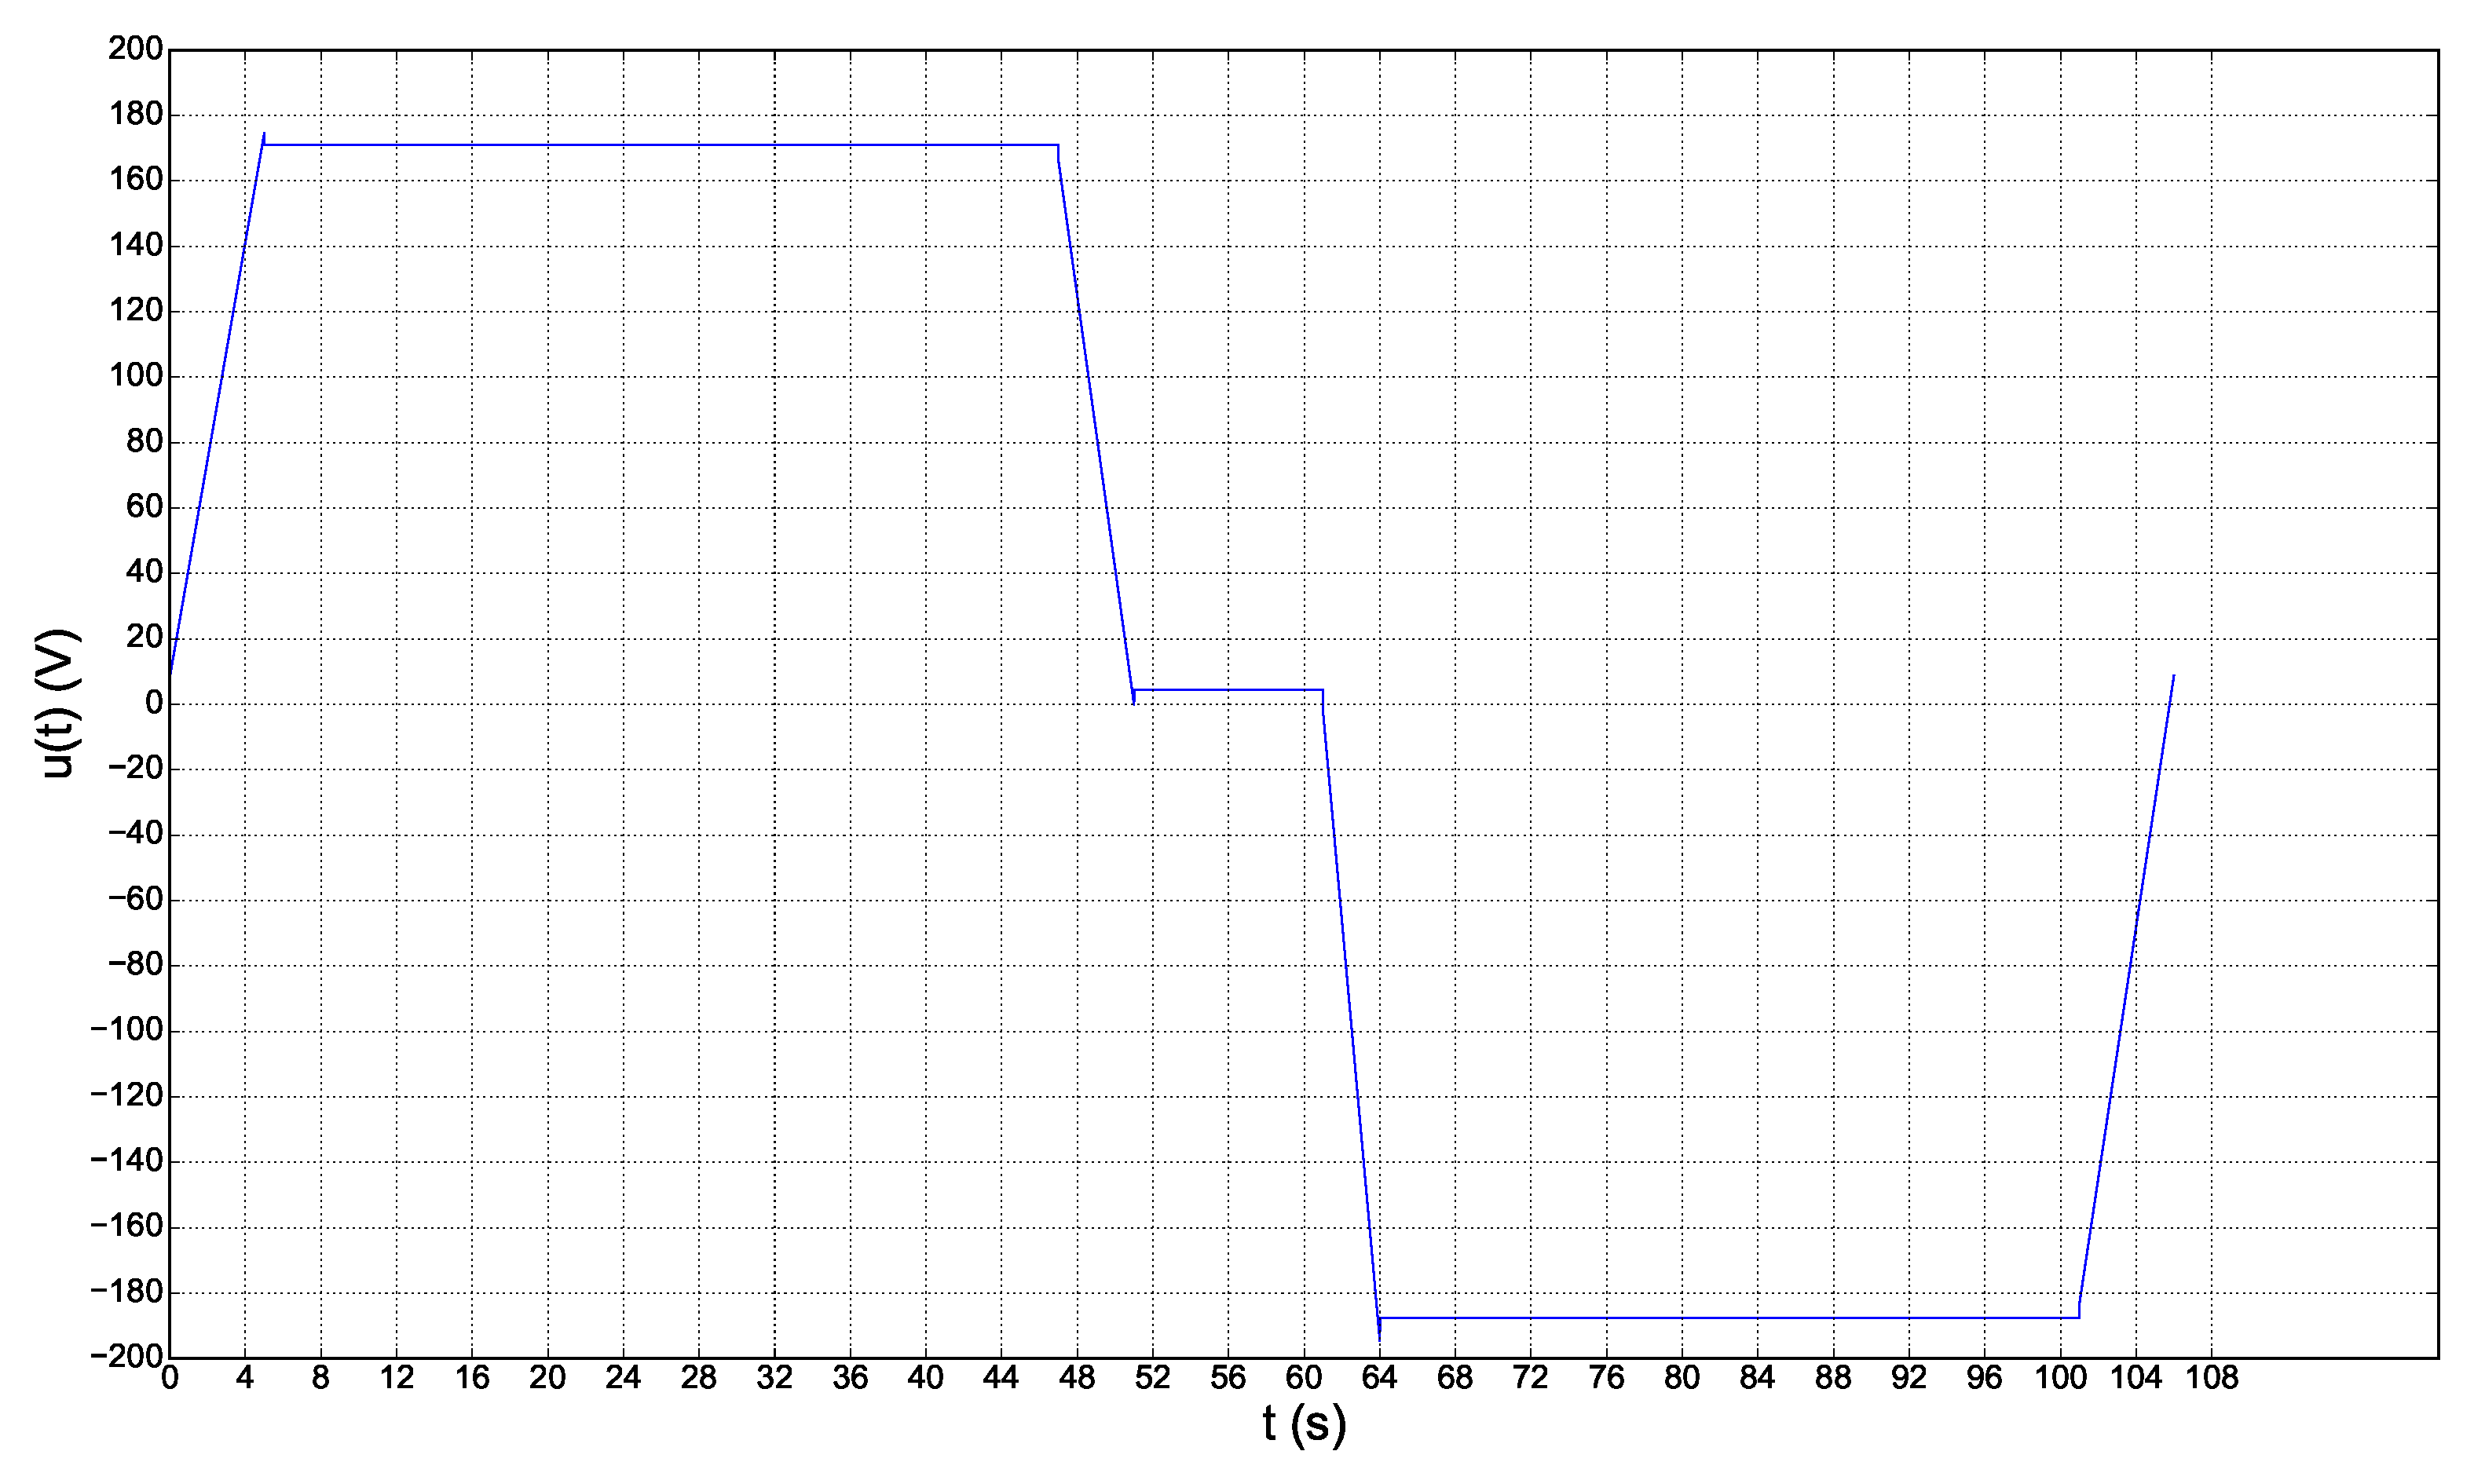
\includegraphics[width=0.9\linewidth]{img/tension_cor}
\end{center}

\reponse{20}{0}

Cette valeur est inférieure à $230V$, elle est donc compatible avec les caractéristiques nominales du moteur.

\reponse{21}{0}

Le couple ne variant pas de façon continue, la dérivée $\frac{dC_m(t)}{dt}$ serait infinie, ce qui ne permettrait pas de répondre aux question 18 et 19.

\reponse{22}{0}

Ce profil est théorique et ne peut 
\end{document}
